% Options for packages loaded elsewhere
\PassOptionsToPackage{unicode}{hyperref}
\PassOptionsToPackage{hyphens}{url}
\PassOptionsToPackage{dvipsnames,svgnames,x11names}{xcolor}
%
\documentclass[
  letterpaper,
  DIV=11,
  numbers=noendperiod]{scrreprt}

\usepackage{amsmath,amssymb}
\usepackage{iftex}
\ifPDFTeX
  \usepackage[T1]{fontenc}
  \usepackage[utf8]{inputenc}
  \usepackage{textcomp} % provide euro and other symbols
\else % if luatex or xetex
  \usepackage{unicode-math}
  \defaultfontfeatures{Scale=MatchLowercase}
  \defaultfontfeatures[\rmfamily]{Ligatures=TeX,Scale=1}
\fi
\usepackage{lmodern}
\ifPDFTeX\else  
    % xetex/luatex font selection
\fi
% Use upquote if available, for straight quotes in verbatim environments
\IfFileExists{upquote.sty}{\usepackage{upquote}}{}
\IfFileExists{microtype.sty}{% use microtype if available
  \usepackage[]{microtype}
  \UseMicrotypeSet[protrusion]{basicmath} % disable protrusion for tt fonts
}{}
\makeatletter
\@ifundefined{KOMAClassName}{% if non-KOMA class
  \IfFileExists{parskip.sty}{%
    \usepackage{parskip}
  }{% else
    \setlength{\parindent}{0pt}
    \setlength{\parskip}{6pt plus 2pt minus 1pt}}
}{% if KOMA class
  \KOMAoptions{parskip=half}}
\makeatother
\usepackage{xcolor}
\setlength{\emergencystretch}{3em} % prevent overfull lines
\setcounter{secnumdepth}{5}
% Make \paragraph and \subparagraph free-standing
\makeatletter
\ifx\paragraph\undefined\else
  \let\oldparagraph\paragraph
  \renewcommand{\paragraph}{
    \@ifstar
      \xxxParagraphStar
      \xxxParagraphNoStar
  }
  \newcommand{\xxxParagraphStar}[1]{\oldparagraph*{#1}\mbox{}}
  \newcommand{\xxxParagraphNoStar}[1]{\oldparagraph{#1}\mbox{}}
\fi
\ifx\subparagraph\undefined\else
  \let\oldsubparagraph\subparagraph
  \renewcommand{\subparagraph}{
    \@ifstar
      \xxxSubParagraphStar
      \xxxSubParagraphNoStar
  }
  \newcommand{\xxxSubParagraphStar}[1]{\oldsubparagraph*{#1}\mbox{}}
  \newcommand{\xxxSubParagraphNoStar}[1]{\oldsubparagraph{#1}\mbox{}}
\fi
\makeatother

\usepackage{color}
\usepackage{fancyvrb}
\newcommand{\VerbBar}{|}
\newcommand{\VERB}{\Verb[commandchars=\\\{\}]}
\DefineVerbatimEnvironment{Highlighting}{Verbatim}{commandchars=\\\{\}}
% Add ',fontsize=\small' for more characters per line
\usepackage{framed}
\definecolor{shadecolor}{RGB}{241,243,245}
\newenvironment{Shaded}{\begin{snugshade}}{\end{snugshade}}
\newcommand{\AlertTok}[1]{\textcolor[rgb]{0.68,0.00,0.00}{#1}}
\newcommand{\AnnotationTok}[1]{\textcolor[rgb]{0.37,0.37,0.37}{#1}}
\newcommand{\AttributeTok}[1]{\textcolor[rgb]{0.40,0.45,0.13}{#1}}
\newcommand{\BaseNTok}[1]{\textcolor[rgb]{0.68,0.00,0.00}{#1}}
\newcommand{\BuiltInTok}[1]{\textcolor[rgb]{0.00,0.23,0.31}{#1}}
\newcommand{\CharTok}[1]{\textcolor[rgb]{0.13,0.47,0.30}{#1}}
\newcommand{\CommentTok}[1]{\textcolor[rgb]{0.37,0.37,0.37}{#1}}
\newcommand{\CommentVarTok}[1]{\textcolor[rgb]{0.37,0.37,0.37}{\textit{#1}}}
\newcommand{\ConstantTok}[1]{\textcolor[rgb]{0.56,0.35,0.01}{#1}}
\newcommand{\ControlFlowTok}[1]{\textcolor[rgb]{0.00,0.23,0.31}{\textbf{#1}}}
\newcommand{\DataTypeTok}[1]{\textcolor[rgb]{0.68,0.00,0.00}{#1}}
\newcommand{\DecValTok}[1]{\textcolor[rgb]{0.68,0.00,0.00}{#1}}
\newcommand{\DocumentationTok}[1]{\textcolor[rgb]{0.37,0.37,0.37}{\textit{#1}}}
\newcommand{\ErrorTok}[1]{\textcolor[rgb]{0.68,0.00,0.00}{#1}}
\newcommand{\ExtensionTok}[1]{\textcolor[rgb]{0.00,0.23,0.31}{#1}}
\newcommand{\FloatTok}[1]{\textcolor[rgb]{0.68,0.00,0.00}{#1}}
\newcommand{\FunctionTok}[1]{\textcolor[rgb]{0.28,0.35,0.67}{#1}}
\newcommand{\ImportTok}[1]{\textcolor[rgb]{0.00,0.46,0.62}{#1}}
\newcommand{\InformationTok}[1]{\textcolor[rgb]{0.37,0.37,0.37}{#1}}
\newcommand{\KeywordTok}[1]{\textcolor[rgb]{0.00,0.23,0.31}{\textbf{#1}}}
\newcommand{\NormalTok}[1]{\textcolor[rgb]{0.00,0.23,0.31}{#1}}
\newcommand{\OperatorTok}[1]{\textcolor[rgb]{0.37,0.37,0.37}{#1}}
\newcommand{\OtherTok}[1]{\textcolor[rgb]{0.00,0.23,0.31}{#1}}
\newcommand{\PreprocessorTok}[1]{\textcolor[rgb]{0.68,0.00,0.00}{#1}}
\newcommand{\RegionMarkerTok}[1]{\textcolor[rgb]{0.00,0.23,0.31}{#1}}
\newcommand{\SpecialCharTok}[1]{\textcolor[rgb]{0.37,0.37,0.37}{#1}}
\newcommand{\SpecialStringTok}[1]{\textcolor[rgb]{0.13,0.47,0.30}{#1}}
\newcommand{\StringTok}[1]{\textcolor[rgb]{0.13,0.47,0.30}{#1}}
\newcommand{\VariableTok}[1]{\textcolor[rgb]{0.07,0.07,0.07}{#1}}
\newcommand{\VerbatimStringTok}[1]{\textcolor[rgb]{0.13,0.47,0.30}{#1}}
\newcommand{\WarningTok}[1]{\textcolor[rgb]{0.37,0.37,0.37}{\textit{#1}}}

\providecommand{\tightlist}{%
  \setlength{\itemsep}{0pt}\setlength{\parskip}{0pt}}\usepackage{longtable,booktabs,array}
\usepackage{calc} % for calculating minipage widths
% Correct order of tables after \paragraph or \subparagraph
\usepackage{etoolbox}
\makeatletter
\patchcmd\longtable{\par}{\if@noskipsec\mbox{}\fi\par}{}{}
\makeatother
% Allow footnotes in longtable head/foot
\IfFileExists{footnotehyper.sty}{\usepackage{footnotehyper}}{\usepackage{footnote}}
\makesavenoteenv{longtable}
\usepackage{graphicx}
\makeatletter
\def\maxwidth{\ifdim\Gin@nat@width>\linewidth\linewidth\else\Gin@nat@width\fi}
\def\maxheight{\ifdim\Gin@nat@height>\textheight\textheight\else\Gin@nat@height\fi}
\makeatother
% Scale images if necessary, so that they will not overflow the page
% margins by default, and it is still possible to overwrite the defaults
% using explicit options in \includegraphics[width, height, ...]{}
\setkeys{Gin}{width=\maxwidth,height=\maxheight,keepaspectratio}
% Set default figure placement to htbp
\makeatletter
\def\fps@figure{htbp}
\makeatother

\KOMAoption{captions}{tableheading}
\makeatletter
\@ifpackageloaded{tcolorbox}{}{\usepackage[skins,breakable]{tcolorbox}}
\@ifpackageloaded{fontawesome5}{}{\usepackage{fontawesome5}}
\definecolor{quarto-callout-color}{HTML}{909090}
\definecolor{quarto-callout-note-color}{HTML}{0758E5}
\definecolor{quarto-callout-important-color}{HTML}{CC1914}
\definecolor{quarto-callout-warning-color}{HTML}{EB9113}
\definecolor{quarto-callout-tip-color}{HTML}{00A047}
\definecolor{quarto-callout-caution-color}{HTML}{FC5300}
\definecolor{quarto-callout-color-frame}{HTML}{acacac}
\definecolor{quarto-callout-note-color-frame}{HTML}{4582ec}
\definecolor{quarto-callout-important-color-frame}{HTML}{d9534f}
\definecolor{quarto-callout-warning-color-frame}{HTML}{f0ad4e}
\definecolor{quarto-callout-tip-color-frame}{HTML}{02b875}
\definecolor{quarto-callout-caution-color-frame}{HTML}{fd7e14}
\makeatother
\makeatletter
\@ifpackageloaded{bookmark}{}{\usepackage{bookmark}}
\makeatother
\makeatletter
\@ifpackageloaded{caption}{}{\usepackage{caption}}
\AtBeginDocument{%
\ifdefined\contentsname
  \renewcommand*\contentsname{Table of contents}
\else
  \newcommand\contentsname{Table of contents}
\fi
\ifdefined\listfigurename
  \renewcommand*\listfigurename{List of Figures}
\else
  \newcommand\listfigurename{List of Figures}
\fi
\ifdefined\listtablename
  \renewcommand*\listtablename{List of Tables}
\else
  \newcommand\listtablename{List of Tables}
\fi
\ifdefined\figurename
  \renewcommand*\figurename{Figure}
\else
  \newcommand\figurename{Figure}
\fi
\ifdefined\tablename
  \renewcommand*\tablename{Table}
\else
  \newcommand\tablename{Table}
\fi
}
\@ifpackageloaded{float}{}{\usepackage{float}}
\floatstyle{ruled}
\@ifundefined{c@chapter}{\newfloat{codelisting}{h}{lop}}{\newfloat{codelisting}{h}{lop}[chapter]}
\floatname{codelisting}{Listing}
\newcommand*\listoflistings{\listof{codelisting}{List of Listings}}
\makeatother
\makeatletter
\makeatother
\makeatletter
\@ifpackageloaded{caption}{}{\usepackage{caption}}
\@ifpackageloaded{subcaption}{}{\usepackage{subcaption}}
\makeatother

\ifLuaTeX
  \usepackage{selnolig}  % disable illegal ligatures
\fi
\usepackage{bookmark}

\IfFileExists{xurl.sty}{\usepackage{xurl}}{} % add URL line breaks if available
\urlstyle{same} % disable monospaced font for URLs
\hypersetup{
  pdftitle={Estadística para Ciencias Sociales},
  pdfauthor={Julián Cruz},
  colorlinks=true,
  linkcolor={blue},
  filecolor={Maroon},
  citecolor={Blue},
  urlcolor={Blue},
  pdfcreator={LaTeX via pandoc}}


\title{Estadística para Ciencias Sociales}
\author{Julián Cruz}
\date{}

\begin{document}
\maketitle

\renewcommand*\contentsname{Table of contents}
{
\hypersetup{linkcolor=}
\setcounter{tocdepth}{2}
\tableofcontents
}

\bookmarksetup{startatroot}

\chapter*{Comencemos}\label{comencemos}
\addcontentsline{toc}{chapter}{Comencemos}

\markboth{Comencemos}{Comencemos}

\begin{Shaded}
\begin{Highlighting}[]
\CommentTok{\# justificar los textos vía css}
\CommentTok{\# Pruebas de hipótesis: analíticas paramétricas, analíticas no paramétricas, computacionales paramétricas, computacionales no paramétricas.}
\CommentTok{\# Poner todas las fórmulas en cajas}
\CommentTok{\# Variables cualitativas, cómo se ven en un gráfico, cuáles son sus elementos visuales, cómo se trabajan en modelamiento, datos cíclicos, datos textuales}
\CommentTok{\# Hacer capítulo de preparación de los datos.}
\DocumentationTok{\#\#\#\# Completar la fórmula de las estadíustias descriptivas}
\CommentTok{\# Actualizar los covers para que coincidan con los capítulos}
\end{Highlighting}
\end{Shaded}

El Laboratorio Interdisciplinar de Medición Social (LABMEDISOCIAL) se
complace en presentar estas notas de clase sobre estadística en ciencias
sociales.

La estadística, en su esencia, constituye un puente entre la observación
empírica y la construcción de conocimiento científico. En el ámbito de
las ciencias sociales, su aplicación trasciende el análisis de datos
para convertirse en una herramienta indispensable en la formulación de
teorías, la validación de hipótesis y la toma de decisiones
fundamentadas. Este libro se concibe como una contribución a ese
esfuerzo, ofreciendo una integración rigurosa de fundamentos teóricos y
aplicaciones prácticas, sustentada en la investigación social.

En investigación social, el uso adecuado de métodos estadísticos para
comprender la estructura y operatividad de un fenómeno determinado,
constituye una ventaja del investigador en un entorno competitio de alto
desempaño. Una gran variedad de procesos de planeación y evaluación de
actividades gubernamentales, administrativas, económicas y financieras,
se basan en resultados obtenidos mediante el análisis estadístico de los
fenómenos en ellos involucrados.

Además, dado el crecimiento exponencial de las fuentes de información y
el desarrollo acelerado de las herramientas tecnológicas, es apropiado
disponer de una sólida fundamentación conceptual y práctica que le
permita transformar y comprender grandes cantidades de información.

\section*{Material}\label{material}
\addcontentsline{toc}{section}{Material}

\markright{Material}

Los contenidos han sio generados utilizando modelos de generaci´no de
texto y consultando algunos materiales que se comparten a continuación.
Es importante prever que \textbf{algunos de estos vínculos pueden
caducar con el tiempo}, por lo cual no es raro que se pierda el acceso a
los materiales.

\href{https://openintro.org/book/os/}{OpenIntro Statistics}

\href{http://www.bnm.me.gov.ar/giga1/documentos/EL001858.pdf}{Estadística
para todos - Diana Kelmansky}

\href{https://ayushthey.medium.com/discourse-of-objectivity-2eb2541f7177}{Discourse
of Objectivity}

\href{https://www.stat.berkeley.edu/~aldous/157/Papers/shmueli.pdf}{To
explain or to predict}

\href{https://dialnet.unirioja.es/descarga/articulo/4942056.pdf}{Escalas
de medición - Jorge Coronado Padilla}

\href{https://scielo.conicyt.cl/pdf/ijmorphol/v35n1/art37.pdf}{Técnicas
de Muestreo sobre una Población a Estudio - Tamara Otzen, Carlos
Manterola}

\href{https://openintro.org/go/?id=os4_for_screen_readers&referrer=/book/os/index.php}{OpenIntro
Statistics - David Diez}

\href{https://openaccess.uoc.edu/bitstream/10609/148455/1/AnalisisBivariante.pdf}{Análisis
bivariante - Jordi Mas Elias}

\href{https://www.istat.it/wp-content/uploads/2014/06/Handbook-on-Constructing-Composite-Indicators.pdf}{Handbook
on Constructing Composite Indicators: Methodology and User Guide}

\href{https://core.ac.uk/download/pdf/47265078.pdf}{Diseño y validación
de instrumentos de medición}

\href{http://cda.psych.uiuc.edu/statistical_learning_course/Jolliffe\%20I.\%20Principal\%20Component\%20Analysis\%20(2ed.,\%20Springer,\%202002)(518s)_MVsa_.pdf}{Principal
Component Analysis}

\section*{Recopilación}\label{recopilaciuxf3n}
\addcontentsline{toc}{section}{Recopilación}

\markright{Recopilación}

La tarea de recopilar y organizar la información ha sido llevada a cabo
por Julián Cruz.

Científico de datos, profesional en estadística y magíster en ciencias,
con más de 15 años de experiencia demostrada en analítica y ciencia de
datos. Su perfil contempla desde liderazgo de programas de capacitación
y gestión del cambio, hasta ejecución proyectos de base tecnológica. A
través de esta experiencia ha desarrollado diferentes competencias, como
la orientación al valor en toma de decisiones, la conformación y
desarrollo de equipos de alto desempeño y la negociación integradora.

\part{Estadística descriptiva}

En esta primera sección se examina la estadística descriptiva. El
contenido ha sido seleccionado cuidadosamente con el fin de agregar
valor a los análisis cuantitativos que se proponen al interior de las
investigaciones en ciencias sociales.

\section*{Introducción}\label{introducciuxf3n}
\addcontentsline{toc}{section}{Introducción}

\markright{Introducción}

Este primer tema introduce a los estudiantes en los conceptos básicos de
la estadística, comenzando por una definición de estadística y su
relevancia en el análisis de datos. Se exploran los \textbf{tipos de
variables}, que incluyen \textbf{variables cualitativas} (nominales y
ordinales) y \textbf{cuantitativas} (discretas y continuas). A
continuación, se aborda la \textbf{tipología de preguntas} en encuestas,
diferenciando entre preguntas abiertas, cerradas y escalas, y cómo estas
se relacionan con la medición de las variables. También se presentan los
\textbf{tipos de encuestas}, clasificadas según el método de recolección
(presencial, telefónica, online, etc.), su estructura (estructuradas,
semi-estructuradas, no estructuradas) y los contextos en los que se
aplican, lo cual es fundamental para la adecuada recolección de datos en
cualquier estudio estadístico.

\section*{Muestreo}\label{muestreo}
\addcontentsline{toc}{section}{Muestreo}

\markright{Muestreo}

En este tema se abordan los fundamentos del \textbf{muestreo}, que es el
proceso de seleccionar una parte representativa de una población para
inferir conclusiones sobre el total. Se explican dos grandes tipos de
muestreo: \textbf{probabilístico} y \textbf{no probabilístico}. En el
muestreo probabilístico, cada elemento de la población tiene una
probabilidad conocida y no nula de ser seleccionado, y se estudian
técnicas como el \textbf{muestreo aleatorio simple}, el \textbf{muestreo
multietápico}, el \textbf{muestreo estratificado} y el \textbf{muestreo
por conglomerados}. En el muestreo no probabilístico, la selección no se
basa en probabilidades, sino en criterios subjetivos o conveniencia,
como el \textbf{muestreo por conveniencia}, \textbf{muestreo por cuotas}
o \textbf{bola de nieve}. Este tema profundiza en las ventajas y
limitaciones de cada enfoque, subrayando la importancia de la
representatividad de la muestra y cómo esto afecta los resultados y su
generalización.

\section*{Estadística descriptiva para una
variable}\label{estaduxedstica-descriptiva-para-una-variable}
\addcontentsline{toc}{section}{Estadística descriptiva para una
variable}

\markright{Estadística descriptiva para una variable}

La \textbf{estadística descriptiva para una variable} se centra en la
síntesis y descripción de los datos mediante medidas numéricas y
representaciones gráficas. Se examinan las \textbf{medidas de tendencia
central} como la media, la mediana y la moda, que resumen el
comportamiento típico de la variable. También se analizan las
\textbf{medidas de dispersión} como el rango, la varianza y la
desviación estándar, que describen la variabilidad en los datos. El tema
incluye el uso de \textbf{gráficos} como histogramas, gráficos de barras
y diagramas de caja para visualizar la distribución de los datos. Estas
herramientas permiten una comprensión clara de cómo los datos están
distribuidos y proporcionan una base sólida para la inferencia
estadística.

\section*{Estadística descriptiva para dos o más
variables}\label{estaduxedstica-descriptiva-para-dos-o-muxe1s-variables}
\addcontentsline{toc}{section}{Estadística descriptiva para dos o más
variables}

\markright{Estadística descriptiva para dos o más variables}

Este tema amplía el análisis de la estadística descriptiva a dos o más
variables, abordando técnicas para analizar relaciones y asociaciones
entre ellas. Se introducen las \textbf{tablas de contingencia} para
estudiar la relación entre dos variables cualitativas, así como las
\textbf{medidas de asociación} como el \textbf{coeficiente de
correlación de Pearson} y \textbf{Spearman} para variables
cuantitativas. También se discuten las \textbf{gráficas de dispersión}
para visualizar relaciones entre dos variables cuantitativas y cómo se
puede ajustar una \textbf{recta de regresión} para predecir una variable
en función de otra. Además, se examinan los \textbf{coeficientes de
correlación parcial} y \textbf{análisis multivariado} para explorar cómo
varias variables se relacionan simultáneamente, lo que permite una
comprensión más profunda de las interacciones dentro de los datos.

\chapter{Preliminares}\label{preliminares}

La estadística, en su concepción moderna, es el resultado de un extenso
desarrollo histórico y epistemológico que refleja la evolución del
pensamiento humano en su búsqueda de patrones y significados en la
incertidumbre. Sus raíces se remontan a la antigüedad, cuando
civilizaciones como las babilónicas y egipcias utilizaban conteos y
registros para la administración y predicción. Sin embargo, fue en el
Renacimiento, con la formalización del pensamiento probabilístico por
figuras como Gerolamo Cardano y Pierre de Fermat, cuando emergieron las
bases matemáticas que darían forma a su carácter científico.

La epistemología de la estadística comenzó a consolidarse en el siglo
XVIII, con las contribuciones de pensadores como Thomas Bayes, quien
introdujo un enfoque probabilístico basado en la actualización del
conocimiento, y Carl Friedrich Gauss, cuya teoría de errores cimentó el
papel de la estadística en la inferencia científica. A medida que el
método científico se institucionalizaba, la estadística se convirtió en
un vehículo para traducir fenómenos observables en explicaciones
cuantitativas, adoptando principios de objetividad, reproducibilidad y
rigor.

El siglo XX marcó una transformación paradigmática, impulsada por
avances en la teoría de conjuntos, el cálculo y la computación. La
estadística inferencial y la probabilidad frecuentista, promovidas por
Ronald A. Fisher, Jerzy Neyman y Egon Pearson, coexistieron con enfoques
bayesianos, destacando debates epistemológicos sobre la naturaleza del
azar y la inferencia. Esta diversidad metodológica enriqueció su
aplicabilidad, desde el diseño de experimentos hasta el análisis de
sistemas complejos en las ciencias sociales.

Hoy, la estadística es no solo un instrumento técnico, sino también un
lenguaje epistemológico que da forma a cómo entendemos la realidad. Su
desarrollo histórico subraya la tensión entre el dato y la
interpretación, entre el caos del mundo empírico y la búsqueda de orden
intelectual.

\section{La verdad y la objetividad}\label{la-verdad-y-la-objetividad}

La necesidad de procesar información es inherente al ser humano, un
reflejo de su insaciable curiosidad por comprender el mundo que lo
rodea. En un universo complejo e incierto, la información se presenta
como un recurso esencial para la supervivencia, la toma de decisiones y
la construcción de conocimiento. Sin procesarla, los datos brutos
carecen de significado; es mediante el análisis y la síntesis que
transformamos fragmentos dispersos en narrativas coherentes que guían
nuestra acción. Esta capacidad no solo nos define como especie, sino que
también alimenta nuestra aspiración más profunda: la búsqueda de la
verdad.

\subsection{¿Existe la verdad?}\label{existe-la-verdad}

La existencia de la verdad es una cuestión filosófica que ha desafiado a
pensadores desde tiempos antiguos. Para Platón, la verdad era una forma
ideal, un conocimiento absoluto al que solo se accedía mediante la
razón. En contraste, las tradiciones empiristas, como las de Aristóteles
o Locke, vincularon la verdad con la experiencia y la observación. Sin
embargo, estas concepciones comparten una premisa: que la verdad es algo
objetivo, independiente del observador.

En un sentido práctico, la verdad parece manifestarse en dos planos:
como correspondencia con la realidad y como coherencia lógica dentro de
un sistema de pensamiento. La primera implica que una afirmación es
verdadera si refleja fielmente un hecho, mientras que la segunda sugiere
que la verdad puede ser relativa a los marcos epistemológicos que la
sustentan. Esto lleva a una paradoja: aunque aspiramos a la objetividad,
nuestra percepción de la verdad está inevitablemente condicionada por
nuestra cultura, lenguaje y experiencia.

\section{Verdad y objetividad en la
modernidad}\label{verdad-y-objetividad-en-la-modernidad}

La modernidad abrazó un enfoque racionalista y científico de la verdad,
fundado en la fe en el progreso y en la capacidad humana de descubrir
leyes universales que rigen la naturaleza y la sociedad. Este paradigma,
influido por el empirismo y el método científico, promovió una visión de
la verdad como algo accesible a través del rigor metodológico y la
acumulación de evidencias. La Revolución Científica y la Ilustración,
con pensadores como Descartes, Kant y Newton, consolidaron esta noción,
priorizando la objetividad y la replicabilidad como criterios de
validez.

Sin embargo, esta confianza en la verdad objetiva también trajo
tensiones. Por un lado, el poder del conocimiento científico revolucionó
la tecnología, la medicina y la economía. Por otro, redujo la
complejidad humana y social a ecuaciones y categorías simplificadas,
marginando otras formas de saber, como las éticas, estéticas y
espirituales. La modernidad trató la verdad como una meta absoluta, pero
al hacerlo, a menudo ignoró las dimensiones subjetivas y plurales de la
experiencia humana.

La objetividad en la modernidad se concibe como un ideal epistemológico
central, que busca eliminar la influencia de valores, emociones o
prejuicios individuales en la producción de conocimiento. Este concepto
está profundamente enraizado en el contexto histórico, filosófico y
científico de la modernidad, un período caracterizado por la confianza
en la razón, el método científico y el progreso.

\subsection{El surgimiento de la objetividad
moderna}\label{el-surgimiento-de-la-objetividad-moderna}

La modernidad, influenciada por la Ilustración y la Revolución
Científica, estableció la objetividad como el estándar para alcanzar
verdades universales. Filósofos como Descartes promovieron una visión
racionalista en la que el pensamiento lógico y metódico podía superar
las limitaciones de la percepción subjetiva. La objetividad se convirtió
en un mecanismo para garantizar que el conocimiento no estuviera
contaminado por creencias personales, ideologías o tradiciones.

En este contexto, la ciencia se posicionó como el paradigma del
conocimiento objetivo. Galileo, Newton y otros pioneros de la ciencia
moderna formularon leyes universales que prometían describir la
naturaleza de manera imparcial. El método científico, con su énfasis en
la observación sistemática, la experimentación controlada y la
replicabilidad, se estableció como el camino hacia un conocimiento
fiable y verificable.

\subsection{Características de la objetividad en la
modernidad}\label{caracteruxedsticas-de-la-objetividad-en-la-modernidad}

\begin{enumerate}
\def\labelenumi{\arabic{enumi}.}
\item
  \textbf{Universalidad}: La objetividad buscaba verdades aplicables a
  todos los contextos, independientemente de las diferencias culturales,
  históricas o individuales. Por ejemplo, las leyes de la física se
  consideraron válidas tanto en Europa como en otras partes del mundo.
\item
  \textbf{Neutralidad}: La modernidad aspiraba a un conocimiento libre
  de intereses particulares, de manera que la investigación científica
  pudiera ser una empresa independiente de valores políticos, éticos o
  sociales.
\item
  \textbf{Rigor metódico}: La objetividad requería procedimientos
  estandarizados que redujeran al mínimo la influencia de sesgos
  personales. Esto incluía el uso de instrumentos de medición, controles
  experimentales y protocolos reproducibles.
\item
  \textbf{Despersonalización}: En aras de la objetividad, se promovió
  una separación entre el investigador y el objeto de estudio. El
  científico debía actuar como un observador distante, dejando a un lado
  emociones, creencias y deseos personales.
\end{enumerate}

\subsection{Críticas y tensiones}\label{cruxedticas-y-tensiones}

Aunque la objetividad en la modernidad permitió avances extraordinarios
en ciencia y tecnología, también generó críticas y tensiones. Una de las
principales críticas es que la objetividad moderna a menudo enmascara
los contextos sociales, políticos y culturales que inevitablemente
influyen en la producción de conocimiento. Por ejemplo, Donna Haraway
argumenta que todo conocimiento es situado, es decir, que está
condicionado por la perspectiva y el contexto del observador, incluso en
disciplinas científicas.

Asimismo, la idea de neutralidad ha sido cuestionada. La investigación
científica no está aislada de los intereses económicos y políticos: qué
se investiga, cómo se financia y cómo se aplica el conocimiento son
decisiones influenciadas por valores y estructuras de poder. En este
sentido, la objetividad moderna ha sido vista como una aspiración más
que como una realidad alcanzable.

La objetividad en la modernidad representó un ideal revolucionario que
buscaba superar la subjetividad individual y alcanzar verdades
universales mediante el rigor metodológico y la neutralidad. Aunque
permitió el desarrollo de un conocimiento confiable y replicable, sus
limitaciones y tensiones muestran que incluso los estándares más altos
de objetividad no están exentos de condicionamientos humanos. Este
reconocimiento no invalida su valor, sino que nos invita a reflexionar
críticamente sobre cómo construimos conocimiento en contextos históricos
y sociales específicos.

\section{Verdad y objetividad en la
postmodernidad}\label{verdad-y-objetividad-en-la-postmodernidad}

La postmodernidad desafió la narrrativa hegemónica de verdad universal,
cuestionando la existencia misma de una verdad universal. En este
contexto, pensadores como Michel Foucault, Jean-François Lyotard y
Jacques Derrida argumentaron que lo que llamamos ``verdad'' es una
construcción social, moldeada por relaciones de poder, discursos
dominantes y contextos históricos. Según este enfoque, no hay una verdad
única, sino una multiplicidad de verdades, cada una dependiente de los
valores, intereses y perspectivas que la producen.

Este giro epistemológico desestabilizó las certezas modernas, abriendo
espacio para voces antes excluidas y reconociendo la importancia de la
narrativa, la identidad y la subjetividad. Sin embargo, también planteó
un desafío: si toda verdad es relativa, ¿cómo distinguimos entre lo
válido y lo falso? En la postmodernidad, la verdad se trata no como un
punto fijo, sino como un proceso dinámico de negociación entre
perspectivas, un diálogo interminable que refleja la diversidad y la
complejidad de la experiencia humana.

La búsqueda de la verdad es tanto una necesidad como un desafío.
Procesamos información para darle sentido al caos, pero nuestras
herramientas y paradigmas siempre están limitados por el contexto
histórico y cultural. La modernidad trató la verdad como algo que podía
descubrirse y validarse de manera objetiva, mientras que la
postmodernidad nos recuerda que nuestras nociones de verdad están
intrínsecamente ligadas a nuestras perspectivas. En última instancia,
procesar información y buscar la verdad son actos profundamente humanos,
que reflejan no solo nuestra capacidad intelectual, sino también nuestra
vulnerabilidad, creatividad y deseo de trascender.

La ciencia, en su esencia, se erige como un esfuerzo humano para
interpretar el mundo, generando conocimiento estructurado que busca
explicar fenómenos y resolver problemas. Para abordar cuestiones como el
significado de la información, el carácter político de las ciencias, su
función instrumental y la naturaleza de los modelos científicos, es
necesario explorar sus fundamentos epistemológicos y sociales.

\subsection{La Objetividad en la
Postmodernidad}\label{la-objetividad-en-la-postmodernidad}

La postmodernidad cuestiona profundamente la noción de objetividad tal
como fue concebida en la modernidad, socavando la idea de que es posible
acceder a una verdad universal, imparcial y libre de influencias
culturales o subjetivas. En lugar de considerar la objetividad como un
estándar absoluto, la postmodernidad la percibe como una construcción
social y cultural, moldeada por discursos, relaciones de poder y
contextos históricos.

\subsection{Críticas postmodernas a la
objetividad}\label{cruxedticas-postmodernas-a-la-objetividad}

\begin{enumerate}
\def\labelenumi{\arabic{enumi}.}
\item
  \textbf{La verdad como construcción social}: Filósofos postmodernos
  como Michel Foucault y Jacques Derrida argumentaron que lo que
  llamamos ``verdad'' es el resultado de prácticas discursivas y
  estructuras de poder. La objetividad, desde esta perspectiva, no es
  neutral, sino una herramienta utilizada para legitimar ciertos
  conocimientos y excluir otros. Por ejemplo, Foucault mostró cómo las
  instituciones científicas han sido históricamente influidas por
  intereses políticos y económicos, moldeando lo que se considera
  verdadero.
\item
  \textbf{El rechazo a las narrativas universales}: Jean-François
  Lyotard, en su obra \emph{La condición postmoderna}, criticó las
  ``metanarrativas'' de la modernidad, como el progreso y la ciencia,
  que pretendían ofrecer explicaciones globales y objetivas de la
  realidad. Para Lyotard, la postmodernidad celebra las
  ``micronarrativas'', perspectivas locales y situadas que reflejan la
  diversidad y la pluralidad del conocimiento humano.
\item
  \textbf{El conocimiento situado}: La feminista Donna Haraway introdujo
  el concepto de ``conocimientos situados'', que sostiene que todo
  conocimiento está condicionado por la posición del sujeto que lo
  produce. Según Haraway, la objetividad debe entenderse no como una
  ausencia de perspectiva, sino como un reconocimiento crítico de las
  propias limitaciones y el contexto desde el cual se genera el
  conocimiento.
\item
  \textbf{Relativismo y pluralismo}: En la postmodernidad, la
  objetividad es reemplazada por una aceptación del relativismo y el
  pluralismo epistemológico. Esto no implica que todas las verdades sean
  iguales, sino que ninguna puede reclamar supremacía universal sin
  considerar su contexto. Por ejemplo, una investigación científica
  puede ser rigurosa dentro de su marco metodológico, pero su validez
  depende de los valores y presupuestos que subyacen a ese marco.
\end{enumerate}

\subsection{La objetividad como diálogo y
negociación}\label{la-objetividad-como-diuxe1logo-y-negociaciuxf3n}

En lugar de desechar por completo la idea de objetividad, la
postmodernidad sugiere replantearla como un proceso dinámico de diálogo
y negociación entre perspectivas diversas. Este enfoque reconoce que:\\
- No existe un punto de vista totalmente neutro, pero es posible
alcanzar consensos provisionales basados en la crítica y el
intercambio.\\
- La objetividad no elimina los sesgos, pero puede gestionarlos mediante
la transparencia y la reflexividad.\\
- El conocimiento es siempre parcial, pero puede ser útil y
significativo si se reconoce su contexto y sus límites.

\subsection{Tensiones y desafíos}\label{tensiones-y-desafuxedos}

La crítica postmoderna a la objetividad ha abierto nuevas posibilidades
para incluir voces marginadas y valorar diferentes formas de
conocimiento. Sin embargo, también plantea desafíos:\\
- ¿Cómo evaluamos la validez de diferentes perspectivas sin recurrir a
criterios universales?\\
- ¿Cómo evitamos el riesgo del relativismo extremo, en el que todo
conocimiento tiene el mismo peso, independientemente de su rigor o
evidencia?\\
- ¿Cómo reconciliamos la diversidad de narrativas con la necesidad de
acciones colectivas basadas en hechos comunes, como en el caso del
cambio climático?

La objetividad en la postmodernidad no es un ideal fijo, sino una
práctica crítica y reflexiva que valora la pluralidad de perspectivas
sin renunciar a la búsqueda de consensos. En lugar de perseguir una
verdad absoluta e independiente, la postmodernidad nos invita a
reconocer la complejidad, contingencia y contextualidad del
conocimiento. Este enfoque no rechaza la objetividad, sino que la
transforma en una herramienta más humana y adaptable para comprender y
actuar en un mundo diverso y en constante cambio.

\section{La información}\label{la-informaciuxf3n}

La información puede definirse como el conjunto de datos organizados y
contextualizados que transmiten significado. No es solo un registro de
hechos aislados, sino una estructura que conecta elementos para generar
conocimiento. Claude Shannon, en su teoría de la información, la
describió como una medida de reducción de incertidumbre en un sistema,
enfatizando su dimensión cuantitativa.

Sin embargo, la información también posee una dimensión cualitativa:
depende de quién la interpreta, del contexto en el que se utiliza y del
propósito que sirve. Es materia prima para la construcción del
conocimiento, el puente entre lo desconocido y lo entendible, un recurso
que define no solo cómo comprendemos el mundo, sino cómo lo
transformamos.

\subsection{Las ciencias son
políticas}\label{las-ciencias-son-poluxedticas}

Las ciencias no existen en un vacío neutral; están inmersas en sistemas
sociales, económicos y culturales que las moldean y que, a su vez, son
influenciados por ellas. Esta relación las convierte en intrínsecamente
políticas. Por ``políticas'', no solo se entiende la intervención de
intereses gubernamentales o ideológicos, sino también la dinámica de
poder que define qué se investiga, quién financia dicha investigación y
cómo se aplica su conocimiento.

Por ejemplo, los avances en biotecnología pueden abordar problemas de
hambre global, pero también generar desigualdades si los beneficios se
concentran en sectores privilegiados. El cambio climático, otro ejemplo,
es un campo donde la ciencia enfrenta intereses corporativos y políticos
que intentan influir en sus hallazgos y narrativas. En este sentido, las
ciencias reflejan no solo la búsqueda de la verdad, sino también los
valores y prioridades de la sociedad que las produce.

\subsection{Las ciencias son
herramientas}\label{las-ciencias-son-herramientas}

Si bien las ciencias están impregnadas de políticas y valores, también
son herramientas esenciales para entender y actuar sobre el mundo. Su
capacidad de generar conocimiento riguroso permite desarrollar
tecnologías, formular políticas públicas efectivas y abordar desafíos
globales. En este sentido, las ciencias son instrumentos al servicio de
la humanidad, aunque la dirección de su uso depende de las intenciones
humanas.

Por ejemplo, las ciencias médicas han permitido erradicar enfermedades y
mejorar la calidad de vida, mientras que la física y la ingeniería han
desarrollado tecnologías que revolucionan las comunicaciones, la energía
y el transporte. Sin embargo, como herramientas, las ciencias son
éticamente neutras: su impacto depende de cómo las aplicamos y con qué
fines.

\subsection{¿Qué es un modelo
científico?}\label{quuxe9-es-un-modelo-cientuxedfico}

Un modelo científico es una representación simplificada de un fenómeno
complejo que permite comprender, predecir y manipular su comportamiento.
Los modelos son esenciales en la ciencia porque nos ofrecen una manera
de explorar aspectos de la realidad que no pueden observarse
directamente o que son demasiado complicados para abordarse en su
totalidad.

Por ejemplo, en la meteorología, los modelos climáticos simulan sistemas
atmosféricos para prever patrones de lluvia y temperatura. En la física,
los modelos cuánticos explican el comportamiento de partículas
subatómicas, mientras que en las ciencias sociales, los modelos
económicos intentan captar las dinámicas de mercado.

Sin embargo, todo modelo científico es una aproximación, no una réplica
exacta de la realidad. Su valor radica en su utilidad, no en su
perfección. Como dijo el estadístico George Box, ``todos los modelos son
erróneos, pero algunos son útiles''. Esta afirmación subraya que los
modelos no son verdades absolutas, sino herramientas conceptuales
diseñadas para guiar nuestro entendimiento y acción.

\subsection{Información y ciencia}\label{informaciuxf3n-y-ciencia}

La información, las ciencias y los modelos científicos son elementos
interdependientes que estructuran nuestra forma de entender y actuar
sobre el mundo. La información es la base del conocimiento; las ciencias
son tanto herramientas como reflejo de las dinámicas políticas que las
atraviesan; y los modelos científicos son construcciones que hacen
posible desentrañar la complejidad de la realidad. Juntos, estos
conceptos no solo iluminan el mundo, sino también nuestras propias
limitaciones y posibilidades como seres humanos en busca de sentido.

La replicabilidad es un principio fundamental en la ciencia, que
garantiza la validez y la fiabilidad de los hallazgos científicos.
Consiste en la capacidad de repetir un experimento o estudio bajo
condiciones similares y obtener resultados consistentes. Este proceso
actúa como un mecanismo de control que permite verificar si los
descubrimientos están libres de errores, sesgos o influencias externas.
En disciplinas empíricas, la replicabilidad refuerza la confianza en el
conocimiento generado, estableciendo estándares que distinguen a la
ciencia de otras formas de comprensión, como las creencias o la opinión.
Es, en esencia, la piedra angular que sostiene la credibilidad del
método científico.

Sin embargo, en la práctica, la replicabilidad enfrenta desafíos
significativos. Factores como la falta de transparencia en los métodos,
la presión por publicar resultados novedosos y las limitaciones en la
disponibilidad de recursos dificultan la reproducción de estudios. En
años recientes, varias disciplinas, desde la psicología hasta la
biomedicina, han experimentado lo que se denomina la ``crisis de
replicabilidad'', donde numerosos resultados publicados no pueden ser
replicados por otros investigadores. Esta situación ha llevado a un
llamado global para adoptar prácticas más rigurosas, como el uso de
pre-registros, la publicación de datos abiertos y la implementación de
análisis reproducibles, que refuercen la integridad de la ciencia y
aseguren que el conocimiento generado sea verdaderamente confiable.

\begin{quote}
Lo objetivo no existe. Tenemos conocimiento más subjetivo y menos
subjetivo. El conocimiento menos subjetivo es el conocimiento
científico, porque se basa en lo replicable.
\end{quote}

\section{Definiciones}\label{definiciones}

La estadística, como disciplina, se basa en el análisis sistemático de
información cuantitativa o cualitativa para describir, interpretar y
predecir fenómenos. Tres conceptos clave estructuran este análisis: los
datos, las variables y los individuos. Cada uno cumple un rol
específico, interconectado y esencial en el proceso de generación de
conocimiento.

\subsection{¿Qué son los datos?}\label{quuxe9-son-los-datos}

Los datos son el registro de observaciones, medidas o respuestas
recopiladas sobre un fenómeno o población de interés. Constituyen la
materia prima del análisis estadístico y pueden ser numéricos
(cuantitativos) o descriptivos (cualitativos). Los datos por sí mismos
son neutros; adquieren significado solo cuando se contextualizan y se
analizan en relación con una pregunta o hipótesis.

Por ejemplo, el registro de temperaturas diarias en una ciudad o las
respuestas a una encuesta sobre hábitos de consumo son datos. Estos
sirven como base para identificar patrones, realizar comparaciones y
construir modelos que representen aspectos de la realidad.

\subsection{¿Qué son las variables?}\label{quuxe9-son-las-variables}

Las variables son características o atributos que pueden tomar
diferentes valores entre los individuos de un conjunto o población.
Representan las dimensiones específicas que se desean observar o
analizar en un estudio.

Las variables se clasifican según su naturaleza:

\begin{enumerate}
\def\labelenumi{\arabic{enumi}.}
\item
  \textbf{Cuantitativas}: Representan cantidades medibles, como la
  altura, el peso o los ingresos.

  \begin{itemize}
  \tightlist
  \item
    \textbf{Discretas}: Toman valores específicos, como el número de
    hijos en una familia.\\
  \item
    \textbf{Continuas}: Pueden tomar cualquier valor dentro de un rango,
    como la temperatura o el tiempo.
  \end{itemize}
\item
  \textbf{Cualitativas}: Representan categorías o cualidades, como el
  género, la nacionalidad o el color de los ojos.

  \begin{itemize}
  \tightlist
  \item
    \textbf{Nominales}: No tienen un orden intrínseco, como el estado
    civil.\\
  \item
    \textbf{Ordinales}: Poseen un orden, como los niveles educativos.
  \end{itemize}
\end{enumerate}

Las variables permiten organizar y estructurar los datos para realizar
análisis significativos. Por ejemplo, en un estudio sobre la educación,
``nivel educativo'' podría ser una variable cualitativa ordinal,
mientras que ``puntaje en una prueba'' sería cuantitativa continua.

\subsection{¿Qué son los individuos?}\label{quuxe9-son-los-individuos}

Los individuos son las unidades básicas de observación o análisis dentro
de una población. Pueden ser personas, objetos, organismos, eventos o
entidades, dependiendo del contexto del estudio.

Por ejemplo:

\begin{itemize}
\tightlist
\item
  En un censo poblacional, los individuos son las personas
  encuestadas.\\
\item
  En un experimento agrícola, los individuos podrían ser plantas o
  parcelas de tierra.\\
\item
  En un análisis de mercado, los individuos son los productos o
  consumidores.
\end{itemize}

Cada individuo se caracteriza por tener valores específicos para las
variables consideradas en el estudio. Por ejemplo, en una encuesta sobre
hábitos alimenticios, un individuo (una persona) podría tener valores
como edad = 30 años, género = femenino, y frecuencia de consumo de
frutas = 5 veces por semana.

\section{Primer arcercamiento: ¿Cómo son los
datos?}\label{primer-arcercamiento-cuxf3mo-son-los-datos}

En el panorama actual, donde la información fluye en volúmenes masivos y
de manera constante, el análisis de datos se ha convertido en un
componente esencial para comprender fenómenos sociales. Sin embargo, en
el ámbito de las ciencias sociales, persiste una brecha significativa
entre las competencias cuantitativas necesarias para el análisis de
datos y las herramientas empleadas por los investigadores. Esta brecha
no solo es tecnológica, sino también epistemológica y cultural, lo que
genera una resistencia hacia el desarrollo de habilidades cuantitativas.

El uso de programación en el análisis de datos es frecuentemente
percibido como un campo exclusivo de disciplinas STEM (ciencia,
tecnología, ingeniería y matemáticas). Esta percepción puede desmotivar
a los científicos sociales, quienes a menudo ven estas competencias como
ajenas a sus intereses y tradiciones. Sin embargo, esta distancia es un
obstáculo tanto para la investigación académica como para el desarrollo
profesional en un mundo donde las decisiones basadas en datos son cada
vez más frecuentes.

A medida que las metodologías de análisis avanzan, la integración de
enfoques cuantitativos se vuelve inevitable. La combinación de grandes
volúmenes de datos (\emph{big data}), tecnologías accesibles y
herramientas estadísticas ha revolucionado la forma en que se abordan
preguntas de investigación. Desde el análisis de redes sociales hasta el
estudio de comportamientos colectivos, las ciencias sociales dependen
cada vez más de métodos que requieren un manejo competente de datos y
software especializado.

Sin embargo, el uso de herramientas básicas, como hojas de cálculo,
limita el alcance y la profundidad de los análisis. Aunque son útiles en
los primeros pasos, carecen de la capacidad para manejar datasets
complejos, realizar análisis avanzados o automatizar procesos, lo que
resulta en una dependencia de enfoques manuales y un posible sesgo en
los resultados.

La resistencia al desarrollo de competencias cuantitativas no es solo un
problema de acceso a tecnología, sino también de cultura académica.
Durante décadas, las ciencias sociales han privilegiado enfoques
cualitativos y narrativos, subestimando las posibilidades de las
herramientas cuantitativas para enriquecer la comprensión de los
fenómenos sociales. Esta resistencia cultural se traduce en una falta de
programas educativos orientados al análisis de datos en ciencias
sociales, perpetuando la brecha tecnológica.

Reconstruir esta relación requiere un cambio de perspectiva en varios
niveles:

\begin{enumerate}
\def\labelenumi{\arabic{enumi}.}
\item
  \textbf{Formación interdisciplinaria}: Incorporar competencias de
  programación, análisis de datos y estadística en la formación de los
  científicos sociales. Esto no implica abandonar los enfoques
  cualitativos, sino complementarlos con habilidades cuantitativas que
  amplíen su capacidad de análisis.
\item
  \textbf{Acceso a herramientas accesibles y avanzadas}: Herramientas
  como R, Python y software estadístico especializado permiten a los
  científicos sociales realizar análisis más complejos sin depender de
  costosos recursos. Estas herramientas deben integrarse en los
  currículos de las ciencias sociales, acompañadas de una pedagogía que
  enfatice su utilidad.
\item
  \textbf{Cambio de mentalidad hacia los datos}: Los datos no deben ser
  vistos solo como números, sino como representaciones de fenómenos
  humanos y sociales. Este enfoque humanista puede ayudar a reducir la
  distancia entre el científico social y los métodos cuantitativos,
  reconociendo que los datos también cuentan historias y reflejan
  dinámicas sociales significativas.
\item
  \textbf{Enfoque en la relevancia profesional}: Más allá de la
  academia, el análisis de datos es una habilidad esencial en sectores
  como el marketing, la política, la planificación urbana y el
  desarrollo comunitario. Los científicos sociales con competencias
  cuantitativas tienen una ventaja competitiva en un mercado laboral que
  valora cada vez más las decisiones basadas en datos.
\end{enumerate}

Un primer acercamiento a los datos puede verse de esta manera. Para
nuestro ejemplo vamos a pensar en un conjunto de 100 personas que recién
ingresan a una universidad en Bogotá en 1990, indagamos el género y la
edad de cada una de ellas. Estos datos se pueden ver de esta forma.

\begin{figure}[H]

{\centering 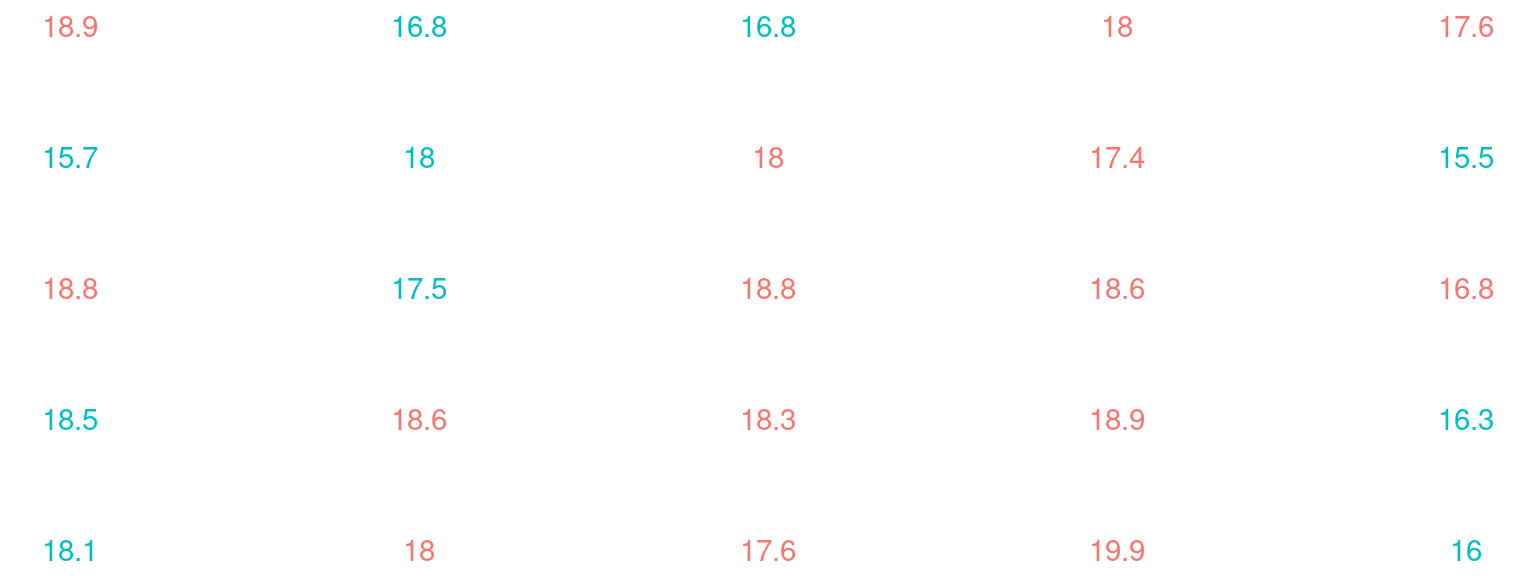
\includegraphics{C01_prelim_files/figure-pdf/unnamed-chunk-2-1.pdf}

}

\caption{Figura 1: Edades de 100 personas coloreadas por género, siendo
femeninos los rojos y masculinos los azules. Fuente: elaboración propia
a partir de simulación.}

\end{figure}%

Esta forma de ver los datos no nos entrega una información fácil de
comprender. Por esta razón, la \textbf{visualización de datos} es
importante en el análisis estadístico. Para comprender mejor, abordemos
primero la edad. Podemos ver los datos de la edad como puntos en el eje
horizontal.

\begin{figure}[H]

{\centering 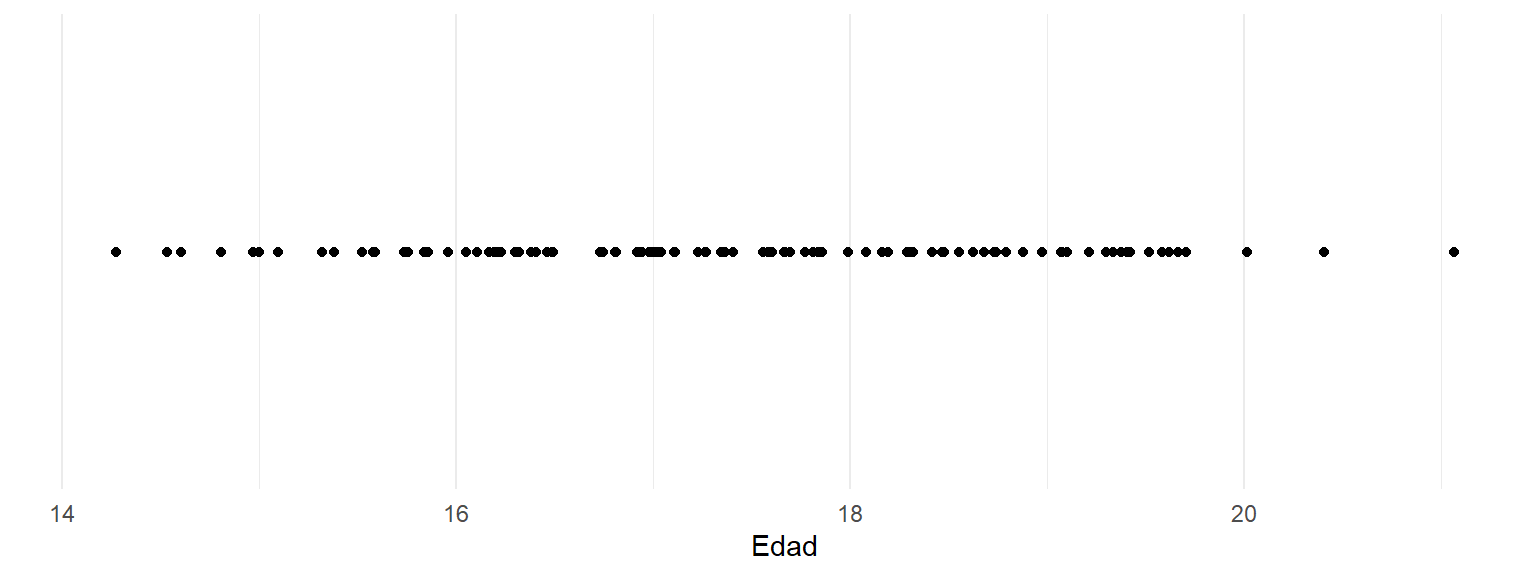
\includegraphics{C01_prelim_files/figure-pdf/unnamed-chunk-3-1.pdf}

}

\caption{Figura 2: Edades de 100 personas en el eje horizontal. Fuente:
elaboración propia a partir de simulación.}

\end{figure}%

Esta visualización nos entrega un poco más de información, podemos
entender el valor más alto, el más bajo, y en general el espacio que
ocupan los datos en el eje horizontal. Los datos que ocupan mucho
espacio se llaman \textbf{dispersos}, si el espacio es poco, se llaman
\textbf{concentrados}. Más adelante veremos medidas para esta
característica y profundizaremos al respecto. Para verlos mejor, podemos
diseminarlos verticalmente. Este es un truco que ayuda a comprender
mejor los datos, impidiendo que se sobrepongan los puntos. Para esto se
agrega ruido en el eje vertical, pero este ruido no tiene significado.

\begin{figure}[H]

{\centering \includegraphics{C01_prelim_files/figure-pdf/unnamed-chunk-4-1.pdf}

}

\caption{Figura 3: Edades de 100 personas en el eje horizontal con ruido
vertical. Fuente: elaboración propia a partir de simulación.}

\end{figure}%

Podemos trazar líneas imaginarias para entender mejor los datos. Las
primeras líneas imaginarias son el máximo y el mínimo. Al trazar estas
líneas podemos contener el 100\% de los datos. Es muy fácil.

\begin{figure}[H]

{\centering 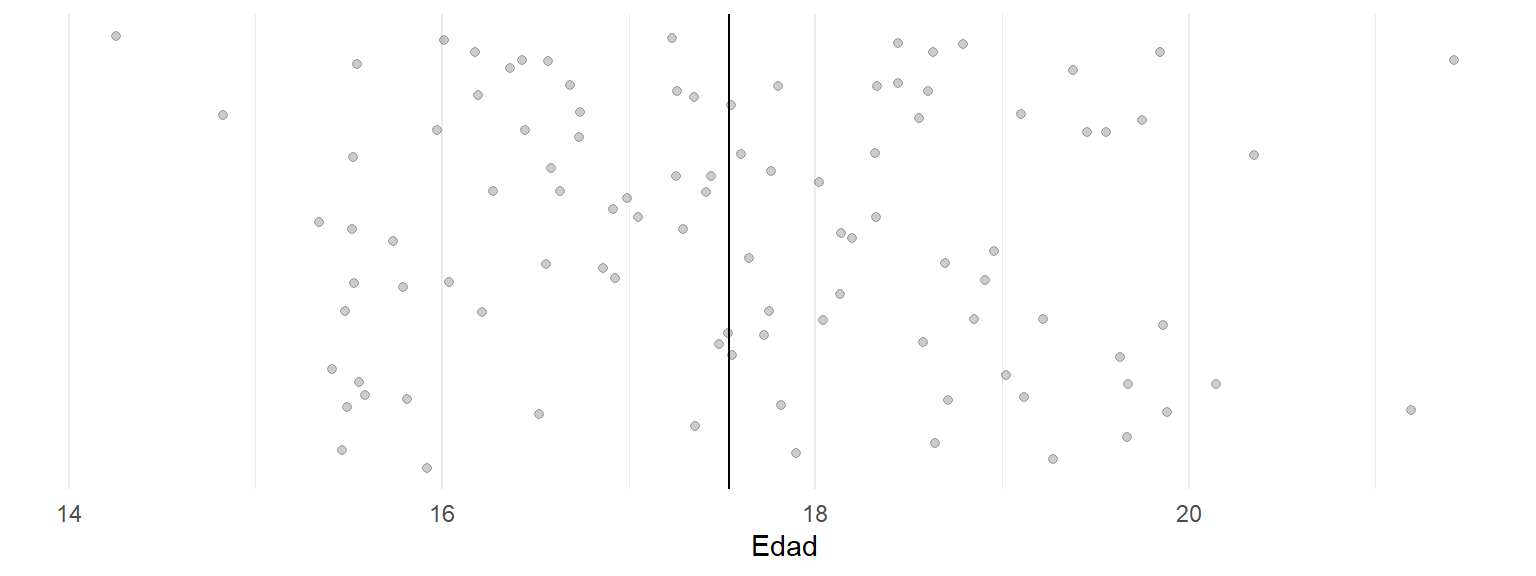
\includegraphics{C01_prelim_files/figure-pdf/unnamed-chunk-5-1.pdf}

}

\caption{Figura 4: Edades de 100 personas en el eje horizontal con
máximo y mínimo. Fuente: elaboración propia a partir de simulación.}

\end{figure}%

divide los datos en dos conjuntos de igual magnitud. A la derecha de la
línea se encuentra la misma cantidad de datos que a la izquierda. Esta
línea se encuentra en un punto muy importante del eje horizontal, este
valor se denomina la mediana. La mediana de un conjunto de datos es el
valor que divide a los datos en dos conjuntos de igual magnitud.

\begin{figure}[H]

{\centering 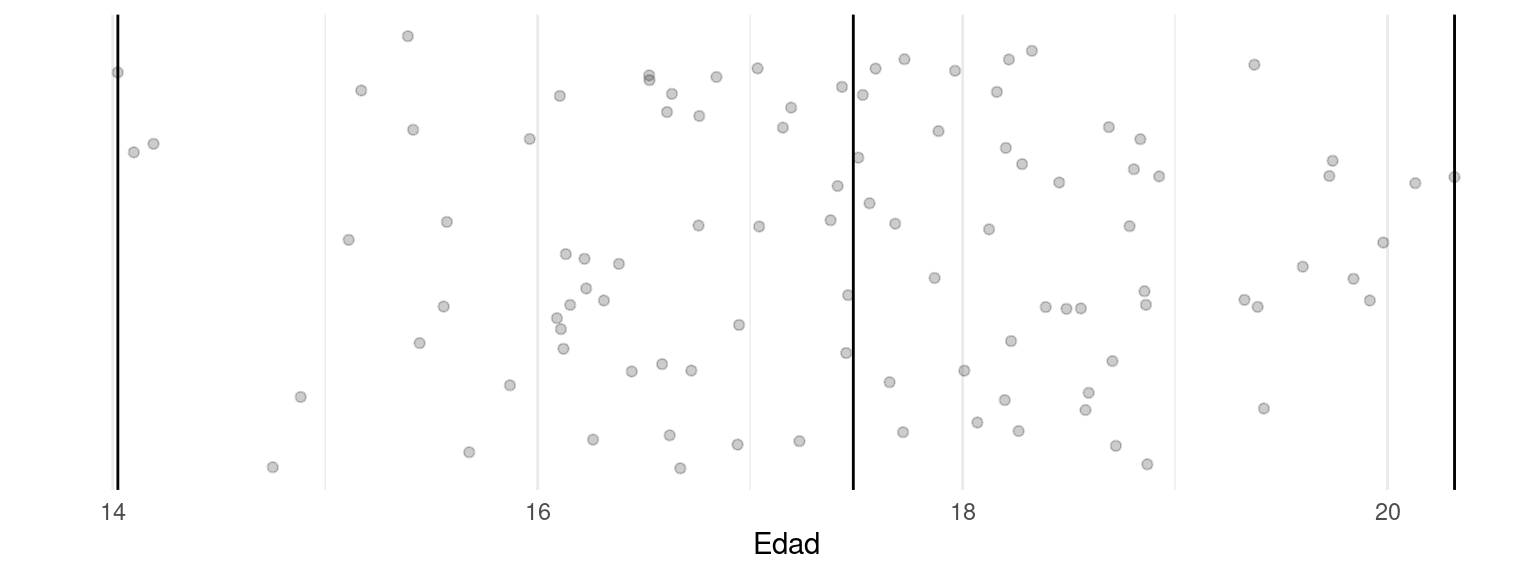
\includegraphics{C01_prelim_files/figure-pdf/unnamed-chunk-6-1.pdf}

}

\caption{Figura 5: Edades de 100 personas en el eje horizontal con su
mediana. Fuente: elaboración propia a partir de simulación.}

\end{figure}%

Usando más líneas imaginarias podemos dividirlos en cuatro partes
iguales.Estas líneas imaginarias distribuyen los datos de la edad en
cuatro conjuntos de igual magnitud. Al igual que la mediana, estos
valores son importantes. Se denominan cuartiles. En cada uno de los
conjuntos resultantes, se encuentra el 25\% de los datos.

Entonces, funciona de la siguiente forma: el cuartil cero \((Q_0)\)
corresponde al valor mínimo; el primer cuartil \((Q_1)\) separa el 25\%
de los datos; el segundo cuartil \((Q_2)\) coincide con la mediana,
porque separa el 50\% de los datos; el tercer cuartil \((Q_3)\) separa
el 75\% de los datos; y el cuarto cuartil \((Q_4)\) coincide con el
máximo de los datos.

Estos cuartiles en general no tienen la misma distancia entre ellos. Lo
usual es que se ubiquen en distancias diferentes según los datos.

\begin{figure}[H]

{\centering \includegraphics{C01_prelim_files/figure-pdf/unnamed-chunk-7-1.pdf}

}

\caption{Figura 6: Edades de 100 personas en el eje horizontal con
cuartiles. Fuente: elaboración propia a partir de simulación.}

\end{figure}%

Estas líneas imaginarias que son importantes, se pueden consolidar en un
solo gráfico, que se denomina gráfico de caja y bigotes. Este gráfico
está conformado por la mediana y los cuartiles. Este es un gráfico
escencial en el análisis de datos y lo vamos a ver en muchas
investigaciones.

Este gráfico tiene un cambio con respecto a la construcción anterior:
aquí se utilizan un máximo teórico y un mínimo teórico. Esto se realiza
con el fin de identificar visualmente los datos de los extremos.

\begin{figure}[H]

{\centering 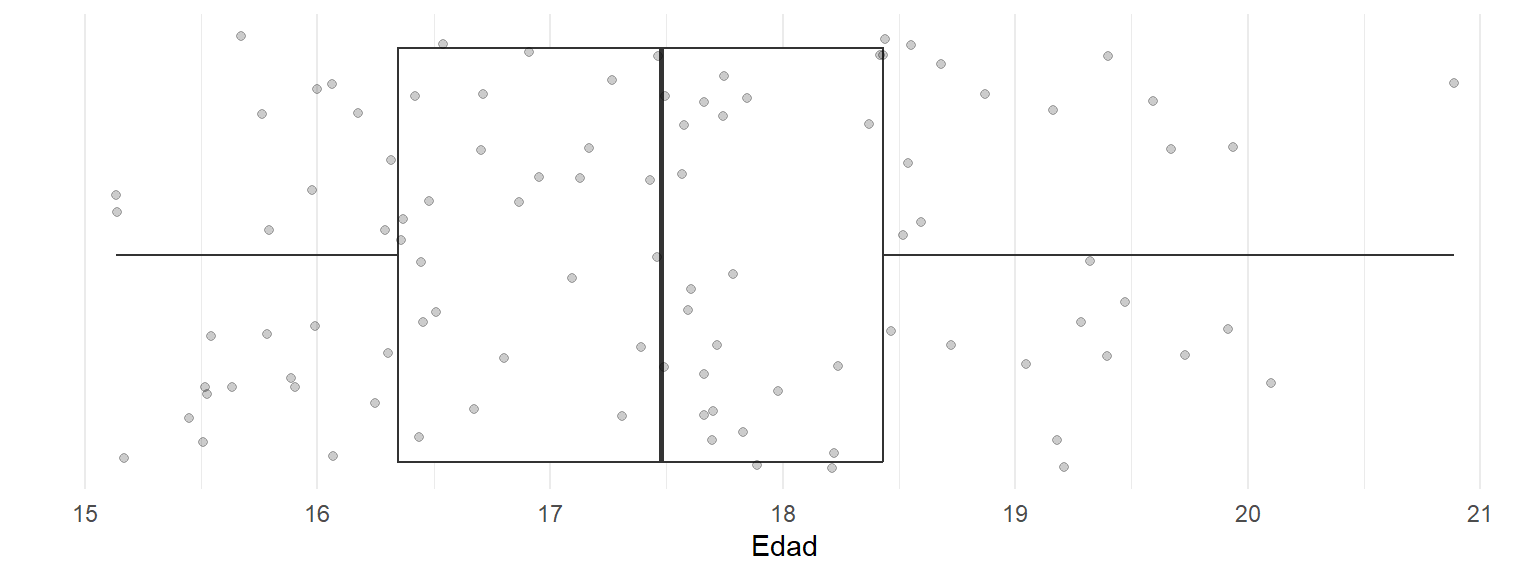
\includegraphics{C01_prelim_files/figure-pdf/unnamed-chunk-8-1.pdf}

}

\caption{Figura 7: Edades de 100 personas, gráfico de caja y bigotes.
Fuente: elaboración propia a partir de simulación.}

\end{figure}%

Abordemos el género ahora. Podemos usar el color para identificar el
género en los datos. Realizamos el mismo procedimiento añadiendo el
color del género. En este caso, ya podemos identificar la tendencia, de
puntos rojos más a la derecha y azules a la izquierda.

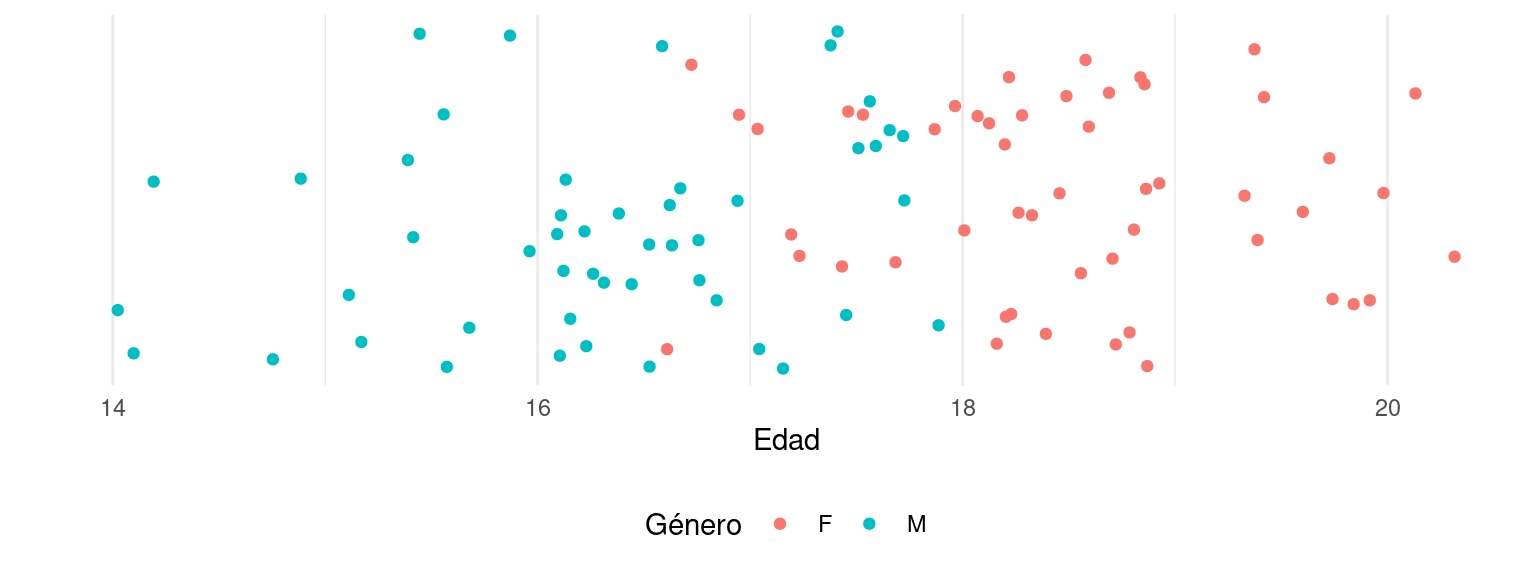
\includegraphics{C01_prelim_files/figure-pdf/unnamed-chunk-9-1.pdf}

Organizamos los datos verticalemnte por género. Esto os permite tenre
dos nubes de puntos y facilita la interpretación, ahora es más notoria
la tendencia hacia a la derecha y hacia la izquerda de los puntos rojos
y azules respectivamente.

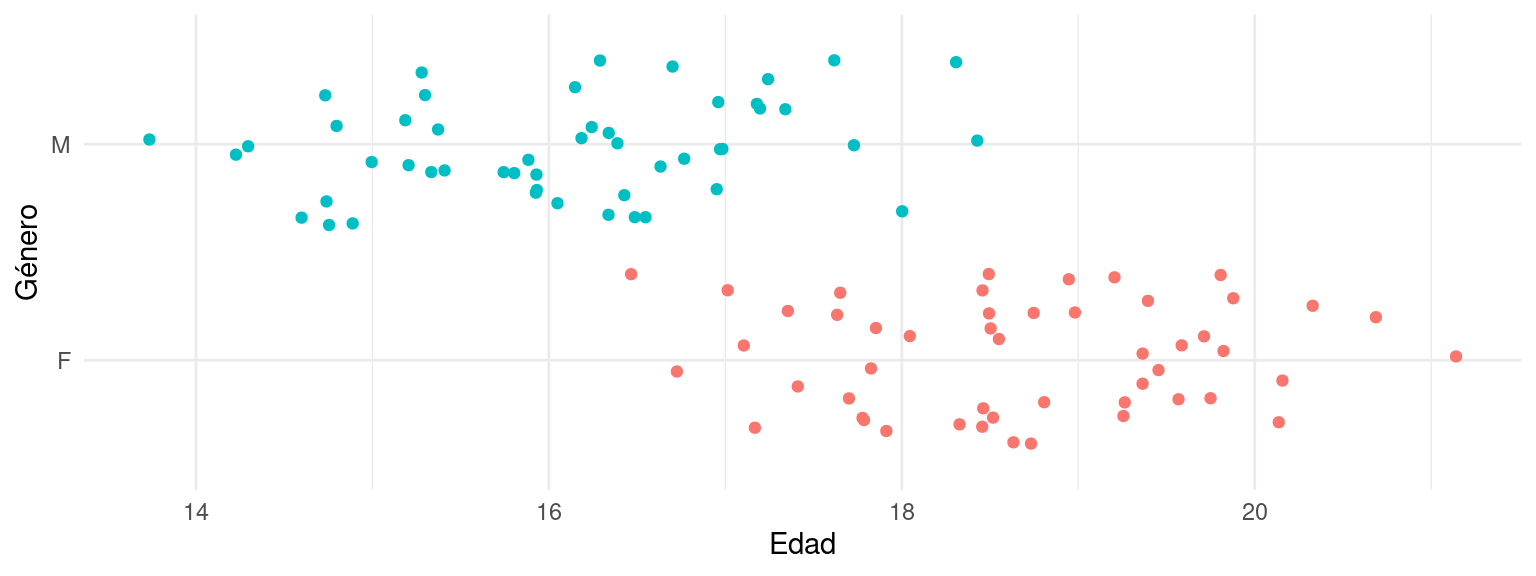
\includegraphics{C01_prelim_files/figure-pdf/unnamed-chunk-10-1.pdf}

Al elaborar una gráfico de caja para cada género es posible ver la
tendencia. Esta característica que no resultaba fácil de identificar en
el primer gráfico, ahora es muy notoria. Las medianas y los cuartiles de
los datos agrupados por género difieren. Esto nos permite obtener
hipótesis que podremos comprobar más adelante.

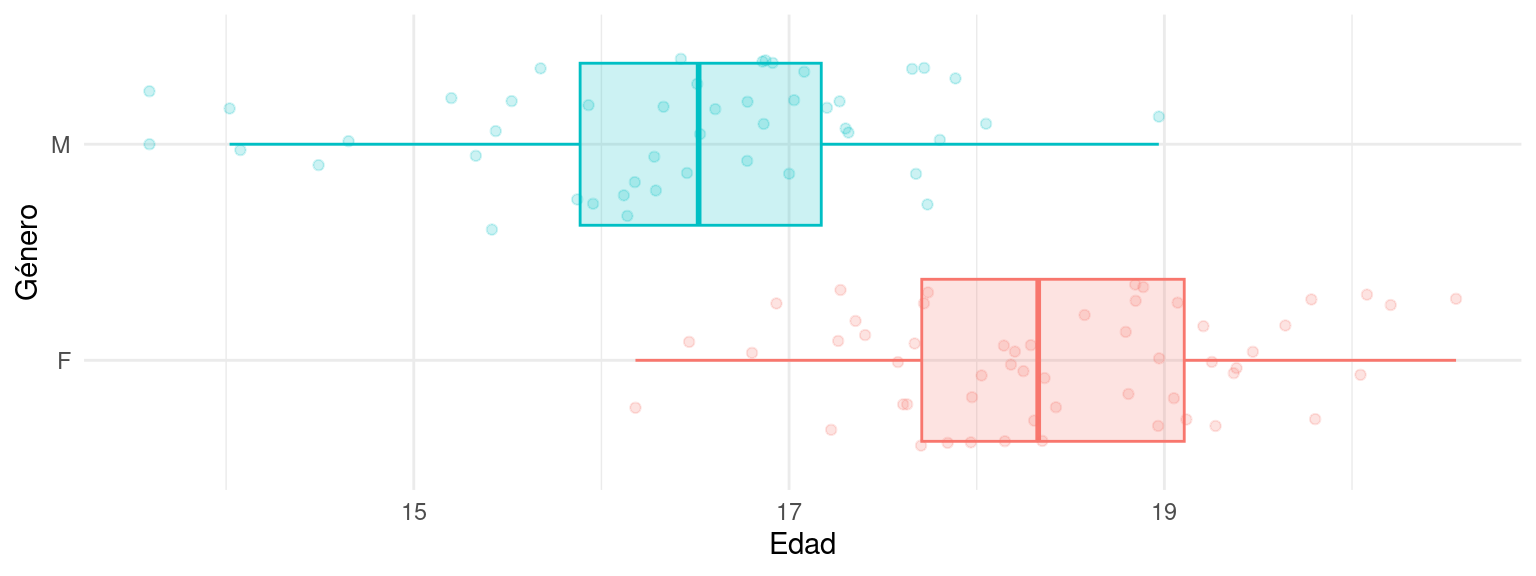
\includegraphics{C01_prelim_files/figure-pdf/unnamed-chunk-11-1.pdf}

\section{Tipos de datos}\label{tipos-de-datos}

El análisis de datos es la columna vertebral de la investigación
científica y social, donde se busca extraer patrones, relaciones y
tendencias a partir de observaciones sistemáticas. Los datos son el
insumo principal de este análisis, y comprender sus diferentes tipos y
propiedades es esencial para elegir las metodologías y enfoques más
adecuados. A continuación, se profundiza en los conceptos clave
presentados, estructurándolos en torno a su relevancia en la
investigación.

\subsection{Tendencias y patrones
globales}\label{tendencias-y-patrones-globales}

Las tendencias representan comportamientos agregados que emergen de las
características individuales de una población. A diferencia de una
afirmación puntual o específica sobre un individuo, las tendencias
buscan capturar patrones generalizables que describen cómo un grupo, en
promedio, se comporta respecto a una variable o conjunto de variables.
Este enfoque es crucial en disciplinas como la economía, la sociología y
la epidemiología, donde los fenómenos globales informan decisiones de
política pública o estrategias organizacionales.

Por ejemplo, al analizar los hábitos de consumo en un país, una
tendencia podría revelar que el promedio de gasto en entretenimiento es
más alto en grupos jóvenes que en mayores de 50 años. Sin embargo, esta
tendencia no asegura que todos los jóvenes gasten más en
entretenimiento, sino que describe un comportamiento predominante dentro
de la población estudiada. Este desajuste entre las tendencias y los
comportamientos individuales resalta la importancia de interpretar los
datos globales como representativos, pero no absolutos.

\subsection{Unidades de análisis}\label{unidades-de-anuxe1lisis}

Los individuos son las unidades básicas de observación en cualquier
estudio. Representan los elementos de la población objeto de análisis,
que pueden ser personas, empresas, organismos o eventos, dependiendo del
contexto de la investigación. En términos analíticos, los individuos son
la fuente de datos a partir de los cuales se construyen modelos,
hipótesis y conclusiones.

La elección de los individuos y su caracterización es clave, ya que
determina la validez y generalizabilidad de los resultados. Por ejemplo,
en un estudio sobre hábitos alimenticios, seleccionar individuos
representativos de diferentes regiones y estratos socioeconómicos
garantizará que las conclusiones puedan extrapolarse al resto de la
población. Este concepto está íntimamente ligado al diseño del muestreo
y la operacionalización de las variables.

\section{Variables: Características observables y
medibles}\label{variables-caracteruxedsticas-observables-y-medibles}

Las variables son los rasgos o atributos que describen a los individuos
y sobre los cuales se recopila información. Funcionan como el puente
entre las observaciones individuales y los análisis que buscan
generalizar comportamientos.

\subsection{Clasificación de las
variables}\label{clasificaciuxf3n-de-las-variables}

\begin{enumerate}
\def\labelenumi{\arabic{enumi}.}
\item
  \textbf{Cuantitativas}: Estas variables representan magnitudes
  numéricas que se pueden medir. Por otro lado, las variables numéricas
  o cuantitativas permiten medir y realizar cálculos matemáticos. La
  distinción entre discretas y continuas tiene implicaciones
  metodológicas: mientras que las discretas suelen analizarse con
  conteos y proporciones, las continuas requieren herramientas que
  consideren distribuciones más complejas. Estas variables son
  esenciales en áreas como la economía y la biología, donde los
  fenómenos físicos y financieros se representan mediante medidas
  precisas.

  \begin{itemize}
  \item
    \textbf{Discretas}: Toman valores finitos o contables, como el
    número de hijos en una familia.
  \item
    \textbf{Continuas}: Admiten infinitos valores dentro de un rango,
    como la temperatura medida en grados Celsius.
  \end{itemize}
\item
  \textbf{Categóricas}: Representan atributos o categorías que no
  necesariamente poseen un valor numérico. Las variables categóricas
  agrupan a los individuos en categorías o clases. Su análisis permite
  identificar frecuencias y distribuciones dentro de la población. Por
  ejemplo, analizar la afiliación política de un grupo puede mostrar que
  el 40\% prefiere un partido A, mientras que el 30\% opta por un
  partido B. Este tipo de variable es fundamental en estudios
  demográficos y de percepción social, donde las características
  subjetivas y de identidad son el foco principal.

  \begin{itemize}
  \tightlist
  \item
    \textbf{Nominales}: Categorías sin orden intrínseco, como el color
    de los ojos o el estado civil.\\
  \item
    \textbf{Ordinales}: Categorías con un orden lógico, como los niveles
    educativos o el nivel de satisfacción.
  \end{itemize}
\end{enumerate}

\subsection{Medición: Asignación de valores a las
observaciones}\label{mediciuxf3n-asignaciuxf3n-de-valores-a-las-observaciones}

La medición es el proceso mediante el cual las características de los
individuos se transforman en datos observables y cuantificables. Este
proceso debe ser riguroso y consistente, basado en reglas
preestablecidas que garanticen la comparabilidad y la reproducibilidad
de los resultados.

Por ejemplo, en un estudio sobre bienestar subjetivo, es esencial que
las escalas utilizadas para medir ``felicidad'' o ``satisfacción'' estén
claramente definidas, estandarizadas y validadas. Una medición precisa y
confiable no solo facilita el análisis estadístico, sino que también
asegura que las conclusiones se basen en datos sólidos y significativos.

Los tipos de datos, las variables y las técnicas de medición constituyen
los elementos centrales del análisis en cualquier disciplina. Entender
cómo se relacionan las tendencias globales con las características
individuales, cómo se seleccionan y clasifican las variables, y cómo se
mide con precisión cada atributo son habilidades fundamentales para el
análisis riguroso. Este marco integrado no solo es esencial para la
investigación académica, sino también para la toma de decisiones
informadas en contextos profesionales y sociales. La reconceptualización
del trabajo con datos requiere, por tanto, no solo conocimiento técnico,
sino también una reflexión crítica sobre las implicaciones de cómo
estructuramos y utilizamos la información.

\chapter{Preparación de los datos}\label{preparaciuxf3n-de-los-datos}

\section{Imputación de datos}\label{imputaciuxf3n-de-datos}

\section{Identificación de
atípicos}\label{identificaciuxf3n-de-atuxedpicos}

\section{De categórico a numérico}\label{de-categuxf3rico-a-numuxe9rico}

\section{De numérico a categórico}\label{de-numuxe9rico-a-categuxf3rico}

\section{Trabajo con fechas}\label{trabajo-con-fechas}

\chapter{Estadística descriptiva para una
variable}\label{estaduxedstica-descriptiva-para-una-variable-1}

\section{Medidas de frecuencia}\label{medidas-de-frecuencia}

En el análisis de datos dentro de las ciencias sociales, las medidas de
frecuencia permiten describir de manera precisa la distribución de
variables \textbf{categóricas} y ayudan a comprender patrones generales
en poblaciones o muestras. Estas medidas son esenciales para resumir y
comunicar la información de forma efectiva, aportando una base sólida
para el análisis estadístico posterior.

\subsection{Frecuencia}\label{frecuencia}

La \textbf{frecuencia absoluta} es el conteo del número de veces que
aparece una categoría específica en un conjunto de datos. Es la medida
más básica de estadística descriptiva y es crucial para comprender la
distribución de variables cualitativas. Las categorías en un conjunto de
datos representan respuestas a preguntas de encuestas, atributos de los
participantes o clasificaciones en estudios sociales.

\begin{tcolorbox}[enhanced jigsaw, toprule=.15mm, opacitybacktitle=0.6, toptitle=1mm, arc=.35mm, left=2mm, title=\textcolor{quarto-callout-tip-color}{\faLightbulb}\hspace{0.5em}{Tip}, titlerule=0mm, leftrule=.75mm, rightrule=.15mm, coltitle=black, bottomtitle=1mm, bottomrule=.15mm, colframe=quarto-callout-tip-color-frame, opacityback=0, colback=white, breakable, colbacktitle=quarto-callout-tip-color!10!white]

\textbf{Ejemplo aplicado a las ciencias sociales}: En un estudio sobre
preferencias políticas, los encuestados pueden expresar su afinidad por
diferentes partidos. Si en una muestra de 500 personas, 150 apoyan el
partido A, 200 el partido B y 150 no apoyan a ningún partido, la
frecuencia de cada categoría sería:

\begin{itemize}
\tightlist
\item
  \textbf{Partido A}: 150
\item
  \textbf{Partido B}: 200
\item
  \textbf{Ninguno}: 150
\end{itemize}

Este conteo ayuda a determinar cuál es el partido con mayor número de
seguidores y, por ende, cuál tiene una posición predominante en la
muestra.

\end{tcolorbox}

\subsection{Proporción}\label{proporciuxf3n}

La \textbf{proporción} se utiliza para expresar la frecuencia relativa
de una categoría con respecto al total de observaciones, facilitando la
comparación entre diferentes grupos de datos. Se calcula dividiendo la
frecuencia de una categoría por el total de observaciones.

\begin{tcolorbox}[enhanced jigsaw, toprule=.15mm, opacitybacktitle=0.6, toptitle=1mm, arc=.35mm, left=2mm, title=\textcolor{quarto-callout-warning-color}{\faExclamationTriangle}\hspace{0.5em}{Warning}, titlerule=0mm, leftrule=.75mm, rightrule=.15mm, coltitle=black, bottomtitle=1mm, bottomrule=.15mm, colframe=quarto-callout-warning-color-frame, opacityback=0, colback=white, breakable, colbacktitle=quarto-callout-warning-color!10!white]

\textbf{Fórmula:}

\[p_i = \frac{\#\text{freq}_i}{n}\]

Donde:

\begin{itemize}
\tightlist
\item
  \(p_i\) es la proporción.
\item
  \(\#\text{freq}_i\) es la frecuencia de la categoría específica
  (\(i\)-ésima).
\item
  \(n\) es el número total de observaciones.
\end{itemize}

\end{tcolorbox}

\begin{tcolorbox}[enhanced jigsaw, toprule=.15mm, opacitybacktitle=0.6, toptitle=1mm, arc=.35mm, left=2mm, title=\textcolor{quarto-callout-tip-color}{\faLightbulb}\hspace{0.5em}{Tip}, titlerule=0mm, leftrule=.75mm, rightrule=.15mm, coltitle=black, bottomtitle=1mm, bottomrule=.15mm, colframe=quarto-callout-tip-color-frame, opacityback=0, colback=white, breakable, colbacktitle=quarto-callout-tip-color!10!white]

\textbf{Ejemplo contextualizado}: Supongamos que en una encuesta sobre
el uso de redes sociales, se encontró que 320 de 800 personas utilizan
redes sociales diariamente. La proporción de usuarios diarios es:

\[p_{rs} = \frac{320}{800} = 0.40 \text{ o } 40\%\]

Este resultado indica que el 40\% de los encuestados son usuarios
diarios de redes sociales, un hallazgo importante para estudios sobre
comportamiento digital y hábitos de consumo en la sociedad.

\end{tcolorbox}

Las frecuencias relativas suelen presentarse en porcentajes. Un
\textbf{porcentaje} es una forma de expresar una fracción o proporción
sobre un total de 100, facilitando la comparación y comprensión de datos
en contextos variados. Se utiliza ampliamente en estadísticas, finanzas
y análisis cuantitativo para representar partes de un todo. La palabra
``porcentaje'' proviene del latín ``per centum,'' que significa ``por
cada cien.'' Su uso se remonta a la antigua Roma, donde los comerciantes
y cobradores de impuestos empleaban fracciones y cálculos semejantes al
porcentaje moderno para facilitar transacciones y registros contables. A
lo largo de los siglos, el concepto se perfeccionó, especialmente
durante el Renacimiento, con la expansión del comercio y la necesidad de
representar proporciones de forma estandarizada, llevando al símbolo
``\%'' que hoy es universal.

\subsection{Moda}\label{moda}

La \textbf{moda} es la categoría con mayor frecuencia en un conjunto de
datos y representa el valor más común o frecuente. Esta medida es
particularmente útil en estudios sociales cuando se analizan
características como la ocupación, el nivel de estudios o las opiniones
sobre políticas públicas. La moda permite identificar tendencias
dominantes o respuestas mayoritarias en la población estudiada.

\begin{tcolorbox}[enhanced jigsaw, toprule=.15mm, opacitybacktitle=0.6, toptitle=1mm, arc=.35mm, left=2mm, title=\textcolor{quarto-callout-tip-color}{\faLightbulb}\hspace{0.5em}{Tip}, titlerule=0mm, leftrule=.75mm, rightrule=.15mm, coltitle=black, bottomtitle=1mm, bottomrule=.15mm, colframe=quarto-callout-tip-color-frame, opacityback=0, colback=white, breakable, colbacktitle=quarto-callout-tip-color!10!white]

\textbf{Ejemplo aplicado}: Imaginemos un estudio que investiga la
ocupación principal de los trabajadores en una ciudad. Si los datos
muestran que, de 1,000 encuestados, 450 trabajan en el sector servicios,
300 en el sector manufacturero y 250 en el sector tecnológico. En este
caso la moda es ``Sector servicios''

Este dato resalta que la ocupación predominante en la muestra es el
sector servicios, una observación relevante para estudios de desarrollo
económico y planificación urbana.

\end{tcolorbox}

\subsection{Nota sobre variables
continuas}\label{nota-sobre-variables-continuas}

La moda tiene aplicaciones limitadas en variables continuas, como el
ingreso o la altura, ya que estas tienden a no repetir valores exactos
con frecuencia significativa. Sin embargo, en ciertas investigaciones
sociales, agrupar datos en rangos puede hacer que la moda sea más útil.
Por ejemplo, si se clasifica el ingreso en intervalos como ``menos de
\$10,000'', ``\$10,001-\$20,000'',\ldots, etc., puede ser posible
identificar una moda representativa del grupo con mayor frecuencia.

\begin{tcolorbox}[enhanced jigsaw, toprule=.15mm, opacitybacktitle=0.6, toptitle=1mm, arc=.35mm, left=2mm, title=\textcolor{quarto-callout-tip-color}{\faLightbulb}\hspace{0.5em}{Tip}, titlerule=0mm, leftrule=.75mm, rightrule=.15mm, coltitle=black, bottomtitle=1mm, bottomrule=.15mm, colframe=quarto-callout-tip-color-frame, opacityback=0, colback=white, breakable, colbacktitle=quarto-callout-tip-color!10!white]

\textbf{Ejemplo adaptado}: Si se analizan los ingresos de 500 hogares y
el intervalo ``\$10,001-\$20,000'' tiene la mayor cantidad de hogares
(150), entonces la moda del ingreso agrupado es ese intervalo
específico. Esta información puede ser crucial para entender el nivel
socioeconómico predominante en un área geográfica y para la formulación
de políticas de asistencia económica.

\end{tcolorbox}

\section{Medidas de tendencia
central}\label{medidas-de-tendencia-central}

Las \textbf{medidas de tendencia central} son estadísticas descriptivas
que representan el valor típico o central de un conjunto de datos. Estas
medidas permiten comprender dónde se encuentra el ``centro'' de una
distribución y son fundamentales en la investigación cuantitativa en
ciencias sociales, donde se estudian fenómenos como ingresos, opiniones
o resultados de encuestas.

\subsection{Media aritmética}\label{media-aritmuxe9tica}

La \textbf{media aritmética}, comúnmente conocida como promedio, es la
medida de tendencia central más utilizada. Se obtiene sumando todos los
valores de un conjunto de datos y dividiendo el resultado por el número
total de observaciones. La media es ideal para describir conjuntos de
datos simétricos y es especialmente útil en estudios de ciencias
sociales cuando se necesita resumir características cuantitativas como
la edad, el ingreso o la puntuación de una encuesta.

\begin{tcolorbox}[enhanced jigsaw, toprule=.15mm, opacitybacktitle=0.6, toptitle=1mm, arc=.35mm, left=2mm, title=\textcolor{quarto-callout-warning-color}{\faExclamationTriangle}\hspace{0.5em}{Warning}, titlerule=0mm, leftrule=.75mm, rightrule=.15mm, coltitle=black, bottomtitle=1mm, bottomrule=.15mm, colframe=quarto-callout-warning-color-frame, opacityback=0, colback=white, breakable, colbacktitle=quarto-callout-warning-color!10!white]

\textbf{Fórmula de la media:}
\[\overline{x} = \frac{1}{n} \sum_{i=1}^{n} x_i\]

Donde:

\begin{itemize}
\tightlist
\item
  \(\overline{x}\) es la media,
\item
  \(n\) es el número de observaciones,
\item
  \(x_i\) representa cada valor individual del conjunto de datos.
\end{itemize}

\end{tcolorbox}

\begin{tcolorbox}[enhanced jigsaw, toprule=.15mm, opacitybacktitle=0.6, toptitle=1mm, arc=.35mm, left=2mm, title=\textcolor{quarto-callout-tip-color}{\faLightbulb}\hspace{0.5em}{Tip}, titlerule=0mm, leftrule=.75mm, rightrule=.15mm, coltitle=black, bottomtitle=1mm, bottomrule=.15mm, colframe=quarto-callout-tip-color-frame, opacityback=0, colback=white, breakable, colbacktitle=quarto-callout-tip-color!10!white]

\textbf{Ejemplo en ciencias sociales}: Supongamos que estamos estudiando
los ingresos mensuales en una comunidad y los datos obtenidos en dólares
son: 1,200, 1,500, 1,800, 2,000 y 20,000. La media de estos ingresos es:

\[\overline{x} = \frac{1,200 + 1,500 + 1,800 + 2,000 + 20,000}{5} = \frac{26,500}{5} = 5,300\]

Aunque la media es 5,300, este valor puede no representar adecuadamente
la distribución, ya que un ingreso atípico de 20,000 distorsiona el
promedio.

\end{tcolorbox}

\subsection{Mediana}\label{mediana}

La \textbf{mediana} es la medida de tendencia central que divide un
conjunto de datos ordenados en dos partes iguales, es decir, la mitad de
los datos está por debajo y la otra mitad por encima de la mediana. Esta
medida es más resistente a los valores extremos que la media, por lo que
es preferida en distribuciones sesgadas o con outliers.

\begin{tcolorbox}[enhanced jigsaw, toprule=.15mm, opacitybacktitle=0.6, toptitle=1mm, arc=.35mm, left=2mm, title=\textcolor{quarto-callout-tip-color}{\faLightbulb}\hspace{0.5em}{Tip}, titlerule=0mm, leftrule=.75mm, rightrule=.15mm, coltitle=black, bottomtitle=1mm, bottomrule=.15mm, colframe=quarto-callout-tip-color-frame, opacityback=0, colback=white, breakable, colbacktitle=quarto-callout-tip-color!10!white]

\textbf{Procedimiento para encontrar la mediana}:

\begin{itemize}
\tightlist
\item
  Si el número de observaciones es impar, la mediana es el valor
  central.
\item
  Si es par, la mediana es el promedio de los dos valores centrales.
\end{itemize}

\end{tcolorbox}

\begin{tcolorbox}[enhanced jigsaw, toprule=.15mm, opacitybacktitle=0.6, toptitle=1mm, arc=.35mm, left=2mm, title=\textcolor{quarto-callout-tip-color}{\faLightbulb}\hspace{0.5em}{Tip}, titlerule=0mm, leftrule=.75mm, rightrule=.15mm, coltitle=black, bottomtitle=1mm, bottomrule=.15mm, colframe=quarto-callout-tip-color-frame, opacityback=0, colback=white, breakable, colbacktitle=quarto-callout-tip-color!10!white]

\textbf{Ejemplo aplicado}: Si analizamos el número de hijos en familias
de una comunidad y los datos ordenados son: 1, 2, 2, 3 y 10, la mediana
es 2, ya que es el valor del medio.

\end{tcolorbox}

\subsection{Otras medidas de tendencia
central}\label{otras-medidas-de-tendencia-central}

\subsubsection{Media armónica}\label{media-armuxf3nica}

La \textbf{media armónica} es útil para conjuntos de datos que
representan tasas o razones, ya que pondera los valores de forma que las
observaciones más pequeñas tengan un mayor impacto. Se define como el
inverso del promedio de los inversos de los valores.

\begin{tcolorbox}[enhanced jigsaw, toprule=.15mm, opacitybacktitle=0.6, toptitle=1mm, arc=.35mm, left=2mm, title=\textcolor{quarto-callout-warning-color}{\faExclamationTriangle}\hspace{0.5em}{Warning}, titlerule=0mm, leftrule=.75mm, rightrule=.15mm, coltitle=black, bottomtitle=1mm, bottomrule=.15mm, colframe=quarto-callout-warning-color-frame, opacityback=0, colback=white, breakable, colbacktitle=quarto-callout-warning-color!10!white]

\textbf{Fórmula de la media armónica:}

\[\overline{x}_{\text{arm}} = \frac{n}{\sum_{i=1}^{n} \frac{1}{x_i}}\]

Donde:

\end{tcolorbox}

\begin{tcolorbox}[enhanced jigsaw, toprule=.15mm, opacitybacktitle=0.6, toptitle=1mm, arc=.35mm, left=2mm, title=\textcolor{quarto-callout-tip-color}{\faLightbulb}\hspace{0.5em}{Tip}, titlerule=0mm, leftrule=.75mm, rightrule=.15mm, coltitle=black, bottomtitle=1mm, bottomrule=.15mm, colframe=quarto-callout-tip-color-frame, opacityback=0, colback=white, breakable, colbacktitle=quarto-callout-tip-color!10!white]

\textbf{Ejemplo en ciencias sociales}: Supongamos que estudiamos la
eficiencia de diferentes métodos de transporte urbano en términos de
tiempo por viaje. Si los tiempos por viaje (en minutos) son 10, 15 y 20,
la media armónica es:

\[\overline{x}_{\text{arm}} = \frac{3}{\frac{1}{10} + \frac{1}{15} + \frac{1}{20}} \approx 13.04\]
Esta media pondera más los viajes cortos y es útil en análisis donde las
tasas individuales son significativas.

\end{tcolorbox}

\subsubsection{Media geométrica}\label{media-geomuxe9trica}

La \textbf{media geométrica} es apropiada para datos que representan
crecimiento proporcional o tasas de cambio, como el crecimiento de la
población o el rendimiento económico. Es el ( n )-ésimo raíz del
producto de todos los valores.

\begin{tcolorbox}[enhanced jigsaw, toprule=.15mm, opacitybacktitle=0.6, toptitle=1mm, arc=.35mm, left=2mm, title=\textcolor{quarto-callout-warning-color}{\faExclamationTriangle}\hspace{0.5em}{Warning}, titlerule=0mm, leftrule=.75mm, rightrule=.15mm, coltitle=black, bottomtitle=1mm, bottomrule=.15mm, colframe=quarto-callout-warning-color-frame, opacityback=0, colback=white, breakable, colbacktitle=quarto-callout-warning-color!10!white]

\textbf{Fórmula de la media geométrica:}

\[\overline{x}_{\text{geo}} = \sqrt[n]{x_1 \cdot x_2 \cdot \ldots \cdot x_n}\]

\end{tcolorbox}

\begin{tcolorbox}[enhanced jigsaw, toprule=.15mm, opacitybacktitle=0.6, toptitle=1mm, arc=.35mm, left=2mm, title=\textcolor{quarto-callout-tip-color}{\faLightbulb}\hspace{0.5em}{Tip}, titlerule=0mm, leftrule=.75mm, rightrule=.15mm, coltitle=black, bottomtitle=1mm, bottomrule=.15mm, colframe=quarto-callout-tip-color-frame, opacityback=0, colback=white, breakable, colbacktitle=quarto-callout-tip-color!10!white]

\textbf{Ejemplo en ciencias sociales}: Si una población crece anualmente
a tasas de 1.05, 1.10 y 1.08, la media geométrica del crecimiento es:

\[\overline{x}_{\text{geo}} = \sqrt[3]{1.05 \times 1.10 \times 1.08} \approx 1.076\]

Lo que implica un crecimiento promedio anual del 7.6\%.

\end{tcolorbox}

\subsubsection{Comparación de las
medidas}\label{comparaciuxf3n-de-las-medidas}

En resumen, la \textbf{media aritmética} es ideal para datos simétricos
y sin valores extremos, la \textbf{mediana} es preferible en
distribuciones sesgadas o con valores atípicos, y las \textbf{medias
armónica y geométrica} se utilizan en contextos específicos relacionados
con tasas o datos multiplicativos. Estas medidas permiten a los
investigadores de las ciencias sociales interpretar adecuadamente los
datos y tomar decisiones basadas en análisis cuantitativos sólidos.

\section{Medidas de localización}\label{medidas-de-localizaciuxf3n}

\subsection{Mínimo y máximo}\label{muxednimo-y-muxe1ximo}

El mínimo es el valor más bajo en el conjunto de datos y el máximo es el
valor más alto. En estudios sociales, pueden utilizarse para detectar
posibles extremos en las variables, como el ingreso o la edad.

\subsection{Cuantiles}\label{cuantiles}

Los cuantiles dividen los datos en partes iguales. En estudios sociales,
los cuantiles son útiles para evaluar la distribución de ingresos o
educación. Por ejemplo, el cuartil más bajo (25\%) representa el grupo
con los ingresos más bajos.

\begin{tcolorbox}[enhanced jigsaw, toprule=.15mm, opacitybacktitle=0.6, toptitle=1mm, arc=.35mm, left=2mm, title=\textcolor{quarto-callout-warning-color}{\faExclamationTriangle}\hspace{0.5em}{Warning}, titlerule=0mm, leftrule=.75mm, rightrule=.15mm, coltitle=black, bottomtitle=1mm, bottomrule=.15mm, colframe=quarto-callout-warning-color-frame, opacityback=0, colback=white, breakable, colbacktitle=quarto-callout-warning-color!10!white]

\[Q_\alpha(x)\sim X_{(\alpha)}\]

\end{tcolorbox}

\subsection{Percentiles}\label{percentiles}

Los percentiles son un caso especial de cuantiles y se usan para ver la
posición de un valor dentro de una distribución. En educación, el
percentil 90 indica que un estudiante superó al 90\% de sus compañeros
en una prueba estandarizada.

\subsection{Cuartiles}\label{cuartiles}

Los cuartiles dividen los datos en cuatro partes. El primer cuartil (Q1)
es el 25\% más bajo, y el tercer cuartil (Q3) es el 25\% más alto. Estos
son útiles para evaluar la dispersión de los ingresos dentro de una
población.

\section{Medidas de dispersión}\label{medidas-de-dispersiuxf3n}

\subsection{Varianza}\label{varianza}

La varianza mide qué tan dispersos están los datos respecto a la media.
En estudios de desigualdad de ingresos, una alta varianza indicaría
grandes disparidades entre los ingresos de las personas.

\begin{tcolorbox}[enhanced jigsaw, toprule=.15mm, opacitybacktitle=0.6, toptitle=1mm, arc=.35mm, left=2mm, title=\textcolor{quarto-callout-warning-color}{\faExclamationTriangle}\hspace{0.5em}{Warning}, titlerule=0mm, leftrule=.75mm, rightrule=.15mm, coltitle=black, bottomtitle=1mm, bottomrule=.15mm, colframe=quarto-callout-warning-color-frame, opacityback=0, colback=white, breakable, colbacktitle=quarto-callout-warning-color!10!white]

\[ S_x^2 =\frac{1}{n} \sum\limits_{i=1}^n (x_i-\overline{x})^2\]

\end{tcolorbox}

\begin{tcolorbox}[enhanced jigsaw, toprule=.15mm, opacitybacktitle=0.6, toptitle=1mm, arc=.35mm, left=2mm, title=\textcolor{quarto-callout-tip-color}{\faLightbulb}\hspace{0.5em}{Tip}, titlerule=0mm, leftrule=.75mm, rightrule=.15mm, coltitle=black, bottomtitle=1mm, bottomrule=.15mm, colframe=quarto-callout-tip-color-frame, opacityback=0, colback=white, breakable, colbacktitle=quarto-callout-tip-color!10!white]

Ejemplo: En una muestra de ingresos de 2000, 2500, 3000, 3500 y 4000, la
varianza nos indica cuánto se alejan estos valores de la media.

\end{tcolorbox}

\subsection{Desviación estándar}\label{desviaciuxf3n-estuxe1ndar}

La desviación estándar es la raíz cuadrada de la varianza y nos
proporciona una medida de dispersión en las mismas unidades que los
datos originales. Por ejemplo, si la desviación estándar de los ingresos
en una población es alta, indica que hay una gran variabilidad en los
ingresos.

\begin{tcolorbox}[enhanced jigsaw, toprule=.15mm, opacitybacktitle=0.6, toptitle=1mm, arc=.35mm, left=2mm, title=\textcolor{quarto-callout-warning-color}{\faExclamationTriangle}\hspace{0.5em}{Warning}, titlerule=0mm, leftrule=.75mm, rightrule=.15mm, coltitle=black, bottomtitle=1mm, bottomrule=.15mm, colframe=quarto-callout-warning-color-frame, opacityback=0, colback=white, breakable, colbacktitle=quarto-callout-warning-color!10!white]

\[ S_x =\sqrt{S_x^2}\]

\end{tcolorbox}

\subsection{Rango intercuartílico
(IQR)}\label{rango-intercuartuxedlico-iqr}

El rango intercuartílico es la diferencia entre el tercer cuartil (Q3) y
el primer cuartil (Q1). Mide la dispersión central de los datos y es
útil para evitar que los valores extremos influyan en la interpretación.

\begin{tcolorbox}[enhanced jigsaw, toprule=.15mm, opacitybacktitle=0.6, toptitle=1mm, arc=.35mm, left=2mm, title=\textcolor{quarto-callout-warning-color}{\faExclamationTriangle}\hspace{0.5em}{Warning}, titlerule=0mm, leftrule=.75mm, rightrule=.15mm, coltitle=black, bottomtitle=1mm, bottomrule=.15mm, colframe=quarto-callout-warning-color-frame, opacityback=0, colback=white, breakable, colbacktitle=quarto-callout-warning-color!10!white]

\[ran(x) = Q_{3}(x) - Q_{1}(x)\]

\end{tcolorbox}

Ejemplo: En una encuesta de satisfacción con el gobierno, el IQR podría
mostrar la variación en las respuestas del 50\% central, ignorando los
valores más extremos de descontento o satisfacción.

\subsection{Rango}\label{rango}

El rango es la diferencia entre el valor máximo y el mínimo. Aunque es
fácil de calcular, puede verse afectado por valores atípicos. Por
ejemplo, en el análisis de ingresos, el rango puede ser muy amplio si
hay pocos individuos con ingresos extremadamente altos.

\begin{tcolorbox}[enhanced jigsaw, toprule=.15mm, opacitybacktitle=0.6, toptitle=1mm, arc=.35mm, left=2mm, title=\textcolor{quarto-callout-warning-color}{\faExclamationTriangle}\hspace{0.5em}{Warning}, titlerule=0mm, leftrule=.75mm, rightrule=.15mm, coltitle=black, bottomtitle=1mm, bottomrule=.15mm, colframe=quarto-callout-warning-color-frame, opacityback=0, colback=white, breakable, colbacktitle=quarto-callout-warning-color!10!white]

\[Rango = max(x) - min(x)\]

\end{tcolorbox}

\section{Ejercicios y actividades}\label{ejercicios-y-actividades}

\subsection{Hablemos bien}\label{hablemos-bien}

No diga: la gente votó \textbf{en promedio} por el candidato X

Diga: la gente votó en \textbf{mayor proporción} por el candidato X

\subsection{Actividad}\label{actividad}

No diga:

\begin{itemize}
\item
  Esta alternativa es muy buena, nos ahorra menos dolores de cabeza
\item
  La edad promedio de los estudiantes está entre 15 y 20 años.
\item
  En total, uno de cada tres estudiantes no sabe estadística.
\end{itemize}

Analice

\begin{itemize}
\item
  Más de la mitad de los estudiantes que presentaron la prueba saber
  están por debajo del promedio del puntaje de inglés.
\item
  El 70\% de los colombianos tienen ingresos por debajo de la media.
\end{itemize}

\chapter{Correlación}\label{correlaciuxf3n}

Estadística descriptiva

\hfill\break

\begin{Shaded}
\begin{Highlighting}[]
\DocumentationTok{\#\# Reescribir bien}
\end{Highlighting}
\end{Shaded}

\chapter{Dos variables}\label{dos-variables}

Es posible medir la relación entre dos variables, pero esto depende de
qué tipo de variables son.

\begin{itemize}
\tightlist
\item
  Dos cualitativas
\item
  Dos cuantitativas
\item
  Una cuantitativa y una cualitativa
\end{itemize}

\section{Dos variables cualitativas}\label{dos-variables-cualitativas}

Para poder medir la relación entre dos variables de tipo cualitativo
usamos tablas de contingencia.

\section{Dos variables cuantitativas}\label{dos-variables-cuantitativas}

La relación entre dos variables cuantitativas puede ser medida con los
siguientes estadísticos.

\begin{itemize}
\tightlist
\item
  Covarianza
\item
  Correlación de Pearson
\item
  Correlación de Spearman
\end{itemize}

\section{Covarianza}\label{covarianza}

Covarianza entre dos variables

\[ S_{xy} = \frac{1}{n}\sum\limits_{i = 1}^n (x_i - \overline{x})(y_i - \overline{y})\]

\section{Correlación de Pearson}\label{correlaciuxf3n-de-pearson}

\[\rho_{xy} = \frac{\sum x_iy_i - n\overline{x}\overline{y}}{(n-1)S_xS_y}\]

\section{Correlación de Spearman}\label{correlaciuxf3n-de-spearman}

\[\rho = 1 - \frac{6\sum D^2}{n(n^2 - 1)}\]

donde D es la diferencia entre los correspondientes estadísticos de
orden de x - y. N es el número de parejas de datos.

\section{Una variable cualitativa y otra
cuantitativa}\label{una-variable-cualitativa-y-otra-cuantitativa}

Para medir asociación entre una variable cuantitativa y otra cualitativa
se peude desagregar la media.

\section{Correlación}\label{correlaciuxf3n-1}

¿Qué es la causalidad?

\chapter{Distribuciones}\label{distribuciones}

\chapter{Visualización}\label{visualizaciuxf3n}

Estadística descriptiva

\hfill\break

\chapter{Visualización}\label{visualizaciuxf3n-1}

Iniciamos el tema de visualización de datos con una lectura refrescante:
\href{https://culturacientifica.com/2019/04/25/graficas-para-la-ciencia-y-ciencia-para-las-graficas/}{Gráficas
para la ciencia y ciencia para las gráficas}

\section{¿Por qué visualización?}\label{por-quuxe9-visualizaciuxf3n}

\begin{itemize}
\tightlist
\item
  \href{https://en.wikipedia.org/wiki/Anscombe\%27s_quartet}{El cuarteto
  de Anscombe}
\item
  \href{https://seeing-theory.brown.edu}{Seeing theory}
\end{itemize}

\section{Veamos ejemplos}\label{veamos-ejemplos}

\begin{itemize}
\tightlist
\item
  \href{https://informationisbeautiful.net/}{Information is beautiful}
\item
  \href{https://www.gapminder.org/tools}{gapmminder}
\item
  \href{https://shiny.rstudio.com/gallery/}{shiny:}
\item
  \href{https://plot.ly/feed}{plotly}
\item
  \href{https://www.oecdbetterlifeindex.org/es/}{Beter Life Index OECD}
\item
  \href{https://www.youtube.com/watch?v=dwZ6B5kalbQ}{Top 10 Countries by
  Inflation Rate (1980-2018)}
\end{itemize}

\section{El ejemplo de Napoleón}\label{el-ejemplo-de-napoleuxf3n}

\includegraphics{index_files/mediabag/1200px-Minard.png}

Fuente:
\href{https://www.researchgate.net/publication/327579298_Data_visualization_education_using_the_storytelling_with_Minard's_figurative_map}{Data
visualization education using the storytelling with Minard's figurative
map}

\section{Gráficos tradicionales}\label{gruxe1ficos-tradicionales}

\includegraphics{index_files/mediabag/excel-chart-tools-ri.png}

\section{Escala de Cleveland y
McGill}\label{escala-de-cleveland-y-mcgill}

\includegraphics{index_files/mediabag/Figura-2-768x358.png}

\section{Buenas prácticas de
visualización}\label{buenas-pruxe1cticas-de-visualizaciuxf3n}

\href{https://youtu.be/TbE8icMHSzs}{Buenas prácticas de la visualización
- Víctor Pascual}

\section{Gráficos}\label{gruxe1ficos}

Los gráficos más comunes utilizados en datos son los siguientes.

\begin{enumerate}
\def\labelenumi{\arabic{enumi}.}
\item
  \textbf{Gráfico de barras}: útil para comparar categorías. Variación:
  \textbf{gráfico de lollipop}, donde se usan puntos conectados por
  líneas en lugar de barras.
\item
  \textbf{Gráfico de torta (pastel)}: muestra proporciones. Variación:
  \textbf{gráfico de dona}, que es similar pero con un espacio vacío en
  el centro.
\item
  \textbf{Histograma}: representa la distribución de frecuencias de una
  variable cuantitativa. Variación: \textbf{gráfico de densidad}, que
  suaviza las frecuencias en una curva continua para mostrar la
  distribución de los datos.
\item
  \textbf{Gráfico de dispersión}: muestra la relación entre dos
  variables cuantitativas. Variación: \textbf{gráfico de jitter}, que
  separa los puntos amontonados para revelar la densidad de los datos.
\item
  \textbf{Boxplot (diagrama de caja y bigotes)}: resume la distribución
  de una variable. Variación: \textbf{gráfico de violín}, que añade una
  visualización de la densidad en ambos lados del gráfico.
\item
  \textbf{Gráfico de líneas}: útil para visualizar tendencias a lo largo
  del tiempo. Variación: \textbf{gráfico de áreas}, donde el área bajo
  la línea está sombreada, destacando la magnitud.
\item
  \textbf{Mapa de calor (heatmap)}: visualiza patrones de datos a través
  de variaciones de color. Variación: \textbf{clustered heatmap}, que
  agrupa los datos por similitud, facilitando la interpretación de
  patrones.
\item
  \textbf{Gráfico de burbujas}: similar al gráfico de dispersión, pero
  con el tamaño de las burbujas que representa una tercera variable.
\item
  \textbf{Gráfico de radar (o de araña)}: muestra múltiples variables
  radiales. Variación: \textbf{gráfico de radar de área}, que sombrea el
  área debajo de los valores para enfatizar la comparación entre
  categorías.
\end{enumerate}

\part{Estadística inferencial}

\part{Contenido}

En esta primera sección se examina la estadística descriptiva. El
contenido ha sido seleccionado cuidadosamente con el fin de agregar
valor a los análisis cuantitativos que se proponen al interior de las
investigaciones en ciencias sociales.

\section*{Introducción}\label{introducciuxf3n-1}
\addcontentsline{toc}{section}{Introducción}

\markright{Introducción}

Este primer tema introduce a los estudiantes en los conceptos básicos de
la estadística inferencial..

\section*{Intervalos de confianza}\label{intervalos-de-confianza}
\addcontentsline{toc}{section}{Intervalos de confianza}

\markright{Intervalos de confianza}

\section*{Pruebas de hipótesis
paramétricas}\label{pruebas-de-hipuxf3tesis-paramuxe9tricas}
\addcontentsline{toc}{section}{Pruebas de hipótesis paramétricas}

\markright{Pruebas de hipótesis paramétricas}

\section*{Pruebas de hipótesis no
paramétricas}\label{pruebas-de-hipuxf3tesis-no-paramuxe9tricas}
\addcontentsline{toc}{section}{Pruebas de hipótesis no paramétricas}

\markright{Pruebas de hipótesis no paramétricas}

\chapter{Construyendo un marco epistemológico para la inferencia
estadística}\label{construyendo-un-marco-epistemoluxf3gico-para-la-inferencia-estaduxedstica}

Estadística inferencial

\hfill\break

Para comprender cómo surgió la inferencia estadística y en qué se
fundamenta, es necesario entender primero las bases epistemológicas de
la ciencia. Los métodos que hoy empleamos en estadística, especialmente
en inferencia, tienen raíces profundas en la filosofía clásica y el
desarrollo del método científico. A través de la deducción, la inducción
y otras formas de razonamiento, los científicos han perfeccionado
métodos para obtener conocimientos que sean precisos y replicables.

\chapter{Los antiguos griegos y la
deducción}\label{los-antiguos-griegos-y-la-deducciuxf3n}

\section{Sócrates y la mayéutica}\label{suxf3crates-y-la-mayuxe9utica}

Sócrates fue uno de los primeros filósofos en enfatizar la importancia
del cuestionamiento como herramienta para alcanzar la verdad. Su método,
la \textbf{mayéutica}, consistía en formular preguntas para ayudar a su
interlocutor a descubrir conocimientos por sí mismo, partiendo de sus
propias creencias y explorando las inconsistencias en sus respuestas. A
través del diálogo y la introspección, Sócrates buscaba llevar a los
demás hacia una mejor comprensión de conceptos abstractos como la
justicia, la verdad y el bien. Esta metodología sentó las bases para el
pensamiento crítico, un pilar fundamental en la ciencia moderna.

\section{Platón y la dialéctica}\label{platuxf3n-y-la-dialuxe9ctica}

Platón, discípulo de Sócrates, amplió la mayéutica y formuló la
\textbf{dialéctica} como un método para alcanzar conocimientos más
profundos mediante la confrontación de ideas opuestas. A través del
diálogo y la tensión entre las tesis y antítesis, Platón creía que se
podía llegar a la síntesis, es decir, a una comprensión superior y más
completa de la realidad. Este método dialéctico influyó en el desarrollo
de sistemas de lógica y pensamiento analítico que aún sustentan la base
epistemológica de la ciencia.

\section{Aristóteles y la lógica}\label{aristuxf3teles-y-la-luxf3gica}

Aristóteles sistematizó la lógica como un método de razonamiento para
llegar a conclusiones válidas a partir de premisas establecidas. En sus
obras, como el \textbf{Organon}, formalizó el uso de la lógica deductiva
y desarrolló una metodología para analizar y entender los principios
subyacentes de los fenómenos. La lógica aristotélica no solo sentó las
bases para el razonamiento científico, sino que también proporcionó las
herramientas para la creación de sistemas de clasificación y el
desarrollo de conceptos abstractos en la ciencia y las matemáticas.

\section{El silogismo}\label{el-silogismo}

Uno de los aportes más significativos de Aristóteles a la epistemología
es el \textbf{silogismo}, una forma de razonamiento deductivo que
permite derivar conclusiones a partir de dos o más premisas. El
silogismo establece que si las premisas son verdaderas, la conclusión
necesariamente debe serlo. Este tipo de razonamiento deductivo es un
modelo de inferencia lógica que ha servido de base para el desarrollo de
sistemas matemáticos y estadísticos. Un ejemplo clásico sería:

\begin{itemize}
\tightlist
\item
  Todos los hombres son mortales.\\
\item
  Sócrates es un hombre.\\
\item
  Por lo tanto, Sócrates es mortal.
\end{itemize}

Un ejemplo del uso del mecanismo deductivo es el segundo libro más
editado de la historia, \emph{Los Elementos} de Euclides, que organiza
el conocimiento geométrico mediante un sistema axiomático. En este
texto, Euclides parte de unos pocos postulados y axiomas fundamentales,
a partir de los cuales deduce rigurosamente una serie de teoremas y
proposiciones. Este enfoque deductivo no solo demostró la efectividad de
la lógica en las matemáticas, sino que también influyó profundamente en
la metodología científica, sirviendo de modelo para estructurar el
conocimiento de manera lógica y coherente.

Otros ejemplos son \emph{Ética demostrada según el orden geométrico} de
Spinoza y \emph{Philosophiæ Naturalis Principia Mathematica} de Isaac
Newton. En \emph{Ética}, Spinoza estructura su filosofía siguiendo el
estilo geométrico de Euclides, utilizando definiciones, axiomas y
proposiciones para desarrollar sus ideas sobre la naturaleza de Dios, la
mente y la moralidad. Por su parte, en \emph{Principia Mathematica},
Newton aplica un razonamiento deductivo para establecer las leyes del
movimiento y la gravitación universal, partiendo de principios
fundamentales y llegando a conclusiones que explican fenómenos físicos
observables. Estos textos muestran cómo el método deductivo ha sido un
pilar para avanzar en diversas disciplinas, desde la filosofía hasta la
física.

\chapter{\texorpdfstring{El \emph{Novum Organum} de
Bacon}{El Novum Organum de Bacon}}\label{el-novum-organum-de-bacon}

\section{La deducción contra la
inducción}\label{la-deducciuxf3n-contra-la-inducciuxf3n}

En el siglo XVII, Francis Bacon introdujo un enfoque revolucionario en
su obra \emph{Novum Organum}, en la que defendía la \textbf{inducción}
como método para el conocimiento científico. Este enfoque rompió con la
tradición aristotélica de deducción estricta, proponiendo que, en lugar
de solo partir de premisas generales, los científicos deberían observar
y analizar los fenómenos específicos para, a partir de ellos,
generalizar leyes y principios.

\begin{itemize}
\item
  \textbf{La deducción}: es un proceso de razonamiento que va de lo
  general a lo particular. Parte de leyes o teorías ya establecidas y
  aplica esas premisas para llegar a conclusiones específicas. La
  deducción asegura conclusiones válidas si las premisas son verdaderas,
  pero no permite descubrir nuevas leyes o principios.
\item
  \textbf{La inducción}: es el proceso de observación de casos
  particulares para generar conclusiones generales o teorías. En la
  inducción, el conocimiento se construye a partir de patrones
  observados en la realidad, permitiendo la creación de nuevas hipótesis
  y teorías. Sin embargo, este método no garantiza la certeza absoluta
  de sus conclusiones, ya que estas son probabilísticas y dependen de la
  representatividad de los datos.
\end{itemize}

El trabajo de Bacon es fundamental porque sentó las bases para una
ciencia basada en la observación empírica, un enfoque que siglos más
tarde sería crucial en la inferencia estadística.

\section{Actividad: ¿Qué es un cisne
negro?}\label{actividad-quuxe9-es-un-cisne-negro}

El concepto de ``cisne negro'' se refiere a eventos altamente
improbables e impredecibles, pero con un gran impacto cuando ocurren. La
expresión fue popularizada por el filósofo Nassim Nicholas Taleb y
subraya la limitación de los métodos inductivos, ya que una amplia
observación de cisnes blancos no garantiza que no existan cisnes negros.
Este concepto es clave para entender los límites de la inferencia
estadística y la probabilidad, pues resalta la posibilidad de eventos
fuera de nuestras expectativas basadas en observaciones pasadas.

\chapter{Fisher, Neyman, Pearson}\label{fisher-neyman-pearson}

\section{Las reglas para hacer
inducción}\label{las-reglas-para-hacer-inducciuxf3n}

Ronald A. Fisher, Jerzy Neyman y Egon Pearson fueron fundamentales para
estructurar las \textbf{reglas para hacer inducción} en el contexto de
la estadística moderna. Su trabajo permitió la formalización de métodos
inferenciales que ayudan a generalizar conclusiones a partir de
muestras. Estas reglas establecen la estructura de las pruebas de
hipótesis y la generación de intervalos de confianza, permitiendo a los
científicos tomar decisiones con base en evidencia empírica.

\section{Generación de conocimiento a partir de
datos}\label{generaciuxf3n-de-conocimiento-a-partir-de-datos}

Fisher, Neyman y Pearson desarrollaron metodologías para derivar
conocimiento a partir de datos de manera rigurosa, incorporando
conceptos como la probabilidad y el error estadístico. A través de la
estadística inferencial, lograron definir un proceso sistemático para
probar hipótesis, medir la incertidumbre y proporcionar intervalos de
confianza, contribuyendo significativamente a las ciencias
experimentales y sociales.

\section{Inferencia estadística}\label{inferencia-estaduxedstica}

La inferencia estadística surgió en el siglo XX como una disciplina
clave en la estadística, impulsada por la necesidad de tomar decisiones
informadas a partir de datos. Su desarrollo fue influenciado por figuras
como Ronald A. Fisher, Jerzy Neyman y Egon Pearson, quienes sentaron las
bases de los métodos inferenciales que permiten generalizar conclusiones
de una muestra a una población más amplia. Fisher introdujo conceptos
fundamentales como el ``p-valor'' y la prueba de hipótesis, mientras que
Neyman y Pearson formalizaron la teoría de pruebas con su trabajo sobre
errores tipo I y II y la formulación de intervalos de confianza. La
inferencia estadística se consolidó rápidamente en diversas áreas
científicas, desde la biología y la medicina hasta las ciencias sociales
y económicas, transformando la manera en que los investigadores validan
teorías y estiman parámetros poblacionales. A lo largo del tiempo, esta
área ha evolucionado, incorporando herramientas computacionales y
métodos bayesianos que amplían las posibilidades de análisis en
contextos de datos complejos y grandes volúmenes de información.

\chapter{Muestreo}\label{muestreo-1}

Introducción al mundo cuantitativo

\hfill\break

\chapter{Contexto del muestreo}\label{contexto-del-muestreo}

\section{Tendencias}\label{tendencias}

El análisis de datos no genera afirmaciones individuales. Se identifican
comportamientos globales en torno a un fenómeno, que no corresponden al
comportamiento de los individuos de manera puntual. Las tendencias son
comportamientos globales, que los individuos acatan probablemente.

\section{Individuos}\label{individuos}

Son unidades de análisis sobre las cuales vamos a generar un modelo. Son
el sujeto de nuestra teoría.

\section{Población}\label{poblaciuxf3n}

Para cualquier pregunta que interese responder, primero es necesario
dirigir la atención a un grupo particular de individuos: personas,
ciudades, animales, televisores, discos rígidos, tornillos o lamparitas.

\section{Muestra}\label{muestra}

Es un subconjunto de la población.

\section{Representatividad}\label{representatividad}

Una muestra es representativa de la población cuando todas las
características importantes de la población tienen que estar en la
muestra en la misma proporción que en la población.

\chapter{Muestreo}\label{muestreo-2}

¿Qué hacemos para probar la sopa? Revolvemos la olla con una cuchara,
sacamos una porción -una muestra- la saboreamos y sacamos una conclusión
sobre toda la sopa de la olla sin haber en realidad probado toda. Si la
muestra ha sido tomada adecuadamente - sin elegir tramposamente la parte
buena - tendremos una buena idea del sabor de la totalidad de la sopa.
Esto se hace en estadística, más específicamente en inferencia
estadística.

Los investigadores quieren averiguar algo sobre una población, pero no
tienen tiempo o dinero para estudiar a todos los individuos que la
conforman. Por lo tanto, ¿qué hacen? Seleccionan una cantidad pequeña de
unidades muestrales de la población (esto se llama una muestra),
estudian esas unidades, generalmente individuos, y utilizan esa
información para sacar conclusiones sobre toda de la población.

\section{Actividad: Investiguemos}\label{actividad-investiguemos}

¿Qué es un cisne negro y qué historia esconde?

\section{Conceptos de muestreo}\label{conceptos-de-muestreo}

\begin{itemize}
\item
  Marco
\item
  Diseño
\item
  Error
\item
  Tamaño
\end{itemize}

\section{Marco muestral}\label{marco-muestral}

El marco muestral es el conjunto de todos los elementos o unidades de la
población que son accesibles para ser seleccionados en la muestra.

Este marco debe ser representativo de (preferiblemente contener toda) la
población objetivo para garantizar la validez de los resultados. Un
marco muestral bien definido es crucial para evitar sesgos en la
selección de la muestra.

\section{Diseño muestral}\label{diseuxf1o-muestral}

El diseño muestral es el plan que describe cómo se selecciona la muestra
a partir del marco muestral. Puede incluir diferentes técnicas de
muestreo, como el muestreo aleatorio simple, el muestreo estratificado,
el muestreo por conglomerados, entre otros.

La elección del diseño depende de los objetivos del estudio, las
características de la población y los recursos disponibles.

Es el diseño muestral lo que le da representatividad a la muestra.

\section{Error muestral}\label{error-muestral}

El error muestral es la diferencia entre el valor estimado a partir de
la muestra y el valor real en la población. Este error surge debido a
que la muestra es solo una parte de la población y no refleja
completamente su variabilidad.

El tamaño de la muestra, el diseño muestral y el método de estimación
influyen en la magnitud del error muestral.

\section{Tamaño muestral}\label{tamauxf1o-muestral}

El tamaño muestral es la cantidad de unidades que se seleccionarán del
marco muestral para ser incluidas en el estudio. Un tamaño muestral
adecuado es fundamental para asegurar la precisión y confiabilidad de
los resultados.

La determinación del tamaño muestral depende del nivel de confianza
deseado, el margen de error aceptable y la variabilidad esperada en la
población.

Es el tamaño muestral lo que le da significancia a las estimaciones. No
hay muestras significativas.

\section{Distintos abordajes del
muestreo}\label{distintos-abordajes-del-muestreo}

\subsection{Muestreo no
probabilístico}\label{muestreo-no-probabiluxedstico}

No todos los elementos tienen probabilidad de ser seleccionados

\begin{itemize}
\tightlist
\item
  La muestra no es representativa (rigurosamente)
\item
  No es posible calcular el error muestral
\item
  Requiere menos recursos
\end{itemize}

\subsection{Muestreo probabilístico}\label{muestreo-probabiluxedstico}

Todos los individuos en la población tienen una probabilidad específica
de ser seleccionados para la muestra.

\chapter{Muestreo no
probabilístico}\label{muestreo-no-probabiluxedstico-1}

\begin{itemize}
\tightlist
\item
  Por cuotas
\item
  Bola de nieve
\item
  Discrecional
\item
  Conveniencia
\item
  Accidental
\end{itemize}

\section{Muestreo por cuotas}\label{muestreo-por-cuotas}

Consiste en dividir la población en segmentos y obtener una cuota de
cada segmento.

Se utiliza cuando se tienen segmentos relevantes pero no se tiene acceso
al marco muestral.

En un estudio sobre preferencias de compra de automóviles, se decide
utilizar el muestreo por cuotas para asegurar que la muestra sea
representativa en términos de género y edad. El investigador establece
cuotas basadas en la distribución de la población:

\begin{itemize}
\tightlist
\item
  \textbf{Género}: 50\% hombres, 50\% mujeres.
\item
  \textbf{Edad}: 25\% de 18-29 años, 25\% de 30-39 años, 25\% de 40-49
  años, 25\% de 50 años o más.
\end{itemize}

El investigador luego selecciona participantes hasta que se cumplan las
cuotas establecidas, por ejemplo, 100 hombres y 100 mujeres,
distribuidos equitativamente entre los diferentes grupos de edad. Este
método asegura que todas las categorías importantes estén adecuadamente
representadas en la muestra.

\section{Bola de nieve}\label{bola-de-nieve}

Cada individuo refiere nuevos individuos.

Se utiliza con poblaciones sensibles.

En un estudio sobre los hábitos de ahorro entre migrantes de un país
específico, se utiliza el muestreo bola de nieve debido a la dificultad
de acceder a esta población. El investigador comienza con un pequeño
grupo de migrantes conocidos que participan en el estudio. Luego, estos
participantes refieren a otros migrantes que también podrían estar
interesados en participar.

A medida que más personas son entrevistadas, se continúa pidiendo
referencias, lo que permite que la muestra ``crezca como una bola de
nieve''. Este método es especialmente útil para poblaciones difíciles de
alcanzar o cuando no existe un marco muestral claro.

\section{Muestreo discrecional}\label{muestreo-discrecional}

Consiste en tomar de la población los individuos que resulten
representativos bajo el jucio de un experto.

Se utiliza cuando hay un experto que ha realizado estudios previos.

En un estudio exploratorio sobre las opiniones de expertos en
inteligencia artificial, se decide utilizar el muestreo discrecional. El
investigador selecciona intencionadamente a un grupo de 10 expertos
reconocidos en el campo, basándose en su conocimiento y reputación en la
industria. La selección no es aleatoria, sino que se realiza según el
criterio del investigador, quien elige a estos expertos por
considerarlos los más apropiados para proporcionar información valiosa y
relevante para el estudio.

\section{Muestreo por conveniencia}\label{muestreo-por-conveniencia}

Consiste en estudiar los individuos más cercanos o voluntarios, ya que
estos son más accesibles.

Se utiliza en estudios cuyas poblaciones no son accesibles.

En un estudio piloto sobre las preferencias de snacks saludables entre
estudiantes universitarios, el investigador utiliza el muestreo por
conveniencia debido a limitaciones de tiempo y recursos.

El investigador selecciona a los estudiantes del curso de muestreo para
que respondan a una breve encuesta. Este método se elige porque los
participantes son fácilmente accesibles, aunque no necesariamente
representan a toda la población estudiantil.

\section{Muestreo accidental}\label{muestreo-accidental}

Se selecciona un mecanismo de selección o acceso a los individuos
encontrándolos por casualidad en un espacio definido sin ningún juicio
previo.

Se utiliza en poblaciones particularmente grandes con fines descriptivos
y prácticos.

En un estudio sobre las tendencias de la moda un investigador utiliza el
muestreo accidental. Se aborda a los primeros 30 clientes que ingresan
en una tienda de ropa durante una mañana para que respondan a una
encuesta de satisfacción.

Este método es accidental porque se seleccionan a los participantes en
el lugar y momento de recolección.

\chapter{Muestreo probabilístico}\label{muestreo-probabiluxedstico-1}

\begin{itemize}
\item
  Aleatorio simple
\item
  Por etapas
\item
  Por conglomerados
\item
  Por estratos
\end{itemize}

\section{Muestreo aleatorio simple}\label{muestreo-aleatorio-simple}

\begin{itemize}
\tightlist
\item
  Definir la población
\item
  Obtener el marco muestral
\item
  Definir un tamaño muestral \(n\)
\item
  Elegir aleatoriamente \(n\) individuos de la población
\end{itemize}

En un estudio sobre los hábitos de lectura de la población adulta en una
ciudad, se decide utilizar el muestreo aleatorio simple. A partir de un
listado completo de los 10,000 residentes adultos de la ciudad, el
investigador selecciona 500 personas utilizando un generador de números
aleatorios.

Cada individuo tiene la misma probabilidad de ser seleccionado, lo que
asegura que la muestra sea representativa de toda la población,
minimizando sesgos en la selección.

\section{Muestreo por etapas}\label{muestreo-por-etapas}

\begin{itemize}
\tightlist
\item
  Bietápico (2 etapas)
\item
  Polietápico (3 etapas o más)
\item
  Es necesario calcular tamaño muestral en cada etapa
\end{itemize}

En un estudio nacional sobre el nivel educativo en zonas rurales, se
utiliza el muestreo por etapas para facilitar la selección de la
muestra.

\begin{enumerate}
\def\labelenumi{\arabic{enumi}.}
\tightlist
\item
  \textbf{Primera etapa}: Se seleccionan al azar 10 estados de un total
  de 32 en el país.
\item
  \textbf{Segunda etapa}: Dentro de cada estado seleccionado, se eligen
  aleatoriamente 3 municipios rurales.
\item
  \textbf{Tercera etapa}: En cada municipio, se seleccionan
  aleatoriamente 5 escuelas primarias.
\item
  \textbf{Cuarta etapa}: Dentro de cada escuela seleccionada, se eligen
  al azar 30 estudiantes para participar en el estudio.
\end{enumerate}

Este método permite una selección eficiente y representativa en
poblaciones grandes y dispersas, utilizando un enfoque jerárquico y
secuencial.

\section{Muestreo por conglomerados}\label{muestreo-por-conglomerados}

\begin{itemize}
\tightlist
\item
  Son heterogéneos en su interior.
\item
  Son homogéneos entre sí
\item
  Se selecciona una muestra primaria
\item
  Se selecciona una muestra secundaria
\item
  Ejemplo: ciudades, salones, centros comerciales
\end{itemize}

En un estudio sobre el impacto de programas educativos en escuelas
primarias, se utiliza el muestreo por conglomerados para simplificar el
proceso de recolección de datos.

\begin{enumerate}
\def\labelenumi{\arabic{enumi}.}
\tightlist
\item
  \textbf{Primera etapa}: Se seleccionan al azar 20 escuelas primarias
  de un listado completo de 200 en una región determinada.
\item
  \textbf{Segunda etapa}: Dentro de cada escuela seleccionada, se eligen
  al azar 3 clases para participar en el estudio.
\item
  \textbf{Tercera etapa}: Se recopilan datos de todos los estudiantes de
  las clases seleccionadas.
\end{enumerate}

Este método es útil cuando la población está agrupada en unidades
naturales, como escuelas o barrios, y facilita la logística y los costos
al reducir el número de unidades primarias que se deben tratar.

\section{Muestreo estratificado}\label{muestreo-estratificado}

\begin{itemize}
\tightlist
\item
  Son homogéneos en su interior
\item
  Son heterogéneos entre sí
\item
  Se selecciona una censo primario
\item
  Se selecciona una muestra secundaria
\end{itemize}

En un estudio sobre la satisfacción laboral en una empresa
multinacional, se utiliza el muestreo estratificado para asegurar que
todas las divisiones y niveles jerárquicos de la empresa estén
representados.

\begin{enumerate}
\def\labelenumi{\arabic{enumi}.}
\tightlist
\item
  \textbf{Primera etapa}: Se divide a los empleados en diferentes
  estratos según su departamento (por ejemplo, Finanzas, Recursos
  Humanos, Marketing, etc.).
\item
  \textbf{Segunda etapa}: Se selecciona una muestra aleatoria de
  empleados de cada estrato para participar en la encuesta de
  satisfacción.
\end{enumerate}

Este método garantiza que cada subgrupo relevante dentro de la población
esté representado en la muestra, permitiendo comparaciones más precisas
entre diferentes departamentos y niveles jerárquicos.

\section{Técnicas de muestreo}\label{tuxe9cnicas-de-muestreo}

\href{https://youtu.be/gyGQ_qieVKM}{Técnicas de muestreo}

\section{Factores de expansión}\label{factores-de-expansiuxf3n}

Cuando tenemos un diseño muestral, es posible saber cuántos individuos
de la población son representados por un individuo de la muestra. Esta
cantidad se denomina \emph{Factores de expansión}.

Los factores de expansión son particularmente útiles para calcular
totales.

\section{Actividad}\label{actividad-1}

En esta actividad vamos a analizar una encuesta.

\begin{enumerate}
\def\labelenumi{\arabic{enumi}.}
\item
  Elija una encuesta de la lista-
\item
  Escudriñe la documentación. Busque el muestreo.
\item
  Lea el muestreo cuidadosamente.
\item
  Escriba cómo imagina los detalles de la ejecución: Obtención del marco
  muestral
\end{enumerate}

Encuestas

\begin{itemize}
\tightlist
\item
  \href{https://profamilia.org.co/investigaciones/ends/}{Encuesta
  Nacional de Demografía y Salud (ENDS)/Ministerio de Salud y Protección
  Social}
\item
  \href{https://colombiatic.mintic.gov.co/679/w3-article-198835.html}{Encuesta
  TIC Hogares}
\item
  \href{https://colombiatic.mintic.gov.co/679/w3-article-333031.html}{Índice
  de brecha Digital}
\item
  \href{https://www.dane.gov.co/index.php/estadisticas-por-tema/agropecuario/encuesta-nacional-agropecuaria-ena}{Encuesta
  Nacional Agropecuaria}
\item
  \href{https://www.sdp.gov.co/gestion-estudios-estrategicos/estudios-macro/encuesta-multiproposito/resultados}{Encuesta
  Multipropósito}
\end{itemize}

\chapter{Estimación}\label{estimaciuxf3n}

Estadística inferencial

\hfill\break

\chapter{Conceptos iniciales}\label{conceptos-iniciales}

Iniciamos por los conceptos que son fundamentales para entender la
estimación en inferencia estadística. Estos conceptos ayudan a
diferenciar entre la población y la muestra, así como a identificar las
características numéricas que se desea estimar.

\section{Parámetro}\label{paruxe1metro}

Un \textbf{parámetro} es un valor numérico que describe una
característica específica de una población completa. Ejemplos incluyen
la media poblacional (μ), la varianza poblacional (σ²) o la proporción
poblacional (P). Dado que los parámetros se refieren a poblaciones
enteras, son constantes, pero, en la práctica, generalmente son
desconocidos. Por lo tanto, se necesita recurrir a métodos estadísticos
para estimarlos a partir de muestras.

\section{Estimador}\label{estimador}

Un \textbf{estimador} es una regla o fórmula utilizada para aproximar un
parámetro poblacional a partir de los datos muestrales. Un estimador es
una variable aleatoria y, por lo tanto, puede variar de una muestra a
otra. Los estimadores se utilizan para hacer inferencias sobre la
población, y algunos ejemplos comunes incluyen la media muestral
\(\bar{x}\) y la proporción muestral \(\hat{p}\). La calidad de un
estimador se evalúa en función de sus propiedades, como la consistencia
y la unbiasedness (inexistencia de sesgo).

\section{Muestra}\label{muestra-1}

Una \textbf{muestra} es un subconjunto de elementos extraídos de una
población. La muestra se utiliza para realizar estimaciones sobre la
población completa sin necesidad de medir a todos sus miembros. El
tamaño y la calidad de la muestra son fundamentales para asegurar que
las inferencias realizadas sean precisas y representativas. Una muestra
puede ser aleatoria, estratificada o por conveniencia, dependiendo del
método utilizado para su selección.

\section{Población}\label{poblaciuxf3n-1}

La \textbf{población} se refiere al conjunto completo de individuos,
elementos o unidades que comparten una característica particular que se
está estudiando. Por ejemplo, si estamos interesados en el ingreso anual
de todos los empleados de una empresa, la población sería todos los
empleados. En la inferencia estadística, es crucial definir claramente
la población para poder aplicar métodos de muestreo adecuados y realizar
estimaciones precisas.

\chapter{Estimación puntual}\label{estimaciuxf3n-puntual}

La \textbf{estimación puntual} se refiere al uso de un solo valor,
calculado a partir de la muestra, para estimar un parámetro desconocido
de la población. Este enfoque proporciona una respuesta única a la
pregunta de interés, pero no informa sobre la precisión de la
estimación. Por ejemplo, la media muestral \(\bar{x}\) es una estimación
puntual de la media poblacional (μ).

\begin{itemize}
\item
  \textbf{Media muestral:} Se toma una muestra de los ingresos anuales
  de 100 empleados de una empresa. La media de estos ingresos en la
  muestra es de \$50,000. Este valor se utiliza como una
  \textbf{estimación puntual} de la media de los ingresos de toda la
  población de empleados.
\item
  \textbf{Proporción muestral:} En una encuesta realizada a 500
  personas, 320 afirman que prefieren trabajar desde casa. La proporción
  muestral es \(\hat{p} = \frac{320}{500} = 0.64\), lo cual es una
  \textbf{estimación puntual} de la proporción real de personas que
  prefieren el trabajo remoto en la población general.
\item
  \textbf{Varianza muestral:} Una muestra de 50 estudiantes tiene una
  varianza de puntajes en un examen de 16 puntos cuadrados. Este valor
  se utiliza como una \textbf{estimación puntual} de la varianza de los
  puntajes en la población completa de estudiantes.
\end{itemize}

\section{Estimadores y parámetros}\label{estimadores-y-paruxe1metros}

Los estimadores son utilizados para estimar parámetros poblacionales.
Algunos ejemplos incluyen:

\begin{itemize}
\tightlist
\item
  \textbf{Media muestral} \(\bar{x}\) para estimar la media poblacional
  (μ).
\item
  \textbf{Varianza muestral} \(s^2\) para estimar la varianza
  poblacional (σ²).
\item
  \textbf{Proporción muestral} \(\hat{p}\) para estimar la proporción
  poblacional (P).
\item
  \textbf{Correlación de Pearson} \(\hat{\rho}\) para estimar la
  correlacción poblacional \(\rho\).
\end{itemize}

\section{Aplicación interactiva}\label{aplicaciuxf3n-interactiva}

Para ilustrar la idea de estimación puntual, podemos estimar el número π
utilizando simulaciones. Aquí tienes un recurso que permite interactuar
con este concepto:

\href{https://seeing-theory.brown.edu/frequentist-inference/}{Estimación
puntual}

\section{Ley de los Grandes
Números}\label{ley-de-los-grandes-nuxfameros}

La \textbf{Ley de los Grandes Números} es un principio fundamental en la
teoría de la probabilidad que establece que, a medida que aumenta el
tamaño de una muestra, la media muestral \(\bar{x}\) se acercará a la
media poblacional (μ) de la población de la que se extrajo la muestra.
Esta ley se basa en la idea de que las fluctuaciones aleatorias tienden
a cancelarse entre sí en muestras más grandes, lo que resulta en una
estimación más precisa del parámetro poblacional.

Existen dos versiones de la Ley de los Grandes Números:

\begin{enumerate}
\def\labelenumi{\arabic{enumi}.}
\item
  \textbf{Ley débil de los grandes números}: Establece que, para
  cualquier valor ε positivo, la probabilidad de que la media muestral
  se desvíe de la media poblacional en más de ε tiende a cero a medida
  que el tamaño de la muestra (n) aumenta. Es decir, la media muestral
  se convierte en un estimador consistente de la media poblacional.
\item
  \textbf{Ley fuerte de los grandes números}: Afirmación más fuerte que
  la versión débil, establece que la media muestral converge casi
  seguramente a la media poblacional a medida que n tiende al infinito.
  Esto significa que, con una probabilidad de 1, la media muestral se
  aproximará a la media poblacional a medida que se tomen más y más
  muestras.
\end{enumerate}

La Ley de los Grandes Números es fundamental en estadística y asegura
que los resultados obtenidos de las muestras se volverán más
representativos de la población a medida que se aumente el tamaño de la
muestra, lo que permite realizar inferencias más confiables sobre la
población completa.

\section{Consistencia}\label{consistencia}

Un \textbf{estimador puntual} es \textbf{consistente} si, a medida que
el tamaño de la muestra aumenta, la estimación se aproxima cada vez más
al verdadero parámetro poblacional. En otras palabras, un estimador
consistente converge en probabilidad al parámetro que se está estimando.
Esta propiedad es crucial porque asegura que con muestras más grandes,
nuestras estimaciones se vuelven más precisas y confiables, reduciendo
la variabilidad y el error de estimación.

\chapter{Estimación por intervalo}\label{estimaciuxf3n-por-intervalo}

La \textbf{estimación por intervalo} proporciona un rango de valores
dentro del cual se espera que se encuentre el parámetro poblacional con
un cierto nivel de confianza. A diferencia de una estimación puntual,
que ofrece un único valor, el intervalo de confianza incluye una medida
de la incertidumbre asociada con la estimación. Esto permite a los
investigadores entender no solo qué valor se estima, sino también la
precisión y confiabilidad de dicha estimación.

\section{Precisión y Exactitud}\label{precisiuxf3n-y-exactitud}

\textbf{Precisión} y \textbf{exactitud} son dos conceptos fundamentales
en la estadística y la investigación que se utilizan para evaluar la
calidad de las estimaciones y mediciones. Aunque a menudo se utilizan de
manera intercambiable en el lenguaje cotidiano, tienen significados
distintos en el contexto estadístico.

\subsection{Precisión}\label{precisiuxf3n}

La \textbf{precisión} se refiere a la consistencia y reproducibilidad de
las mediciones. Un conjunto de datos es preciso si las mediciones son
cercanas entre sí, independientemente de si son correctas o no. En otras
palabras, la precisión indica cuán dispersos están los valores en
relación con la media. Un alto grado de precisión significa que las
mediciones tienden a agruparse en torno a un valor central.

\begin{itemize}
\tightlist
\item
  \textbf{Ejemplo de Precisión:} Supongamos que un grupo de científicos
  mide la temperatura de un líquido en tres ocasiones y obtiene los
  siguientes valores: 22.1°C, 22.0°C y 22.2°C. Aunque la medición puede
  no ser la temperatura real del líquido, los valores son consistentes
  entre sí, lo que indica alta precisión.
\end{itemize}

\subsection{Exactitud}\label{exactitud}

La \textbf{exactitud}, por otro lado, se refiere a cuán cerca está una
medición del valor verdadero o del objetivo. Una medición es exacta si
se aproxima al valor real. En este caso, la exactitud evalúa la validez
de los datos en relación con la realidad.

\begin{itemize}
\tightlist
\item
  \textbf{Ejemplo de Exactitud:} Siguiendo el mismo ejemplo anterior, si
  la temperatura real del líquido es de 23.0°C y las mediciones
  obtenidas fueron 22.1°C, 22.0°C y 22.2°C, podemos decir que las
  mediciones son imprecisas a pesar de ser consistentes, ya que están
  lejos del valor verdadero.
\end{itemize}

\subsection{Diferencias entre Precisión y
Exactitud}\label{diferencias-entre-precisiuxf3n-y-exactitud}

\begin{longtable}[]{@{}
  >{\raggedright\arraybackslash}p{(\columnwidth - 6\tabcolsep) * \real{0.0620}}
  >{\raggedright\arraybackslash}p{(\columnwidth - 6\tabcolsep) * \real{0.1901}}
  >{\raggedright\arraybackslash}p{(\columnwidth - 6\tabcolsep) * \real{0.1446}}
  >{\raggedright\arraybackslash}p{(\columnwidth - 6\tabcolsep) * \real{0.6033}}@{}}
\toprule\noalign{}
\begin{minipage}[b]{\linewidth}\raggedright
Concepto
\end{minipage} & \begin{minipage}[b]{\linewidth}\raggedright
Definición
\end{minipage} & \begin{minipage}[b]{\linewidth}\raggedright
Enfoque
\end{minipage} & \begin{minipage}[b]{\linewidth}\raggedright
Ejemplo
\end{minipage} \\
\midrule\noalign{}
\endhead
\bottomrule\noalign{}
\endlastfoot
Precisión & Consistencia y reproducibilidad de mediciones & Distribución
de datos & Mediciones: 10.1, 10.0, 10.2 (altamente precisas pero no
exactas si el valor verdadero es 11.0) \\
Exactitud & Cercanía de las mediciones al valor verdadero & Proximidad
al valor verdadero & Mediciones: 11.0, 11.1, 11.2 (altamente exactas si
el valor verdadero es 11.0, aunque pueden no ser precisas si los valores
no son consistentes) \\
\end{longtable}

La precisión y exactitud son cruciales en la estadística y en el diseño
de investigaciones. Una alta precisión en los resultados es deseable,
pero no es suficiente por sí sola. Si los datos son precisos pero no
exactos, las conclusiones extraídas pueden ser engañosas y llevar a
decisiones erróneas.

\begin{enumerate}
\def\labelenumi{\arabic{enumi}.}
\item
  \textbf{Diseño de Estudios:} Durante el diseño de estudios, los
  investigadores deben asegurarse de que las herramientas de medición
  sean tanto precisas como exactas para obtener datos confiables.
\item
  \textbf{Interpretación de Resultados:} La evaluación de la precisión y
  exactitud de los datos ayuda a los investigadores a entender la
  confiabilidad de sus estimaciones y a interpretar correctamente los
  resultados.
\item
  \textbf{Mejora de Métodos:} Comprender la diferencia entre estos
  conceptos permite a los investigadores identificar áreas de mejora en
  sus métodos de recopilación de datos, ajustando su enfoque para
  aumentar tanto la precisión como la exactitud.
\end{enumerate}

Los conceptos de precisión y exactitud están intrínsecamente
relacionados con los intervalos de confianza, ya que estos intervalos
son una herramienta estadística diseñada para expresar la incertidumbre
en torno a una estimación puntual. Un intervalo de confianza proporciona
un rango de valores dentro del cual se espera que se encuentre el
parámetro poblacional verdadero, lo que refleja la \textbf{exactitud} de
la estimación. Si el intervalo es estrecho, indica una alta precisión en
las mediciones, lo que sugiere que repetidas mediciones generarían
resultados consistentes. Sin embargo, si el intervalo de confianza
incluye valores muy alejados del verdadero parámetro, sugiere que la
estimación puede no ser precisa. Por lo tanto, un intervalo de confianza
bien construido no solo comunica la variabilidad de los datos, sino que
también integra las nociones de precisión y exactitud en la evaluación
de la validez de los resultados estadísticos.

\section{Ejemplo introductorio}\label{ejemplo-introductorio}

\subsection{Intervalo de confianza para la
media}\label{intervalo-de-confianza-para-la-media}

Para calcular un intervalo de confianza para la media de una población,
se puede utilizar la distribución t de Student o la distribución normal,
dependiendo del tamaño de la muestra y de si se conoce la varianza
poblacional.

\begin{itemize}
\tightlist
\item
  \textbf{Ejemplo:} Supongamos que un investigador quiere estimar la
  media de la altura de los estudiantes de una universidad. Toma una
  muestra aleatoria de 30 estudiantes y calcula que la media muestral es
  de 1.70 metros con una desviación estándar de 0.10 metros. Dado que el
  tamaño de la muestra es pequeño, se utiliza la distribución t de
  Student. Si se quiere un nivel de confianza del 95\%, el intervalo de
  confianza se calcula de la siguiente manera:
\end{itemize}

\[IC = \bar{x} \pm t_{\alpha/2} \left(\frac{s}{\sqrt{n}}\right)\]

Donde \(t_{\alpha/2}\) es el valor crítico de t correspondiente al nivel
de confianza del 95\% y 29 grados de libertad (n-1), (s) es la
desviación estándar muestral y (n) es el tamaño de la muestra.
Supongamos que \(t_{0.025} \approx 2.045\) para este caso:

\[IC = 1.70 \pm 2.045 \left(\frac{0.10}{\sqrt{30}}\right) \approx 1.70 \pm 0.374\]

El intervalo de confianza sería aproximadamente (1.63, 1.77). Esto
significa que el investigador puede estar 95\% seguro de que la media de
altura de todos los estudiantes está entre 1.63 y 1.77 metros.

\subsection{Intervalo de confianza para una
proporción}\label{intervalo-de-confianza-para-una-proporciuxf3n}

El \textbf{intervalo de confianza para una proporción} se calcula
utilizando la proporción muestral \(\hat{p}\) y el error estándar de la
proporción. Se utiliza la distribución normal, ya que se asume que la
proporción muestral sigue una distribución normal cuando el tamaño de
muestra es suficientemente grande.

\begin{itemize}
\tightlist
\item
  \textbf{Ejemplo:} Imaginemos que en una encuesta a 500 personas, 320
  afirman que prefieren trabajar desde casa. La proporción muestral es:
\end{itemize}

\[ \hat{p} = \frac{320}{500} = 0.64 \]

El intervalo de confianza se puede calcular de la siguiente manera:

\[ IC = \hat{p} \pm z_{\alpha/2} \sqrt{\frac{\hat{p}(1 - \hat{p})}{n}} \]

Si elegimos un nivel de confianza del 95\%, \(z_{0.025} \approx 1.96\):

\[ IC = 0.64 \pm 1.96 \sqrt{\frac{0.64 \times (1 - 0.64)}{500}} \approx 0.64 \pm 0.045 \]

Esto resulta en un intervalo de confianza de (0.595, 0.685). Por lo
tanto, el investigador puede estar 95\% seguro de que la proporción real
de personas que prefieren trabajar desde casa en la población general
está entre el 59.5\% y el 68.5\%.

\subsection{Intervalo de confianza para la
varianza}\label{intervalo-de-confianza-para-la-varianza}

El \textbf{intervalo de confianza para la varianza} se calcula
utilizando la distribución chi-cuadrado. La varianza muestral (s²) es el
estimador puntual, y el intervalo se ajusta de acuerdo con la
distribución de esta varianza bajo el supuesto de normalidad.

\begin{itemize}
\tightlist
\item
  \textbf{Ejemplo:} Supongamos que un investigador mide los tiempos de
  espera en una fila y obtiene una varianza muestral de (s\^{}2 = 16)
  minutos² con una muestra de 15 observaciones. Para calcular un
  intervalo de confianza del 95\% para la varianza poblacional, se
  utiliza la fórmula:
\end{itemize}

\[ IC = \left(\frac{(n-1)s^2}{\chi^2_{\alpha/2}}, \frac{(n-1)s^2}{\chi^2_{1-\alpha/2}}\right) \]

Donde (n) es el tamaño de la muestra y (\chi\^{}2) son los valores
críticos de la distribución chi-cuadrado. Si (n=15) y con un nivel de
confianza del 95\%, se pueden encontrar los valores críticos:

\[ IC = \left(\frac{(15-1) \times 16}{\chi^2_{0.025, 14}}, \frac{(15-1) \times 16}{\chi^2_{0.975, 14}}\right) \]

Si \(\chi^2_{0.025, 14} \approx 27.688\) y
\(\chi^2_{0.975, 14} \approx 5.629\):

\[ IC \approx \left(\frac{14 \times 16}{27.688}, \frac{14 \times 16}{5.629}\right) \approx (8.520, 39.658) \]

Esto significa que el investigador puede estar 95\% seguro de que la
varianza del tiempo de espera en la población está entre 8.520 y 39.658
minutos².

\section{Aplicación interactiva}\label{aplicaciuxf3n-interactiva-1}

Para ilustrar la idea de estimación por intervalo, puedes utilizar
simulaciones interactivas que permiten explorar estos conceptos. Aquí
tienes un recurso que permite interactuar con este concepto:

\href{https://seeing-theory.brown.edu/frequentist-inference/}{Estimación
por intervalo}

\section{Consistencia}\label{consistencia-1}

Un \textbf{intervalo de confianza} es considerado \textbf{consistente}
si, al aumentar el tamaño de la muestra, la longitud del intervalo
tiende a reducirse. Esto indica que la estimación se vuelve más precisa
y refleja mejor el parámetro poblacional.

\section{Construcción de los intervalos de
confianza}\label{construcciuxf3n-de-los-intervalos-de-confianza}

La construcción de intervalos de confianza puede realizarse de dos
maneras:

\begin{enumerate}
\def\labelenumi{\arabic{enumi}.}
\item
  \textbf{Método analítico}: Utiliza fórmulas y propiedades matemáticas
  para calcular los intervalos de confianza. Este método es eficiente
  cuando se cumplen las condiciones necesarias, como la normalidad de
  los datos.
\item
  \textbf{Método computacional}: Utiliza técnicas de remuestreo, como el
  bootstrapping, para estimar la distribución del estimador y generar
  intervalos de confianza sin necesidad de asumir una distribución
  específica.
\end{enumerate}

\section{Ventajas y desventajas de la construcción
analítica}\label{ventajas-y-desventajas-de-la-construcciuxf3n-analuxedtica}

La construcción analítica de los intervalos de confianza presenta pros y
contras

\begin{itemize}
\item
  \textbf{Ventajas}: - Menor costo computacional, ya que implica
  cálculos directos a partir de los datos. - Resultados más rápidos si
  se cumplen los supuestos de normalidad.
\item
  \textbf{Desventajas}: - Dependencia de supuestos que pueden no
  cumplirse en datos reales. - Puede no ser adecuado para distribuciones
  no estándar o en situaciones de muestras pequeñas.
\end{itemize}

\section{Ventajas y desventajas de la construcción
computacional}\label{ventajas-y-desventajas-de-la-construcciuxf3n-computacional}

La construcción computacional de los intervalos de confianza presenta
pros y contras

\begin{itemize}
\item
  \textbf{Ventajas}: - Flexible, ya que no depende de supuestos sobre la
  distribución de los datos. - Adecuado para cualquier tipo de muestra y
  variabilidad en los datos.
\item
  \textbf{Desventajas}: - Puede ser intensivo en recursos
  computacionales, especialmente para grandes volúmenes de datos. -
  Mayor tiempo de procesamiento y necesidad de software especializado.
\end{itemize}

\section{Fórmulas para algunos
intervalos}\label{fuxf3rmulas-para-algunos-intervalos}

\begin{itemize}
\tightlist
\item
  \textbf{Intervalo de confianza para la media}:
\end{itemize}

\[IC = \bar{x} \pm z\_{\alpha/2} \left(\frac{\sigma}{\sqrt{n}}\right) \quad \text{(si } \sigma \text{ es conocido)}\]

\[IC = \bar{x} \pm t\_{\alpha/2} \left(\frac{s}{\sqrt{n}}\right) \quad \text{(si } \sigma \text{ es desconocido)}\]

\begin{itemize}
\tightlist
\item
  \textbf{Intervalo de confianza para la proporción}:
\end{itemize}

\[IC = \hat{p} \pm z\_{\alpha/2} \sqrt{\frac{\hat{p}(1 - \hat{p})}{n}}\]

\begin{itemize}
\tightlist
\item
  \textbf{Intervalo de confianza para la varianza}:
\end{itemize}

\[ IC = \left(\frac{(n-1)s^2}{\chi^2_{\alpha/2}}, \frac{(n-1)s^2}{\chi^2_{1-\alpha/2}}\right) \]

\chapter{Bootstrapping}\label{bootstrapping}

El \textbf{bootstrapping} es un método no paramétrico que se utiliza
para estimar la distribución de un estimador y, por ende, sus intervalos
de confianza. Este método genera múltiples muestras simuladas (con
reemplazo) de la muestra original, permitiendo construir un intervalo de
confianza sin depender de la distribución subyacente de los datos.

\section{Ejemplo: Diferencia de
medias}\label{ejemplo-diferencia-de-medias}

Para evaluar la \textbf{diferencia de medias} entre dos poblaciones, se
construye un intervalo de confianza alrededor de la diferencia de medias
muestrales. Dependiendo de si se asumen varianzas iguales o diferentes,
se pueden aplicar diferentes métodos, como el uso de la distribución t
de Student o el método de bootstrapping.

\begin{itemize}
\tightlist
\item
  \textbf{Ejemplo}: Supongamos que queremos comparar las alturas
  promedio de hombres y mujeres en una población. Recogemos datos de 50
  hombres y 50 mujeres y encontramos que la media de los hombres es 1.80
  metros y la media de las mujeres es 1.65 metros. La diferencia de
  medias es 0.15 metros. Aplicando el bootstrapping, podemos crear
  múltiples muestras de nuestras muestras originales para estimar la
  distribución de la diferencia de medias y, así, construir un intervalo
  de confianza.
\end{itemize}

\section{Ejemplo: Diferencia de
proporciones}\label{ejemplo-diferencia-de-proporciones}

El \textbf{intervalo de confianza para la diferencia de proporciones}
entre dos poblaciones se construye de manera similar al de una
proporción, pero utilizando la diferencia entre las proporciones
muestrales. Dependiendo de si se asume o no la homogeneidad de varianzas
entre las dos proporciones, se pueden aplicar diferentes métodos.

\begin{itemize}
\tightlist
\item
  \textbf{Ejemplo}: Si en una encuesta a 300 hombres, el 70\% responde
  que prefiere el trabajo remoto, y en una encuesta a 250 mujeres, el
  60\% responde lo mismo, la diferencia de proporciones es 0.10. Para
  construir un intervalo de confianza, podemos aplicar el bootstrapping
  para simular la diferencia de proporciones y calcular el intervalo.
\end{itemize}

\section{Bootstrapping ejemplo}\label{bootstrapping-ejemplo}

Para explorar el método de bootstrapping, puedes interactuar con
simulaciones que permiten visualizar cómo funciona este proceso en la
práctica. Aquí tienes un recurso que permite interactuar con este
concepto:

\href{https://seeing-theory.brown.edu/frequentist-inference/}{Bootstrapping}

\chapter{Tamaño muestral}\label{tamauxf1o-muestral-1}

Estadística inferencial

\hfill\break

El \textbf{tamaño muestral} es un aspecto crucial en el diseño de
estudios estadísticos, ya que influye directamente en la precisión y
confiabilidad de las estimaciones. Comprender cómo determinar el tamaño
de muestra adecuado es fundamental para obtener resultados válidos y
aplicables a una población más amplia.

\chapter{Error muestral}\label{error-muestral-1}

El \textbf{margen de error} es una medida que refleja la cantidad de
incertidumbre asociada a una estimación puntual. Se define como la mitad
de la longitud de un intervalo de confianza y representa la variabilidad
esperada en una estimación debido al muestreo. Cuanto mayor sea el
margen de error, menos confiable será la estimación.

\textbf{Cálculo del margen de error:}

El margen de error se puede calcular utilizando la siguiente fórmula:

\[\text{Margen de error} = Z \times \left(\frac{\sigma}{\sqrt{n}}\right)\]

Donde: - \(Z\) es el valor crítico de la distribución normal estándar
(por ejemplo, 1.96 para un nivel de confianza del 95\%). - \(\sigma\) es
la desviación estándar de la población (o de la muestra si la desviación
estándar de la población no está disponible). - \(n\) es el tamaño de la
muestra.

\section{Ejemplo:}\label{ejemplo}

\begin{itemize}
\item
  \textbf{Encuesta electoral:} En una encuesta a 1,000 votantes, el 48\%
  afirma que votará por el candidato A. Si el margen de error es de
  ±3\%, esto indica que el porcentaje real de votantes que apoyan al
  candidato A se estima que está entre el 45\% y el 51\%. Esto se puede
  expresar como un intervalo de confianza de (0.45, 0.51).
\item
  \textbf{Estimación de ingresos:} Se estima que el ingreso promedio de
  una población es de \$50,000 con un margen de error de ±\$2,000. Esto
  implica que el ingreso promedio real en la población se espera que
  esté entre \$48,000 y \$52,000. En este caso, el margen de error nos
  proporciona una indicación clara de la posible variabilidad en los
  ingresos de la población.
\end{itemize}

\section{Empate técnico}\label{empate-tuxe9cnico}

El \textbf{empate técnico} ocurre cuando las diferencias entre dos
estimaciones puntuales, como medias o proporciones, no son
estadísticamente significativas debido al margen de error. En este caso,
las diferencias observadas podrían ser el resultado de la variabilidad
muestral y no reflejan una verdadera diferencia en la población.

\section{Ejemplo:}\label{ejemplo-1}

\begin{itemize}
\item
  \textbf{Encuesta electoral:} En una encuesta a 1,200 votantes, el
  candidato A obtiene el 46\% de las intenciones de voto y el candidato
  B el 44\%, con un margen de error de ±3\%. Dado que el margen de error
  abarca los porcentajes de ambos candidatos (43\% a 49\% para A y 41\%
  a 47\% para B), se considera un empate técnico. Esto sugiere que no
  hay suficiente evidencia para afirmar que uno de los candidatos es
  preferido sobre el otro.
\item
  \textbf{Competencia de ventas entre productos:} En un análisis de
  ventas, el producto X alcanza el 35\% de participación en el mercado y
  el producto Y el 33\%, con un margen de error de ±2\%. Aquí, el margen
  de error (33\% a 37\% para X y 31\% a 35\% para Y) se superpone, lo
  que lleva a declarar un empate técnico entre los productos. Este tipo
  de análisis es crucial en la investigación de mercados, donde
  decisiones de marketing deben basarse en resultados estadísticamente
  significativos.
\end{itemize}

\chapter{Tamaño de muestra}\label{tamauxf1o-de-muestra}

El \textbf{tamaño de muestra} afecta directamente la precisión de las
estimaciones. Un mayor tamaño de muestra generalmente reduce el error
estándar, disminuye el margen de error y mejora la confiabilidad de las
estimaciones. Sin embargo, también implica un aumento en los costos y el
tiempo de recolección de datos.

\section{Tamaño de muestra óptimo}\label{tamauxf1o-de-muestra-uxf3ptimo}

El tamaño de muestra óptimo se calcula bajo el supuesto de que cada
registro genera un costo. En este sentido, la optimización se realiza
disminuyendo el tamaño muestral con la restricción de que las
estimaciones sean estadísticamente distintas de cero.

\textbf{Consideraciones para determinar el tamaño óptimo:}

\begin{enumerate}
\def\labelenumi{\arabic{enumi}.}
\item
  \textbf{Costos:} Es fundamental considerar los costos asociados a la
  recolección de datos. Un tamaño muestral mayor a lo necesario puede
  generar costos innecesarios, mientras que un tamaño menor puede
  resultar en una estimación menos útil.
\item
  \textbf{Variabilidad:} La variabilidad dentro de la población impacta
  la determinación del tamaño de la muestra. Si la población es
  altamente variable, se necesitará un tamaño de muestra mayor para
  capturar esta variabilidad.
\item
  \textbf{Nivel de confianza y margen de error deseados:} Un mayor nivel
  de confianza o un margen de error más pequeño requerirá un tamaño de
  muestra más grande. Por ejemplo, si deseamos un nivel de confianza del
  99\% en lugar del 95\%, el tamaño de la muestra tendrá que aumentar.
\item
  \textbf{Tamaño poblacional:} En poblaciones muy grandes, la relación
  entre el tamaño de la muestra y el tamaño poblacional es menos
  crítica. Sin embargo, en poblaciones pequeñas, se debe considerar el
  efecto de la muestra sobre el total.
\end{enumerate}

\chapter{Fórmulas para Estimación}\label{fuxf3rmulas-para-estimaciuxf3n}

\section{1. Estimación de una Proporción con Tamaño Poblacional
Conocido}\label{estimaciuxf3n-de-una-proporciuxf3n-con-tamauxf1o-poblacional-conocido}

Cuando se conoce el tamaño de la población y se desea estimar una
proporción, se puede utilizar la siguiente fórmula:

\[n = \frac{N \cdot Z^2 \cdot p(1 - p)}{(N - 1) \cdot E^2 + Z^2 \cdot p(1 - p)}\]

Donde: - \(n\) = tamaño de la muestra - \(N\) = tamaño de la población -
\(Z\) = valor crítico de la distribución normal (por ejemplo, 1.96 para
un nivel de confianza del 95\%) - \(p\) = proporción estimada de la
población (por ejemplo, 0.5 si no se conoce) - \(E\) = margen de error
deseado

\section{2. Estimación de una Proporción con Tamaño Poblacional
Desconocido}\label{estimaciuxf3n-de-una-proporciuxf3n-con-tamauxf1o-poblacional-desconocido}

Cuando el tamaño de la población es desconocido, se utiliza la siguiente
fórmula simplificada:

\[n = \frac{Z^2 \cdot p(1 - p)}{E^2}\]

Donde: - \(n\) = tamaño de la muestra - \(Z\) = valor crítico de la
distribución normal (por ejemplo, 1.96 para un nivel de confianza del
95\%) - \(p\) = proporción estimada de la población (puede ser 0.5 si se
desea máxima variabilidad) - \(E\) = margen de error deseado

\section{3. Estimación de una Media con Tamaño Poblacional
Conocido}\label{estimaciuxf3n-de-una-media-con-tamauxf1o-poblacional-conocido}

Si el tamaño de la población es conocido y se desea estimar la media, se
utiliza la siguiente fórmula:

\[n = \frac{N \cdot Z^2 \cdot \sigma^2}{(N - 1) \cdot E^2 + Z^2 \cdot \sigma^2}\]

Donde: - \(n\) = tamaño de la muestra - \(N\) = tamaño de la población -
\(Z\) = valor crítico de la distribución normal (por ejemplo, 1.96 para
un nivel de confianza del 95\%) - \(\sigma\) = desviación estándar de la
población - \(E\) = margen de error deseado

\section{4. Estimación de una Media con Tamaño Poblacional
Desconocido}\label{estimaciuxf3n-de-una-media-con-tamauxf1o-poblacional-desconocido}

Cuando el tamaño de la población es desconocido, se utiliza la siguiente
fórmula:

\[n = \frac{Z^2 \cdot \sigma^2}{E^2}\]

Donde:

\begin{itemize}
\tightlist
\item
  \(n\) = tamaño de la muestra
\item
  \(Z\) = valor crítico de la distribución normal (por ejemplo, 1.96
  para un nivel de confianza del 95\%)
\item
  \(\sigma\) = desviación estándar de la población (o de la muestra si
  es necesario)
\item
  \(E\) = margen de error deseado
\end{itemize}

Es importante considerar que, al utilizar estas fórmulas, se deben tener
en cuenta supuestos como la normalidad de la población y la aleatoriedad
de la muestra. Además, los valores de \(p\) y \(\sigma\) deben ser
estimados de forma adecuada para obtener resultados confiables. Para
poblaciones pequeñas, es recomendable aplicar una corrección de
población finita si se utiliza la fórmula con el tamaño poblacional
conocido.

Estas fórmulas son herramientas esenciales en la investigación
estadística y permiten a los investigadores diseñar estudios que
produzcan estimaciones precisas y confiables.

\section{Ejemplo:}\label{ejemplo-2}

\begin{itemize}
\tightlist
\item
  En un estudio sobre hábitos de consumo, se determina que el costo de
  encuestar a un individuo es de \$10. Si se quiere estimar el gasto
  promedio mensual con un margen de error de ±\$5 y un nivel de
  confianza del 95\%, se puede calcular el tamaño de muestra necesario
  utilizando la fórmula del tamaño de muestra:
\end{itemize}

\[n = \left(\frac{Z^2 \cdot \sigma^2}{E^2}\right)\]

Donde:

\begin{itemize}
\tightlist
\item
  \(E\) es el margen de error deseado.
\end{itemize}

Al determinar que la desviación estándar de los gastos mensuales es
\$50, se puede calcular el tamaño muestral óptimo para cumplir con los
criterios de estudio.

\begin{itemize}
\tightlist
\item
  \textbf{Costo-beneficio:} Supongamos que al calcular el tamaño
  muestral óptimo se determina que es de 100 encuestas. Si se decide
  llevar a cabo 150 encuestas, aunque se logra una mayor precisión, el
  costo adicional debe justificarse por los beneficios esperados del
  estudio.
\end{itemize}

En resumen, un tamaño muestral mayor al óptimo produce estimaciones que
son distintas de cero, pero incurre en costos innecesarios. Por otro
lado, un tamaño muestral menor al óptimo produce estimaciones que son
estadísticamente iguales a cero, disminuyendo la utilidad del ejercicio.
Por lo tanto, encontrar un equilibrio entre precisión y costo es
esencial en el diseño de estudios estadísticos.

\section{Aplicación Interactiva}\label{aplicaciuxf3n-interactiva-2}

Para ayudar a comprender cómo calcular el tamaño de muestra, se puede
utilizar la siguiente herramienta interactiva:

\href{http://gauss.medellin.unal.edu.co:3838/fhernanb/samplesize/}{Cálculo
del tamaño de muestra}

Esta aplicación te permite ingresar parámetros como el nivel de
confianza, el margen de error, y la proporción esperada o la desviación
estándar, dependiendo de si deseas estimar una proporción o una media.
La herramienta calculará automáticamente el tamaño de muestra necesario
para tu estudio, facilitando así la planificación y diseño de
investigaciones.

\textbf{Instrucciones:}

\begin{enumerate}
\def\labelenumi{\arabic{enumi}.}
\tightlist
\item
  Accede al enlace proporcionado.
\item
  Selecciona el tipo de estimación que deseas realizar (proporción o
  media) y (si lo conoces) el temaño poblacional.
\item
  Ingresa el margen de error que necesitas.
\item
  Haz clic en ``Calcular'' para obtener el tamaño de muestra
  recomendado.
\end{enumerate}

Esta aplicación es especialmente útil para investigadores y
profesionales que desean asegurarse de que sus estimaciones sean
precisas y confiables, optimizando así los recursos destinados a la
recolección de datos.

\chapter{Hipótesis}\label{hipuxf3tesis}

\section{La hipótesis en el contexto del desarrollo
científico}\label{la-hipuxf3tesis-en-el-contexto-del-desarrollo-cientuxedfico}

Epistemológicamente, una \textbf{hipótesis} es una proposición que
establece una relación entre variables, formulada para ser sometida a
prueba a través de la observación y la experimentación. Este proceso es
esencial en el desarrollo científico, ya que las hipótesis funcionan
como un puente entre la teoría y los datos empíricos. Una hipótesis
permite a los investigadores establecer un marco para la investigación,
formulando preguntas que pueden ser respondidas mediante métodos
científicos. Al plantear una hipótesis, el investigador no solo está
formulando una afirmación, sino que también está invitando a la crítica
y la validación a través de experimentos y observaciones.

Las pruebas de hipótesis son fundamentales en este proceso, ya que
permiten evaluar la validez de las afirmaciones mediante un enfoque
sistemático y basado en datos. Este enfoque no solo fomenta la
acumulación de conocimiento, sino que también contribuye a la evolución
de teorías dentro de un campo determinado. La capacidad de una hipótesis
para ser refutada o confirmada es lo que la hace esencial para el avance
del conocimiento científico, manteniendo siempre un carácter provisional
y sujeto a revisión.

\subsection{Qué es la reproducibilidad y por qué es
importante}\label{quuxe9-es-la-reproducibilidad-y-por-quuxe9-es-importante}

La \textbf{reproducibilidad} es un principio fundamental en la ciencia,
que implica que los resultados de un experimento deben poder ser
replicados por otros investigadores utilizando los mismos métodos. Esto
no solo fortalece la validez de los hallazgos, sino que también asegura
que el conocimiento científico se basa en evidencias sólidas y
verificables.

\begin{itemize}
\tightlist
\item
  \textbf{Importancia:} La reproducibilidad es esencial para la
  credibilidad de la ciencia y se convierte en una medida del rigor y la
  fiabilidad de los estudios realizados. Sin reproducibilidad, los
  hallazgos pueden ser considerados anecdóticos y su impacto en la
  ciencia puede ser severamente cuestionado.
\end{itemize}

\subsection{Reproductibilidad}\label{reproductibilidad}

La \textbf{crisis actual de la reproducibilidad} en la ciencia se
refiere a la creciente preocupación sobre la capacidad de replicar
resultados científicos. Estudios han demostrado que un número
significativo de resultados

en diversas disciplinas no puede ser replicado, lo que plantea
interrogantes sobre la validez de esos hallazgos.

\begin{itemize}
\tightlist
\item
  \textbf{Los escándalos en la ciencia:} Casos de fraude, mala conducta
  científica y prácticas poco éticas han salido a la luz, socavando la
  confianza en la investigación. Esto ha llevado a un llamado a la
  transparencia en los métodos y datos utilizados, así como a la
  implementación de mejores prácticas para asegurar la reproducibilidad.
\end{itemize}

\begin{Shaded}
\begin{Highlighting}[]
\CommentTok{\# arreglar todo esto}
\end{Highlighting}
\end{Shaded}

\subsection{Probabilidad}\label{probabilidad}

Es posible ver la probabilidad como el estudio del comportamiento de los
datos generados a partir de una distribución conocida.

\subsection{Estadística}\label{estaduxedstica}

Análogamente, la estadística es el estudio del comportamiento de las
distribuciones asociadas a un conjunto de datos dado.

\subsection{Modelo estadístico}\label{modelo-estaduxedstico}

Un modelo estadístico es un conjunto de supuestos matemáticos que se
realizan sobre la distribución asociada a un conjunto de datos.

\subsection{Objetivo}\label{objetivo}

Establecer si existe \textbf{suficiente evidencia} en una muestra
aleatoria para \textbf{rechazar} o \textbf{no rechazar} la
\textbf{hipótesis nula} a nivel poblacional. El objetivo es determinar
cuál hipótesis explica mejor los datos observados en la población.

\section{Arquitectura de las pruebas de
hipótesis}\label{arquitectura-de-las-pruebas-de-hipuxf3tesis}

En el ámbito de la estadística y la investigación científica, la
comprensión y aplicación de las pruebas de hipótesis es fundamental para
validar teorías y conclusiones basadas en datos. Estas pruebas se
estructuran de manera que permiten a los investigadores tomar decisiones
informadas acerca de la relación entre variables y la existencia de
efectos en estudios empíricos. Un buen punto de partida para ilustrar la
lógica subyacente en las pruebas de hipótesis es la famosa analogía de
la \emph{tetera de Russell}, la cual ejemplifica la importancia de la
carga de la prueba y su relación con la validación de afirmaciones
complejas.

\subsection{La tetera de Russell y la carga de la
prueba}\label{la-tetera-de-russell-y-la-carga-de-la-prueba}

Bertrand Russell, filósofo y matemático británico, introdujo la analogía
de una pequeña tetera de porcelana que orbita el Sol entre la Tierra y
Marte, tan diminuta que ningún telescopio podría detectarla. La premisa
de Russell es que, si alguien afirmara la existencia de esta tetera, la
responsabilidad de demostrar su existencia recaería sobre esa persona y
no sobre los escépticos, quienes no tendrían que probar la inexistencia
de la misma. Este argumento sirve para destacar un principio esencial en
la lógica y la ciencia: la carga de la prueba recae en quienes hacen
afirmaciones poco usuales.

Russell empleó esta metáfora en el contexto de la religión, pero su
aplicación es igualmente poderosa en la ciencia y la estadística. En el
campo de las pruebas de hipótesis, se establece que la evidencia es la
herramienta clave para sostener o rechazar afirmaciones. Esta carga de
la prueba se traduce en un proceso metódico y riguroso que permite a los
investigadores evaluar si los datos apoyan una hipótesis específica.

\subsection{La arquitectura fundamental de una prueba de
hipótesis}\label{la-arquitectura-fundamental-de-una-prueba-de-hipuxf3tesis}

En estadística, la arquitectura de las pruebas de hipótesis se sostiene
en dos componentes principales: la \textbf{hipótesis nula (H₀)} y la
\textbf{hipótesis alternativa (H₁)}.

\begin{itemize}
\item
  \textbf{Hipótesis nula (H₀):} Es la suposición inicial que niega la
  existencia de un efecto o relación en la población de estudio. Es un
  punto de partida que establece que cualquier efecto observado es
  producto de la variabilidad natural o de un azar inherente. La
  hipótesis nula se formula de manera que, para rechazarla, se debe
  contar con evidencia suficiente que contradiga su planteamiento. No
  obstante, debido a su enunciado, su verificación resulta muy costosa.
\item
  \textbf{Hipótesis alternativa (H₁):} Esta hipótesis propone la
  existencia de un efecto o relación y es la contraparte de la hipótesis
  nula. Si los datos recolectados ofrecen pruebas suficientes, se puede
  rechazar la hipótesis nula en favor de la hipótesis alternativa.
\end{itemize}

Este enfoque dual asegura que los investigadores se acerquen al análisis
de manera objetiva, comenzando con la suposición de que no hay un efecto
y buscando evidencia que justifique su rechazo.

\begin{tcolorbox}[enhanced jigsaw, toprule=.15mm, opacitybacktitle=0.6, toptitle=1mm, arc=.35mm, left=2mm, title=\textcolor{quarto-callout-tip-color}{\faLightbulb}\hspace{0.5em}{Tip}, titlerule=0mm, leftrule=.75mm, rightrule=.15mm, coltitle=black, bottomtitle=1mm, bottomrule=.15mm, colframe=quarto-callout-tip-color-frame, opacityback=0, colback=white, breakable, colbacktitle=quarto-callout-tip-color!10!white]

\begin{Shaded}
\begin{Highlighting}[]
\CommentTok{\# Mejorar el ejemplo, lo demostrable y lo indemostrable}
\end{Highlighting}
\end{Shaded}

\textbf{Ejemplo aplicado a las ciencias sociales}: Considere el
siguiente problema de investigación: \textbf{¿Los videojuegos violentos
causan comportamientos violentos?}. La prueba de hipótesis en este caso
se estructuraría de la siguiente manera:

\begin{itemize}
\item
  \textbf{Hipótesis nula (H₀):} Los videojuegos violentos no causan un
  aumento en los comportamientos violentos.
\item
  \textbf{Hipótesis alternativa (H₁):} Los videojuegos violentos causan
  un aumento en los comportamientos violentos.
\end{itemize}

\end{tcolorbox}

El propósito de la prueba de hipótesis es analizar los datos
recolectados en estudios experimentales u observacionales para
determinar si hay suficiente evidencia empírica para rechazar la
hipótesis nula y aceptar la hipótesis alternativa. Aquí, la prueba recae
en la demostración de H₁: si los datos muestran una relación
estadísticamente significativa entre la exposición a videojuegos
violentos y comportamientos agresivos, entonces la hipótesis nula puede
ser rechazada razonablemente.

\subsection{Reflexiones sobre la evidencia y la carga de la
prueba}\label{reflexiones-sobre-la-evidencia-y-la-carga-de-la-prueba}

La analogía de la tetera de Russell es particularmente relevante al
considerar la \textbf{evidencia necesaria para sostener o rechazar una
hipótesis}. Así como Russell enfatizaba que es quien afirma la
existencia de la tetera quien debe probar su existencia, en las pruebas
de hipótesis, los investigadores deben demostrar que los datos apoyan la
hipótesis alternativa y no asumir la verdad de H₁ sin evidencia
adecuada. De lo contrario, el rigor científico y la validez de las
conclusiones estarían en entredicho.

Este enfoque protege a la ciencia de afirmaciones infundadas y promueve
una práctica investigativa basada en pruebas y datos sólidos. Al
entender la arquitectura de las pruebas de hipótesis, los investigadores
pueden abordar preguntas complejas con un marco metodológico que
garantiza que sus conclusiones estén respaldadas por evidencia empírica
y análisis crítico.

\section{Terminología}\label{terminologuxeda}

La comprensión profunda de la terminología asociada con las pruebas de
hipótesis es esencial para el análisis y la interpretación de datos en
la estadística. A continuación, se presentan definiciones y
explicaciones detalladas de los conceptos clave que constituyen la base
de cualquier prueba de hipótesis.

\subsection{Hipótesis estadística}\label{hipuxf3tesis-estaduxedstica}

Una \textbf{hipótesis estadística} es una afirmación sobre un parámetro
poblacional que se somete a prueba mediante datos muestrales. Este tipo
de hipótesis se formula con el fin de validar o refutar una suposición
sobre la población a partir de la evidencia obtenida en la muestra.
Dependiendo de la naturaleza de la afirmación, una hipótesis puede
clasificarse en:

\begin{itemize}
\tightlist
\item
  \textbf{Hipótesis simple}: Es aquella que especifica un valor único y
  preciso para el parámetro de la población. Por ejemplo, si se formula
  la hipótesis \(H_0: \mu = \mu_0\), se está afirmando que la media
  poblacional es exactamente igual a un valor conocido \(\mu_0\).
\item
  \textbf{Hipótesis compuesta}: Esta hipótesis especifica un rango de
  valores para el parámetro poblacional en lugar de un único valor.
  Ejemplos de hipótesis compuestas incluyen \(H: \mu \geq \mu_0\),
  \(H: \mu \leq \mu_0\), \(H: \mu > \mu_0\), \(H: \mu < \mu_0\), y
  \(H: \mu \neq \mu_0\).
\end{itemize}

En estas hipótesis, el valor \(\mu_0\) se conoce como el \textbf{valor
hipotético}, que es el punto de referencia contra el cual se compara la
estimación muestral para determinar si la hipótesis debe ser aceptada o
rechazada.

\subsection{Sistema de hipótesis}\label{sistema-de-hipuxf3tesis}

El \textbf{sistema de hipótesis} es el conjunto de hipótesis
contrapuestas que se comparan en el proceso de la prueba de hipótesis.
Este sistema incluye dos componentes principales:

\begin{itemize}
\tightlist
\item
  \textbf{Hipótesis nula (\(H_0\))}: Es la hipótesis de partida que se
  presume cierta y que no se rechaza a menos que los datos muestren una
  evidencia fuerte en su contra. La hipótesis nula se formula
  generalmente como una afirmación de igualdad o de ausencia de efecto.
  Ejemplos de hipótesis nulas pueden ser:

  \begin{itemize}
  \tightlist
  \item
    \(H_0: \mu \leq \mu_0\), que implica que la media poblacional es
    menor o igual al valor hipotético.
  \item
    \(H_0: \mu \geq \mu_0\), que sugiere que la media es mayor o igual
    al valor hipotético.
  \item
    \(H_0: \mu = \mu_0\), que postula que la media es exactamente igual
    al valor hipotético.
  \end{itemize}
\item
  \textbf{Hipótesis alternativa (\(H_1\))}: Representa la afirmación que
  se acepta si los datos muestrales proporcionan suficiente evidencia en
  contra de \(H_0\). Es la hipótesis que postula la existencia de un
  efecto, una diferencia o una relación significativa. Algunos ejemplos
  incluyen:

  \begin{itemize}
  \tightlist
  \item
    \(H_1: \mu > \mu_0\), que sostiene que la media poblacional es mayor
    que el valor hipotético.
  \item
    \(H_1: \mu < \mu_0\), que indica que la media es menor que el valor
    hipotético.
  \item
    \(H_1: \mu \neq \mu_0\), que señala que la media es diferente al
    valor hipotético, sin especificar si es mayor o menor.
  \end{itemize}
\end{itemize}

Este sistema de hipótesis es el núcleo de la prueba estadística y
establece un marco para decidir si los datos muestrales respaldan o
refutan la hipótesis nula.

\subsection{Tipos de error}\label{tipos-de-error}

En el proceso de tomar decisiones basadas en pruebas de hipótesis, es
posible cometer errores. Estos errores se clasifican en dos tipos
principales:

\begin{itemize}
\item
  \textbf{Error tipo I}: Ocurre cuando se rechaza la hipótesis nula
  siendo esta verdadera. Es decir, se concluye incorrectamente que hay
  un efecto o diferencia cuando en realidad no lo hay. La probabilidad
  de cometer un error tipo I se denota por \(\alpha\), que también se
  conoce como el \textbf{nivel de significancia} de la prueba. Este es
  un parámetro que se establece de antemano y refleja el nivel de
  tolerancia al riesgo de rechazar una hipótesis verdadera.
\item
  \textbf{Error tipo II}: Se produce cuando no se rechaza la hipótesis
  nula cuando esta es falsa. En otras palabras, se falla en detectar un
  efecto o diferencia que realmente existe. La probabilidad de cometer
  un error tipo II se denota por \(\beta\). El complemento de \(\beta\)
  se llama \textbf{potencia de la prueba} y representa la probabilidad
  de rechazar correctamente una hipótesis nula falsa.
\end{itemize}

La relación entre los tipos de error y la potencia de la prueba es
fundamental para comprender la eficacia y precisión de una prueba
estadística. Un investigador debe equilibrar estos errores al diseñar
una prueba, ya que reducir la probabilidad de un error tipo I puede
incrementar la probabilidad de un error tipo II, y viceversa.

\subsection{Nivel de significancia}\label{nivel-de-significancia}

El \textbf{nivel de significancia} (\(\alpha\)) es un umbral predefinido
que establece la probabilidad máxima aceptable de cometer un error tipo
I. Comúnmente, los niveles de significancia utilizados son 0.05, 0.01, o
0.10. Este valor define el criterio para decidir si los resultados de
una prueba son estadísticamente significativos. Si el valor p obtenido
de la prueba es menor o igual a \(\alpha\), se rechaza la hipótesis nula
en favor de la hipótesis alternativa, indicando que los resultados
observados son lo suficientemente raros como para no atribuirse al azar.

La elección del nivel de significancia depende del contexto y las
consecuencias de cometer un error tipo I. En estudios donde el costo de
un error tipo I es alto, se elige un \(\alpha\) más bajo (e.g., 0.01).
En otros casos, donde la tolerancia al riesgo es mayor, se podría optar
por un \(\alpha\) más alto (e.g., 0.10).

\subsection{Integrando los conceptos en la
práctica}\label{integrando-los-conceptos-en-la-pruxe1ctica}

La correcta formulación de hipótesis y la comprensión de los tipos de
error y del nivel de significancia permiten a los investigadores tomar
decisiones informadas basadas en los datos muestrales. En un estudio, el
análisis de hipótesis proporciona un camino claro para evaluar si una
afirmación sobre la población es plausible o si debe ser rechazada en
función de la evidencia empírica. Este enfoque estructurado es la base
para el análisis crítico y la validación de resultados en investigación
científica y en aplicaciones prácticas en diversos campos.

\section{AQUÍ VAMOS}\label{aquuxed-vamos}

\section{Tipos de error}\label{tipos-de-error-1}

En una prueba de hipótesis, pueden ocurrir dos tipos de errores.

\begin{itemize}
\tightlist
\item
  \textbf{error tipo 1}: Rechazar la hipótesis nula cuando esta es
  verdadera. La probabilidad de cometer este error es el nivel de
  significancia \(\alpha\).
\item
  \textbf{error tipo 2}: No rechazar la hipótesis nula cuando esta es
  falsa. La probabilidad de cometer este error se denota como \(\beta\).
\end{itemize}

\section{Tipos de error}\label{tipos-de-error-2}

En una prueba de hipótesis, pueden ocurrir dos tipos de errores.

\section{Nivel de significancia}\label{nivel-de-significancia-1}

El \textbf{nivel de significancia} (\(\alpha\)) es la probabilidad de
cometer un error tipo 1, es decir, rechazar la hipótesis nula cuando en
realidad es cierta. Este nivel se establece antes de realizar la prueba
y comúnmente se fija en 0.05 o 0.01.

\begin{itemize}
\tightlist
\item
  \[\alpha = P(\text{error tipo 1}) = P(\text{rechazar $H_0$}\mid H_0)\]
\end{itemize}

\section{Rechazar la hipótesis
nula}\label{rechazar-la-hipuxf3tesis-nula}

Rechazar \(H_0\) implica que se ha encontrado algo en la muestra tan
improbable bajo la hipótesis nula, que lleva al investigador a favorecer
la hipótesis alternativa \(H_1\). Sin embargo, siempre existe la
posibilidad de cometer un error tipo 1 al hacer esta decisión.

En estadística, se prefiere no rechazar \(H_0\) erróneamente a
rechazarla sin suficiente evidencia. Por esto, \(H_0\) se mantiene a
menos que haya \textbf{evidencia contundente} que obligue a revocarla.
Este enfoque refleja un principio conservador en la ciencia, donde se
requiere una alta carga de prueba para cambiar el estado actual del
conocimiento.

\section{Valor p}\label{valor-p}

El \textbf{valor} \(p\) es la probabilidad de observar un estadístico de
prueba tan extremo o más extremo que el observado, bajo la suposición de
que la hipótesis nula es cierta.

\begin{itemize}
\tightlist
\item
  Si \(p < \alpha\), se rechaza \(H_0\), lo que sugiere que la evidencia
  muestral no es compatible con \(H_0\).
\item
  Si \(p \geq \alpha\), no se rechaza \(H_0\), indicando que los datos
  son consistentes con \(H_0\).
\end{itemize}

Es importante recordar que el valor \(p\) no mide la probabilidad de que
\(H_0\) sea verdadera, sino la probabilidad de los datos observados bajo
\(H_0\).

\section{Decisión}\label{decisiuxf3n}

La decisión en una prueba de hipótesis se basa en comparar el valor
\(p\) con el nivel de significancia \(\alpha\):

\begin{itemize}
\tightlist
\item
  \textbf{Si} \(p < \alpha\), se \textbf{rechaza} \(H_0\).
\item
  \textbf{Si} \(p \geq \alpha\), \textbf{no se rechaza} \(H_0\).
\end{itemize}

Esta decisión refleja si la evidencia contra \(H_0\) es lo
suficientemente fuerte para considerarla improbable bajo su supuesta
veracidad.

\section{Prueba}\label{prueba}

El proceso para realizar una prueba de hipótesis incluye los siguientes
pasos:

\begin{enumerate}
\def\labelenumi{\arabic{enumi}.}
\tightlist
\item
  \textbf{Establecer las hipótesis}: Definir \(H_0\) y \(H_1\) basándose
  en el problema de investigación.
\item
  \textbf{Formular el sistema de hipótesis} y seleccionar el nivel de
  significancia \(\alpha\).
\item
  \textbf{Calcular el valor} \(p\): Utilizar los datos muestrales para
  calcular el estadístico de prueba y el correspondiente valor \(p\).
\item
  \textbf{Tomar la decisión}: Rechazar \(H_0\) si \(p < \alpha\) o no
  rechazar \(H_0\) si \(p \geq \alpha\).
\item
  \textbf{Interpretar los resultados}: Explicar el resultado en el
  contexto del problema de investigación, indicando si hay evidencia
  suficiente para apoyar \(H_1\).
\end{enumerate}

\subsection{El papel de la significancia estadística y el
error}\label{el-papel-de-la-significancia-estaduxedstica-y-el-error}

El proceso de las pruebas de hipótesis incluye la definición de un nivel
de significancia (α), que es la probabilidad de rechazar la hipótesis
nula cuando es verdadera (error tipo I). Comúnmente, se utiliza un nivel
de significancia de 0.05, lo que implica que hay un 5\% de probabilidad
de cometer un error al rechazar H₀ incorrectamente.

El resultado de una prueba estadística produce un valor p, que
representa la probabilidad de observar los datos obtenidos, o más
extremos, bajo la suposición de que H₀ es cierta. Si el valor p es menor
que el nivel de significancia, se rechaza H₀ en favor de H₁. Sin
embargo, si el valor p es mayor, no se rechaza H₀, lo que sugiere que no
hay suficiente evidencia para afirmar un efecto significativo.

\chapter{Pruebas y tipos de pruebas}\label{pruebas-y-tipos-de-pruebas}

Para probar una hipótesis los procedimientos se dividen en cuatro tipos

\begin{itemize}
\tightlist
\item
  \ldots{}
\end{itemize}

\section{Pruebas paramétricas}\label{pruebas-paramuxe9tricas}

Las \textbf{pruebas paramétricas} estudian un parámetro de dimensión
finita (una colección finita de parámetros), por esta razón presentan
supuestos específicos sobre la distribución de los datos.

Las \textbf{pruebas paramétricas} estudian un parámetro de dimensión
infinita (funciones de densidad).

\textbf{Analíticas}: Hacen uso de propiedades generales de las
distribuciones.

\textbf{Simulación estocástica}: Hacen uso de simulación computacional
para obtener el valor-p.

Asumen que los datos siguen una distribución conocida, usualmente
normal. Estas pruebas requieren que se cumplan ciertos supuestos, como
la homogeneidad de varianzas y la linealidad.

Estas pruebas son más potentes cuando los datos cumplen estos supuestos,
ya que utilizan toda la información disponible en los datos.

Cuando los datos no cumplen los supuestos, las pruebas pierden validez y
los estudios rigor científico.

\begin{itemize}
\tightlist
\item
  Prueba t de Student (para la comparación de medias)
\item
  ANOVA (para la comparación de medias entre múltiples grupos)
\end{itemize}

\section{Pruebas no paramétricas
analíticas}\label{pruebas-no-paramuxe9tricas-analuxedticas}

Las \textbf{pruebas no paramétricas analíticas} hacen uso de propiedades
matemáticas generales de las distribuciones continuas. Por lo tanto, no
requieren supuestos tan fuertes sobre la distribución de los datos.

Son útiles cuando los datos no cumplen los supuestos necesarios para las
pruebas paramétricas, como en casos de datos con distribuciones no
normales o escalas de medición ordinales.

Son menos potentes que las pruebas paramétricas en los casos
paramétricos. No obstante, son más flexibles y aplicables a una mayor
variedad de situaciones.

\begin{itemize}
\tightlist
\item
  Prueba de Mann-Whitney (para la comparación de dos grupos
  independientes)
\item
  Prueba de Wilcoxon (para la comparación de dos grupos pareados)
\item
  Prueba de Kruskal-Wallis (para la comparación de múltiples grupos)
\end{itemize}

\section{Pruebas no paramétricas de simulación
estocástica}\label{pruebas-no-paramuxe9tricas-de-simulaciuxf3n-estocuxe1stica}

Las \textbf{pruebas de permutaciones} son métodos estadísticos no
paramétricos que evalúan la significancia de un estadístico de prueba al
permutar, simular o remuestrear los datos observados con el fin de
obtener una muestra de estadísticos bajo H\_0.

Al comparar el estadístico observado con la muestra de los estadísticos
obtenidos, se puede determinar si el efecto observado es significativo.

\begin{itemize}
\item
  \textbf{Permutación}: Se basa en la idea de que si no hay efecto,
  todas las permutaciones de los datos son igualmente probables.
\item
  \textbf{Simulación}: Se basa en la idea de que es posible simular la
  hipótesis nula y encontrar una muestra para el estimador bajo estas
  condiciones.
\item
  \textbf{Remuestreo}: Se basa en la idea de que una muestra aleatoria
  de una muestra aleatoria es una muestra aleatoria.
\end{itemize}

Al comparar el estadístico observado con la distribución de los
estadísticos obtenidos de las permutaciones, se puede determinar si el
efecto observado es significativo.

\textbf{Calculo del valor p}: Se calcula como la proporción de
permutaciones en las que el estadístico de prueba es al menos tan
extremo como el observado.

Estas pruebas no dependen de supuestos sobre la distribución de los
datos, lo que las hace muy flexibles y robustas frente a diversas
condiciones de los datos.

\section{Cuándo usar cada tipo de
prueba}\label{cuuxe1ndo-usar-cada-tipo-de-prueba}

Dependiendo de la cantidad de conocimiento que tenemos sobre los datos
podemos elegir cuándo aplicar cada tipo de prueba.

\begin{itemize}
\item
  \textbf{Pruebas paramétricas}: cuando los datos cumplen con los
  supuestos de normalidad y homogeneidad de varianzas, y se requiere
  mayor potencia estadística.
\item
  \textbf{Pruebas no paramétricas}: cuando los datos no cumplen con los
  supuestos paramétricos o cuando se trabaja con datos ordinales o no
  numéricos. Son útiles sean analíticas o de simulación estocástica.
\end{itemize}

\section{Pruebas de hipótesis más
usadas}\label{pruebas-de-hipuxf3tesis-muxe1s-usadas}

\subsection{Test t de Student para una
muestra}\label{test-t-de-student-para-una-muestra}

En la familia normal, una muestra aleatoria \(X = \{X_1, ... , X_n\}\)
especificamos las hipótesis

\[
\begin{align*}
  H_0: \mu = \mu_0\\
  H_A: \mu \neq \mu_0
\end{align*}
\]

\subsection{Test de signos para una
muestra}\label{test-de-signos-para-una-muestra}

En la familia de distribuciones continuas, siendo \(\theta\) la mediana,
una muestra aleatoria \(X = \{X_1, ... , X_n\}\) especificamos las
hipótesis.

\[
\begin{align*}
  H_0: \theta = \theta_0\\
  H_A: \theta \neq \theta_0
\end{align*}
\]

\subsection{Test t de Student para dos muestras
independientes}\label{test-t-de-student-para-dos-muestras-independientes}

En la familia normal, dos muestras aleatorias \(X = \{X_1, ... , X_m\}\)
y \(Y = \{Y_1, ... , Y_n\}\), bajo homogenedidad
(\(\sigma^2_x = \sigma^2_y\)), especificamos las hipótesis

\[
\begin{align*}
  H_0: \mu_X = \mu_Y\\
  H_A: \mu_X \neq \mu_Y
\end{align*}
\]

\subsection{Test t de Student para dos muestras
independientes}\label{test-t-de-student-para-dos-muestras-independientes-1}

En la familia normal, dos muestras aleatorias \(X = \{X_1, ... , X_m\}\)
y \(Y = \{Y_1, ... , Y_n\}\), bajo heterogenedidad
(\(\sigma^2_x \neq \sigma^2_y\)), especificamos las hipótesis

\[
\begin{align*}
  H_0: \mu_X = \mu_Y\\
  H_A: \mu_X \neq \mu_Y
\end{align*}
\]

\subsection{Test Wilcoxon - Mann -
Whitney}\label{test-wilcoxon---mann---whitney}

En la familia de las distribuciones continuas, siendo \(\theta\) la
mediana, sean dos muestras aleatorias \(X = \{X_1, ... , X_m\}\) y
\(Y = \{Y_1, ... , Y_n\}\), especificamos las hipótesis

\[
\begin{align*}
  H_0: \theta_X = \theta_Y\\
  H_A: \theta_X \neq \theta_Y
\end{align*}
\]

\subsection{Test t de Student para dos muestras
pareadas}\label{test-t-de-student-para-dos-muestras-pareadas}

En la familia normal, dos muestras aleatorias pareadas
\(X = \{X_1, ... , X_n\}\) y \(Y = \{Y_1, ... , Y_n\}\), bajo
heterogenedidad (\(\sigma^2_x \neq \sigma^2_y\)), especificamos las
hipótesis

\[
\begin{align*}
  H_0: \mu_X = \mu_Y\\
  H_A: \mu_X \neq \mu_Y
\end{align*}
\]

Es suficiente ver que si \(D = X - Y\) entonces podemos probar

\[
\begin{align*}
  H_0: \mu_D = 0\\
  H_A: \mu_D \neq 0
\end{align*}
\]

\subsection{Prueba de una sola
proporción}\label{prueba-de-una-sola-proporciuxf3n}

En una distribución Bernoulli(\(\pi\)), sea una muestra
\(X = \{X_1, ... , X_n\}\), especificamos las hipótesis

\[
\begin{align*}
  H_0: \pi_X = \pi_0\\
  H_A: \pi_X \neq \pi_0
\end{align*}
\]

\subsection{Prueba de dos
proporciones}\label{prueba-de-dos-proporciones}

En una distribución Bernoulli(\(\pi\)), sean dos muestras
\(X = \{X_1, ... , X_n\}\) y \(Y = \{Y_1, ... , Y_n\}\), especificamos
las hipótesis

\[
\begin{align*}
  H_0: \pi_X = \pi_y\\
  H_A: \pi_X \neq \pi_y
\end{align*}
\]

\subsection{Test de correlación de
Pearson}\label{test-de-correlaciuxf3n-de-pearson}

En la familia normal, sea una muestra aleatoria de dos variables
\(X = \{X_1, ... , X_n\}\) y \(Y = \{Y_1, ... , Y_n\}\) especificamos
las hipótesis

\[
\begin{align*}
H_0: \rho =   \rho_0\\
H_A: \rho \neq   \rho_0
\end{align*}
\]

\subsection{Test de correlación de
Spearman}\label{test-de-correlaciuxf3n-de-spearman}

En la familia de distribuciones continuas, sea una muestra aleatoria de
dos variables \(X = \{X_1, ... , X_n\}\) y \(Y = \{Y_1, ... , Y_n\}\)
especificamos las hipótesis

\[
\begin{align*}
H_0: \rho_s =   \rho_{s0}\\
H_A: \rho_s \neq   \rho_{s0}
\end{align*}
\]

\bookmarksetup{startatroot}

\chapter{Estadística III}\label{estaduxedstica-iii}

Introducción a la inferencia estadística

\hfill\break

\bookmarksetup{startatroot}

\chapter{Antecedentes}\label{antecedentes}

\section{Presentación}\label{presentaciuxf3n}

Estadística 3: Proyecciones y Regresiones para el seminario de Técnicas
Especiales de Investigación III, es un curso muy rápido e introductorio
que se ofrece a los estudiantes como parte del conjunto de herramientas
que hacen parte de la programación completa de la materia. El contenido
de las sesiones se plantea de una manera muy específica con el objetivo
de dar a conocer a los estudiantes temas tan importantes como las
proyecciones y regresiones.

\section{Justificación}\label{justificaciuxf3n}

Técnicas Especiales de Investigación III es la tercera de las cuatro
materias del ciclo que orienta a los estudiantes en el desarrollo de sus
proyectos de grado. Dado que la única estadística que se ofrece en los
programas de Ciencias Sociales de Universidad Externado de Colombia se
da en segundo semestre y los asistentes al seminario son de séptimo y
octavo semestre, se ve la necesidad de iniciar con nuevos temas, que
seguramente no vieron en su estadística descriptiva, sobre proyecciones
y regresiones para generar en los estudiantes la necesidad de soportar
sus investigaciones con datos tratados estadísticamente dado el carácter
investigativo de la Facultad.

\section{Consideraciones}\label{consideraciones}

Sobre los contenidos teóricos y/o conceptuales básicos del programa

Es curso está lleno de contenidos prácticos y ligeros que no exigen a
los estudiantes mayores conocimientos o destrezas sobre los temas, ni la
realización de tareas o trabajos profundos por fuera del aula. Lo que se
busca es impartir conocimiento y entregar herramientas básicas de
estadística como apoyo a las investigaciones y documentos exigidos como
proyectos de investigación.

\section{Objetivo General}\label{objetivo-general}

Ofrecer herramientas de estadística relacionadas con proyecciones y
regresiones a los asistentes al seminario de Técnicas Especiales de
Investigación III, como introducción a nuevos temas de estadística, no
contemplados en el programa de estadística descriptiva de primer
semestre, para que se vea la pertinencia y necesidad de incorporar
procesamiento y análisis estadístico a los proyectos de investigación.

\section{Objetivos Específicos}\label{objetivos-especuxedficos}

\begin{itemize}
\item
  Generar conceptos de regresión y pronostico en el marco de las
  ciencias sociales
\item
  Adelantar talleres prácticos que hagan evidentes los conceptos
  presentados
\item
  Orientar la aplicación de estos conceptos en los proyectos
  particulares de cada estudiante
\end{itemize}

\section{Metodología}\label{metodologuxeda}

Curso magistral con talleres prácticos en donde se involucren todos los
asistentes mediante el desarrollo de un taller y exposición de
resultados.

\bookmarksetup{startatroot}

\chapter{Modelamiento}\label{modelamiento}

\section{Qué es un modelo
estadístico}\label{quuxe9-es-un-modelo-estaduxedstico}

Un modelo estadístico es un conjunto de supuestos matemáticos que se
realizan sobre la distribución asociada a un conjunto de datos.

\subsection{Se ve así}\label{se-ve-asuxed}

\[
y = \beta_0 +  X_1 \beta_1 + X_2 \beta_2 + ... + X_k\beta_k + \varepsilon
\]

Pero\ldots{}

Cada número \(\beta_i\) tiene unas propiedades. Por eso, el reporte de
un modelo se vuelve un poco complejo de interpretar.

\section{Actividad en clase}\label{actividad-en-clase}

\[
[realrinc] = \beta_0 +  [hrs1] \cdot \beta_1 + \varepsilon
\] \href{https://www.stathelp.se/en/regoutput_en.html}{Revisemos las
partes de un modelo}

A continuación se presentan los resultados de un análisis realizado a
partir de una encuesta estadounidense realizada en 2018. La variable
dependiente es cuánto gana el encuestado en un año, en dólares
estadounidenses. La variable independiente es cuántas horas trabajó el
encuestado la semana pasada. En la encuesta real hay miles de
respuestas, pero aquí se seleccionaron 46 de ellas al azar para
facilitar la presentación de los resultados.

\section{Justificación}\label{justificaciuxf3n-1}

¿Por qué hacemos modelos?

\href{https://www.stat.berkeley.edu/~aldous/157/Papers/shmueli.pdf}{To
explain or to predict}

\section{Modelamiento}\label{modelamiento-1}

El modelamiento es una técnica esencial en la investigación científica,
que permite representar y analizar fenómenos complejos del mundo real.
Los modelos son simplificaciones que ayudan a entender, predecir y, en
algunos casos, controlar estos fenómenos.

\subsection{De la realidad a la
teoría}\label{de-la-realidad-a-la-teoruxeda}

El proceso de modelamiento inicia con la observación de la realidad. A
partir de estas observaciones, se desarrollan teorías que intentan
explicar el comportamiento observado. Los modelos son representaciones
de estas teorías, diseñadas para ser más manejables y comprensibles.

\subsection{Modelamiento estadístico}\label{modelamiento-estaduxedstico}

El modelamiento estadístico utiliza datos para construir modelos que
describen y analizan relaciones entre variables. Estos modelos son
fundamentales en diversas disciplinas científicas, como la economía, la
psicología, la biología y la ingeniería, entre otras.

\section{Tipos de modelos}\label{tipos-de-modelos}

Existen diferentes tipos de modelos que se utilizan dependiendo de los
objetivos de la investigación. Los principales son:

\subsection{Descripción}\label{descripciuxf3n}

Modelos descriptivos que buscan representar las características básicas
de los datos sin hacer suposiciones sobre la estructura subyacente.

\subsection{Explicación}\label{explicaciuxf3n}

Modelos explicativos que buscan identificar y entender las relaciones
causales entre variables.

\subsection{Pronóstico}\label{pronuxf3stico}

Modelos predictivos que se utilizan para hacer predicciones sobre
futuros eventos o comportamientos basados en datos actuales o pasados.

\section{Modelamiento descriptivo}\label{modelamiento-descriptivo}

El modelamiento descriptivo se centra en resumir y visualizar los datos,
proporcionando una imagen clara de lo que los datos muestran. Es el
primer paso en cualquier análisis de datos, ya que ayuda a entender el
contexto y las características básicas del conjunto de datos.

\section{Herramientas del modelamiento
descriptivo}\label{herramientas-del-modelamiento-descriptivo}

Las herramientas más comunes para el modelamiento descriptivo incluyen:

\begin{itemize}
\tightlist
\item
  \textbf{Tablas de frecuencia:} que muestran cómo se distribuyen los
  valores de una variable.
\item
  \textbf{Medidas de tendencia central:} como la media, mediana y moda,
  que resumen el valor típico de los datos.
\item
  \textbf{Medidas de dispersión:} como la varianza y la desviación
  estándar, que indican cuánta variación hay en los datos.
\item
  \textbf{Gráficos:} como histogramas, diagramas de dispersión y
  gráficos de caja, que ayudan a visualizar la distribución y las
  relaciones entre variables.
\end{itemize}

\section{Ejemplos del modelamiento
descriptivo}\label{ejemplos-del-modelamiento-descriptivo}

\begin{itemize}
\tightlist
\item
  \textbf{Análisis de la distribución de la edad en una población:}
  utilizando histogramas y medidas de tendencia central para resumir los
  datos.
\item
  \textbf{Estudio de la dispersión de precios en diferentes mercados:}
  utilizando gráficos de caja para comparar la variabilidad entre
  diferentes ubicaciones.
\end{itemize}

\section{Modelamiento explicativo}\label{modelamiento-explicativo}

El modelamiento explicativo busca entender las causas y efectos dentro
de un conjunto de datos. Este tipo de modelamiento es fundamental para
probar hipótesis y teorías científicas, ya que permite establecer
relaciones causales entre variables.

\section{Herramientas del modelamiento
explicativo}\label{herramientas-del-modelamiento-explicativo}

Las herramientas más comunes para el modelamiento explicativo incluyen:

\begin{itemize}
\tightlist
\item
  \textbf{Regresión lineal:} que permite examinar la relación entre una
  variable dependiente y una o más variables independientes.
\item
  \textbf{Análisis de varianza (ANOVA):} que se utiliza para comparar
  las medias de diferentes grupos y determinar si las diferencias
  observadas son estadísticamente significativas.
\item
  \textbf{Modelos estructurales:} que permiten analizar relaciones
  complejas entre múltiples variables, incluyendo efectos directos e
  indirectos.
\end{itemize}

\section{Ejemplos del modelamiento
explicativo}\label{ejemplos-del-modelamiento-explicativo}

\begin{itemize}
\tightlist
\item
  \textbf{Estudio de los factores que afectan el rendimiento académico:}
  utilizando regresión lineal para examinar el impacto de variables como
  el tiempo de estudio, el apoyo familiar y las características
  socioeconómicas.
\item
  \textbf{Investigación sobre los determinantes de la satisfacción
  laboral:} utilizando ANOVA para comparar diferentes grupos de
  empleados y entender cómo factores como el salario, las condiciones de
  trabajo y el liderazgo influyen en la satisfacción.
\end{itemize}

\section{Modelamiento predictivo}\label{modelamiento-predictivo}

El modelamiento predictivo se utiliza para hacer predicciones sobre
eventos futuros basados en datos históricos. Este tipo de modelamiento
es clave en áreas como el pronóstico del tiempo, la predicción de
ventas, y la identificación de riesgos en finanzas.

\section{Herramientas del modelamiento
predictivo}\label{herramientas-del-modelamiento-predictivo}

Las herramientas más comunes para el modelamiento predictivo incluyen:

\begin{itemize}
\tightlist
\item
  \textbf{Regresión logística:} que se utiliza para predecir una
  variable categórica, como el resultado de una elección o la
  probabilidad de que ocurra un evento.
\item
  \textbf{Árboles de decisión:} que dividen los datos en ramas para
  tomar decisiones basadas en reglas simples.
\item
  \textbf{Modelos de series temporales:} que analizan datos secuenciales
  en el tiempo para hacer predicciones sobre futuros puntos en la serie.
\end{itemize}

\section{Ejemplos del modelamiento
predictivo}\label{ejemplos-del-modelamiento-predictivo}

\begin{itemize}
\tightlist
\item
  \textbf{Predicción del comportamiento del cliente en una tienda en
  línea:} utilizando regresión logística para determinar la probabilidad
  de que un cliente compre un producto basado en su historial de
  navegación.
\item
  \textbf{Pronóstico de la demanda de energía:} utilizando modelos de
  series temporales para predecir el consumo de energía en diferentes
  estaciones del año.
\end{itemize}

\section{Diferencias clave entre describir, explicar y
pronosticar}\label{diferencias-clave-entre-describir-explicar-y-pronosticar}

Es fundamental distinguir entre los objetivos del modelamiento
descriptivo, explicativo y predictivo:

\begin{itemize}
\tightlist
\item
  \textbf{Describir} se enfoca en resumir y visualizar los datos
  existentes.
\item
  \textbf{Explicar} busca entender las relaciones causales y los
  mecanismos subyacentes en los datos.
\item
  \textbf{Pronosticar} se orienta hacia la predicción de futuros eventos
  o comportamientos basados en patrones observados en los datos.
\end{itemize}

\section{Etapas del modelamiento}\label{etapas-del-modelamiento}

El modelamiento es un proceso complejo que involucra varias etapas
clave, desde la definición del problema hasta la aplicación del modelo
para realizar predicciones o comprender un fenómeno. Cada etapa es
esencial para garantizar que el modelo sea preciso, interpretable y
útil.

\section{Etapas del modelamiento}\label{etapas-del-modelamiento-1}

\textbf{Definición del problema:} establecer el objetivo del
modelamiento.

\textbf{Recolección de datos:} recopilar y preparar los datos que se
utilizarán en el modelamiento.

\textbf{Exploración y preparación:} entender la naturaleza y
características de los datos disponibles.

\textbf{Formulación del modelo:} plantear el modelo más adecuado según
los objetivos. Debe existir una coincidencia entre los conceptos del
contexto y las variables del modelo.

\textbf{Estimación del modelo:} ajustar el modelo a los datos para
obtener los parámetros que mejor representen las relaciones subyacentes.

\textbf{Evaluación del modelo:} verificar la calidad del modelo
utilizando medidas de ajuste y validación cruzada.

\textbf{Interpretación y presentación de resultados:} analizar los
resultados del modelo y presentarlos de manera comprensible para el
público objetivo.

\textbf{Aplicación del modelo:} utilizar el modelo para hacer
predicciones o para comprender mejor el fenómeno en estudio.

\section{Definición del problema}\label{definiciuxf3n-del-problema}

La definición del problema es la primera y más crucial etapa en el
proceso de modelamiento. Aquí se establece el objetivo del estudio, las
preguntas de investigación que se desean responder y las hipótesis que
se pretenden probar. Una clara definición del problema orienta todo el
proceso de modelamiento, asegurando que los esfuerzos se centren en las
preguntas más relevantes y que los resultados sean útiles para la toma
de decisiones.

En esta etapa, es importante:

\begin{itemize}
\tightlist
\item
  \textbf{Identificar el fenómeno de interés:} ¿Qué es lo que se desea
  entender, explicar o predecir?
\item
  \textbf{Delimitar el alcance del estudio:} ¿Cuáles son los límites del
  problema? ¿Qué variables serán incluidas o excluidas?
\item
  \textbf{Establecer los objetivos del modelamiento:} ¿Qué se espera
  lograr con el modelo? ¿Se busca una descripción, una explicación o una
  predicción?
\end{itemize}

\section{Recolección de datos}\label{recolecciuxf3n-de-datos}

La recolección de datos es el proceso de obtener la información
necesaria para desarrollar y ajustar el modelo. Los datos pueden
provenir de diversas fuentes, como encuestas, experimentos, registros
históricos o bases de datos públicas. La calidad y la relevancia de los
datos son fundamentales para el éxito del modelamiento.

Durante esta etapa se deben considerar los siguientes aspectos:

\begin{itemize}
\tightlist
\item
  \textbf{Selección de fuentes de datos:} ¿De dónde se obtendrán los
  datos? ¿Son fiables y relevantes para el problema definido?
\item
  \textbf{Preparación de los datos:} ¿Cómo se limpiarán, transformarán y
  organizarán los datos para que sean adecuados para el análisis? Esto
  puede incluir la eliminación de valores atípicos, el manejo de datos
  faltantes y la normalización de variables.
\item
  \textbf{Validación de datos:} ¿Cómo se asegurará la calidad y
  precisión de los datos recolectados?
\end{itemize}

\section{Preparación y exploración de los
datos}\label{preparaciuxf3n-y-exploraciuxf3n-de-los-datos}

La \textbf{preparación y exploración de los datos} es una fase crucial
en cualquier proceso de modelamiento, ya que los datos en bruto
generalmente no están listos para ser utilizados directamente en un
modelo. Esta fase implica una serie de actividades destinadas a
comprender, limpiar, y transformar los datos para que sean adecuados
para el análisis.

\section{Formulación del modelo}\label{formulaciuxf3n-del-modelo}

La selección del modelo es la etapa en la que se elige el tipo de modelo
más adecuado para los datos y los objetivos de la investigación.
Dependiendo del tipo de problema, se pueden considerar diferentes
enfoques de modelamiento, como modelos descriptivos, explicativos o
predictivos.

Consideraciones clave durante esta etapa incluyen:

\begin{itemize}
\tightlist
\item
  \textbf{Naturaleza del fenómeno:} ¿Qué tipo de relación existe entre
  las variables? ¿Es lineal, no lineal, categórica, etc.?
\item
  \textbf{Complejidad del modelo:} ¿Se necesita un modelo simple y fácil
  de interpretar, o es preferible un modelo complejo que capture más
  detalles?
\item
  \textbf{Disponibilidad de herramientas:} ¿Qué herramientas de software
  y métodos estadísticos están disponibles para ajustar el modelo?
\item
  \textbf{Soporte teórico del modelo:} ¿Qué supuestos tiene el modelo?
  ¿Cuáles son relacionales? ¿Cuáles son distribucionales? ¿Qué hipótesis
  resuelve?
\end{itemize}

\section{Estimación del modelo}\label{estimaciuxf3n-del-modelo}

La estimación del modelo implica ajustar el modelo seleccionado a los
datos, es decir, encontrar los parámetros que mejor representan la
relación entre las variables. Esta etapa es crucial para garantizar que
el modelo sea una representación precisa y válida del fenómeno en
estudio.

Pasos en la estimación del modelo:

\begin{itemize}
\tightlist
\item
  \textbf{Ajuste del modelo:} Utilización de métodos estadísticos para
  estimar los parámetros del modelo, como la regresión lineal, máxima
  verosimilitud, o técnicas de machine learning.
\item
  \textbf{Pruebas de significancia:} Evaluación de la significancia
  estadística de los parámetros estimados para determinar si tienen un
  impacto real en las variables dependientes.
\item
  \textbf{Verificación de supuestos:} Comprobación de que los supuestos
  del modelo se cumplen, como la normalidad de los errores, la
  homocedasticidad y la independencia de las observaciones.
\end{itemize}

\section{Evaluación del modelo}\label{evaluaciuxf3n-del-modelo}

La evaluación del modelo es una etapa crítica donde se examina la
precisión y la validez del modelo ajustado. Aquí se utilizan diversas
métricas y pruebas para determinar si el modelo es adecuado y si puede
generalizarse a otros datos.

Aspectos a considerar durante la evaluación:

\begin{itemize}
\tightlist
\item
  \textbf{Medidas de ajuste:} ¿Qué tan bien se ajusta el modelo a los
  datos observados? Medidas como el R², el error cuadrático medio (RMSE)
  y la log-verosimilitud se utilizan para evaluar el ajuste.
\item
  \textbf{Validación cruzada:} ¿Cómo se desempeña el modelo cuando se
  aplica a nuevos datos no utilizados en la estimación? La validación
  cruzada y la prueba en conjuntos de datos separados son técnicas
  comunes.
\item
  \textbf{Análisis de residuos:} ¿Los residuos del modelo son aleatorios
  y no muestran patrones sistemáticos? Este análisis ayuda a verificar
  la adecuación del modelo.
\end{itemize}

\section{Interpretación y presentación de
resultados}\label{interpretaciuxf3n-y-presentaciuxf3n-de-resultados}

Una vez que el modelo ha sido estimado y evaluado, la siguiente etapa es
interpretar los resultados y presentarlos de manera que sean
comprensibles y útiles para los tomadores de decisiones. La claridad en
la interpretación es crucial para que los resultados del modelamiento
tengan un impacto significativo.

Puntos clave en esta etapa:

\begin{itemize}
\tightlist
\item
  \textbf{Interpretación de los parámetros:} ¿Qué significan los
  coeficientes estimados en el contexto del problema? ¿Cómo se
  relacionan las variables independientes con la variable dependiente?
\item
  \textbf{Visualización de resultados:} ¿Cómo se pueden presentar los
  resultados de manera visual, utilizando gráficos y tablas para
  facilitar su comprensión?
\item
  \textbf{Conclusiones y recomendaciones:} ¿Qué conclusiones se pueden
  extraer del análisis? ¿Qué recomendaciones pueden hacerse en base a
  los resultados del modelo?
\end{itemize}

\section{Aplicación del modelo}\label{aplicaciuxf3n-del-modelo}

La aplicación del modelo es la fase final, donde los resultados
obtenidos del modelamiento se utilizan para tomar decisiones, hacer
predicciones, o profundizar el entendimiento del fenómeno en estudio.
Esta etapa puede incluir la implementación del modelo en sistemas de
apoyo a la decisión, el uso del modelo para la planificación
estratégica, o la publicación de los hallazgos en un contexto académico.

Consideraciones en la aplicación del modelo:

\begin{itemize}
\tightlist
\item
  \textbf{Implementación:} ¿Cómo se utilizará el modelo en la práctica?
  ¿Qué sistemas o procesos se verán afectados por la implementación del
  modelo?
\item
  \textbf{Monitoreo y actualización:} ¿Cómo se monitoreará el desempeño
  del modelo a lo largo del tiempo? ¿Qué mecanismos se establecerán para
  actualizar el modelo con nuevos datos?
\item
  \textbf{Evaluación del impacto:} ¿Qué impacto tiene la aplicación del
  modelo en los resultados esperados? ¿Se cumplen los objetivos
  iniciales del modelamiento?
\end{itemize}

\bookmarksetup{startatroot}

\chapter{Preparación y exploración de los
datos}\label{preparaciuxf3n-y-exploraciuxf3n-de-los-datos-1}

\section{Procesamiento previo}\label{procesamiento-previo}

La preparación de datos implica transformar los datos en un formato
adecuado para su uso en el modelamiento.

\section{Limpieza de datos}\label{limpieza-de-datos}

\begin{itemize}
\tightlist
\item
  \textbf{Imputación de valores faltantes:} Selección de técnicas para
  manejar datos faltantes, como eliminación de casos, imputación con la
  media o mediana, o el uso de modelos predictivos.
\item
  \textbf{Eliminación de duplicados:} Identificación y eliminación de
  registros duplicados que podrían sesgar los resultados del modelo.
\item
  \textbf{Corrección de errores:} Revisión de los datos para corregir
  errores como registros mal ingresados, incoherencias, o valores fuera
  de rango.
\end{itemize}

\section{Transformación de datos}\label{transformaciuxf3n-de-datos}

\begin{itemize}
\tightlist
\item
  \textbf{Normalización o estandarización:} Ajuste de las escalas de las
  variables para que tengan un rango comparable, lo cual es
  especialmente importante en técnicas como el análisis de componentes
  principales o modelos de machine learning.
\item
  \textbf{Codificación de variables categóricas:} Conversión de
  variables categóricas en variables numéricas mediante técnicas como la
  codificación one-hot o el etiquetado ordinal.
\item
  \textbf{Creación de nuevas variables:} Generación de nuevas variables
  que puedan capturar relaciones más complejas en los datos (por
  ejemplo, interacciones entre variables o variables derivadas).
\end{itemize}

\section{Selección de datos}\label{selecciuxf3n-de-datos}

\begin{itemize}
\tightlist
\item
  \textbf{Selección de características:} Identificación de variables
  irrelevantes o redundantes para simplificar el modelo y mejorar su
  interpretabilidad.
\item
  \textbf{Partición en conjuntos de entrenamiento y prueba:} Separación
  de los datos en conjuntos de entrenamiento y validación para evaluar
  el rendimiento del modelo de manera más robusta.
\end{itemize}

\section{Análisis descriptivo}\label{anuxe1lisis-descriptivo}

El análisis descriptivo permite generar un diagnóstico sobre el contexto
y apoya la selección de los modelos a ajustar.

\section{Análisis descriptivo
univariado}\label{anuxe1lisis-descriptivo-univariado}

\begin{itemize}
\tightlist
\item
  \textbf{Media}: Es el promedio de los valores de la variable.
  Proporciona una medida central de la distribución.
\item
  \textbf{Mediana}: Es el valor que divide la distribución en dos partes
  iguales. Útil para datos sesgados.
\item
  \textbf{Desviación estándar}: Mide la dispersión de los datos en
  relación con la media. Indica qué tan dispersos están los valores.
\item
  \textbf{Moda}: El valor que aparece con mayor frecuencia en el
  conjunto de datos.
\item
  \textbf{Rango}: Diferencia entre el valor máximo y el mínimo de la
  distribución.
\end{itemize}

\section{Generación de
visualizaciones}\label{generaciuxf3n-de-visualizaciones}

\begin{itemize}
\tightlist
\item
  \textbf{Gráficos de dispersión}: Utilizados para examinar la relación
  entre dos variables numéricas. Pueden ayudar a detectar correlaciones
  o patrones.
\item
  \textbf{Histogramas}: Representaciones gráficas que muestran la
  distribución de una variable continua. Ayudan a visualizar la
  frecuencia de los valores en diferentes intervalos.
\item
  \textbf{Diagramas de caja (boxplots)}: Herramientas gráficas que
  muestran la mediana, los cuartiles y los posibles valores atípicos de
  una variable. Útiles para identificar la dispersión y la simetría de
  la distribución.
\item
  \textbf{Diagramas de violín}: Combinan un diagrama de caja con un
  gráfico de densidad, proporcionando una visión más detallada de la
  distribución de la variable.
\end{itemize}

\section{Análisis correlacional}\label{anuxe1lisis-correlacional}

\begin{itemize}
\tightlist
\item
  \textbf{Correlación de Pearson}: Mide la fuerza y dirección de la
  relación lineal entre dos variables numéricas.
\item
  \textbf{Correlación de Spearman}: Mide la fuerza y dirección de la
  relación monótona entre dos variables, sin requerir que la relación
  sea lineal.
\item
  \textbf{Correlación de Kendall}: Mide la concordancia entre dos
  variables ordinales, útil para datos con rangos.
\item
  \textbf{Matriz de correlación}: Tabla que muestra las correlaciones
  entre múltiples variables a la vez. Es útil para identificar
  rápidamente relaciones fuertes o débiles entre varias variables.
\end{itemize}

\section{Análisis de
desagregación}\label{anuxe1lisis-de-desagregaciuxf3n}

\begin{itemize}
\tightlist
\item
  \textbf{Desagregación de datos}: Separar los datos en subgrupos
  basados en categorías de una variable para examinar patrones o
  tendencias dentro de cada subgrupo.
\item
  \textbf{Exploración de la estructura de los datos}: Identificar
  patrones claros en los datos, como tendencias o ciclos, que puedan
  indicar la necesidad de una transformación.
\end{itemize}

\bookmarksetup{startatroot}

\chapter{Correlación, desagregación y
causalidad}\label{correlaciuxf3n-desagregaciuxf3n-y-causalidad}

\section{Correlación numérica -
numérica}\label{correlaciuxf3n-numuxe9rica---numuxe9rica}

La asociación de variables es la herramienta que nos permite explorar y
entender las relaciones entre diferentes conjuntos de datos. La
correlación mide la fuerza y la dirección de la relación entre dos
variables.

\section{Dependencia e independencia
lineal:}\label{dependencia-e-independencia-lineal}

\begin{itemize}
\tightlist
\item
  \textbf{Positiva}: La relación es tal que a medida que una variable
  aumenta, la otra también tiende a aumentar. Ejemplo: La relación entre
  la altura y el peso de una persona.
\item
  \textbf{Negativa}: La relación es tal que a medida que una variable
  aumenta, la otra tiende a disminuir. Ejemplo: La relación entre el
  precio de un producto y la cantidad demandada.
\item
  \textbf{Independiente}: No hay una relación aparente entre las dos
  variables. Ejemplo: La relación entre el color de los ojos y el
  salario de una persona.
\end{itemize}

\section{Correlación lineal}\label{correlaciuxf3n-lineal}

\subsection{Pearson}\label{pearson}

\begin{itemize}
\tightlist
\item
  \textbf{Definición}: Mide la fuerza y la dirección de la relación
  lineal entre dos variables continuas.
\item
  \textbf{Rango}: -1 a 1, donde 1 indica una relación lineal positiva
  perfecta, -1 una relación lineal negativa perfecta y 0 ninguna
  relación lineal.
\item
  \textbf{Cálculo}: Se basa en la covarianza de las dos variables
  dividida por el producto de sus desviaciones estándar.
\end{itemize}

\section{Correlación monótona}\label{correlaciuxf3n-monuxf3tona}

\subsection{Spearman}\label{spearman}

\begin{itemize}
\tightlist
\item
  \textbf{Definición}: Mide la fuerza y la dirección de la relación
  monótona (no necesariamente lineal) entre dos variables.
\item
  \textbf{Ventaja}: Es más flexible que la correlación de Pearson y
  puede ser utilizada en casos donde la relación no es lineal pero aún
  sigue una tendencia consistente.
\item
  \textbf{Rango}: -1 a 1, donde 1 indica una relación monótona positiva
  perfecta, -1 una relación monótona negativa perfecta y 0 ninguna
  relación monótona.
\end{itemize}

\section{Correlación monótona}\label{correlaciuxf3n-monuxf3tona-1}

\subsection{Kendall}\label{kendall}

\begin{itemize}
\tightlist
\item
  \textbf{Definición}: La correlación de Kendall, o tau de Kendall, es
  una medida de la asociación entre dos variables ordinales que evalúa
  la relación monótona. A diferencia de Spearman, que utiliza rangos
  para calcular la correlación, Kendall se basa en la concordancia y
  discordancia de pares de observaciones.
\item
  \textbf{Cálculo}:

  \begin{itemize}
  \tightlist
  \item
    \textbf{Concordancia}: Dos pares de observaciones están en
    concordancia si el orden de las observaciones en ambos pares es el
    mismo.
  \item
    \textbf{Discordancia}: Dos pares de observaciones están en
    discordancia si el orden de las observaciones en un par difiere del
    orden en el otro par.
  \end{itemize}
\item
  \textbf{Aplicación}: Útil en análisis de datos ordinales y cuando se
  desea evaluar la relación entre variables con distribución no normal.
\end{itemize}

\section{Asociación numérica -
categórica}\label{asociaciuxf3n-numuxe9rica---categuxf3rica}

En ocasiones queremos encontra la correlación entre una variable
numérica y una categórica.

\section{Elementos gráficos}\label{elementos-gruxe1ficos}

Para visualizar la correlación entre una variable numérica y una
categórica, se pueden utilizar diversos elementos gráficos:

\begin{itemize}
\tightlist
\item
  \textbf{Diagramas de caja (boxplots)}: Muestran la distribución de la
  variable numérica para cada categoría de la variable categórica.
\item
  \textbf{Gráficos de barras}: Representan la media o mediana de la
  variable numérica para cada categoría de la variable categórica.
\end{itemize}

\section{Asociación numérica -
categórica}\label{asociaciuxf3n-numuxe9rica---categuxf3rica-1}

\includegraphics{03_est-reg_files/figure-pdf/unnamed-chunk-4-1.pdf}

\section{ANOVA}\label{anova}

El análisis de la varianza es una técnica estadística utilizada para
comparar las medias de tres o más grupos y determinar si al menos uno de
los grupos es significativamente diferente.

\subsection{Tipos}\label{tipos}

\begin{itemize}
\tightlist
\item
  \textbf{ANOVA de una vía}: Examina el efecto de una sola variable
  independiente (factores) sobre la variable dependiente.
\item
  \textbf{ANOVA de más vías}: Examina el efecto de dos variables
  independientes sobre la variable dependiente, y sus interacciones.
\end{itemize}

\section{ANOVA}\label{anova-1}

\begin{verbatim}
              Df Sum Sq Mean Sq F value Pr(>F)    
ESTRATO        5  48832    9766   121.1 <2e-16 ***
Residuals   2494 201073      81                   
---
Signif. codes:  0 '***' 0.001 '**' 0.01 '*' 0.05 '.' 0.1 ' ' 1
\end{verbatim}

\section{Test Kruskal-Wallis}\label{test-kruskal-wallis}

El test de Kruskal-Wallis es una prueba no paramétrica utilizada para
comparar las medianas de tres o más grupos independientes. Es una
alternativa al ANOVA cuando los supuestos de normalidad no se cumplen.

\subsection{Uso}\label{uso}

Ideal para datos ordinales o cuando la variable numérica no sigue una
distribución normal.

\begin{verbatim}

    Kruskal-Wallis rank sum test

data:  INGLES_PUNT by ESTRATO
Kruskal-Wallis chi-squared = 269.68, df = 5, p-value < 2.2e-16
\end{verbatim}

\section{Asociación categórica -
categórica}\label{asociaciuxf3n-categuxf3rica---categuxf3rica}

En ocasiones es necesario encontrar relaciones entre variables
categóricas.

\section{Tablas de contingencia}\label{tablas-de-contingencia}

Tablas que muestran la frecuencia de las combinaciones de dos variables
categóricas. Permiten observar la relación entre las variables
categóricas.

\subsection{Uso}\label{uso-1}

Ayudan a visualizar y analizar la dependencia entre variables
categóricas.

\section{Tablas de contingencia}\label{tablas-de-contingencia-1}

\includegraphics{03_est-reg_files/figure-pdf/unnamed-chunk-7-1.pdf}

\section{Prueba de chi cuadrado}\label{prueba-de-chi-cuadrado}

Prueba estadística que evalúa si existe una asociación significativa
entre dos variables categóricas. Compara las frecuencias observadas en
la tabla de contingencia con las frecuencias esperadas bajo la hipótesis
nula de independencia.

\subsection{Uso}\label{uso-2}

Determina si hay una relación significativa entre las variables
categóricas.

\begin{verbatim}

    Pearson's Chi-squared test

data:  tb_example$COLE_INST_JORNADA and tb_example$ESTRATO
X-squared = 178.03, df = 20, p-value < 2.2e-16
\end{verbatim}

\section{Prueba exacta de Fisher}\label{prueba-exacta-de-fisher}

Prueba estadística utilizada para determinar la asociación entre dos
variables categóricas en tablas de contingencia de 2x2, especialmente
cuando las frecuencias esperadas son pequeñas.

\subsection{Uso}\label{uso-3}

Proporciona una alternativa más precisa a la prueba de chi cuadrado
cuando los tamaños de muestra son pequeños.

\begin{verbatim}

    Fisher's Exact Test for Count Data with simulated p-value (based on
    2000 replicates)

data:  tb_example$COLE_INST_JORNADA and tb_example$ESTRATO
p-value = 0.0004998
alternative hypothesis: two.sided
\end{verbatim}

\section{Regresión}\label{regresiuxf3n}

\[
y = \beta_0 + X_1 \beta_1 + X_2 \beta_2 + ... + X_k\beta_k + \varepsilon
\]

Técnica estadística utilizada para modelar y analizar la relación entre
una variable dependiente y una o más variables independientes.

\subsection{Componentes:}\label{componentes}

\begin{itemize}
\tightlist
\item
  \(\beta_0\): Intersección (constante).
\item
  \(X_i\): Variables independientes.
\item
  \(\beta_i\): Coeficientes de las variables independientes.
\item
  \(\varepsilon\): Error aleatorio.
\end{itemize}

\section{Causalidad}\label{causalidad}

La manera óptima de comprobar causalidad es ediante un experimento.

\begin{itemize}
\tightlist
\item
  \textbf{Definición}: Método para establecer relaciones causales entre
  variables mediante la manipulación controlada de una o más variables
  independientes y la observación del efecto en una o más variables
  dependientes.
\item
  \textbf{Importancia}: Permite inferir causalidad en lugar de solo
  correlación, lo cual es crucial para la validez de los resultados.
\item
  \textbf{Ejemplo}: Un experimento clínico donde se prueba el efecto de
  un nuevo medicamento en la presión arterial de los pacientes.
\end{itemize}

\section{Causalidad}\label{causalidad-1}

\subsection{Actividad en clase}\label{actividad-en-clase-1}

En parejas, generar un escrito sobre la causalidad desde la perspectiva
de un autor teórico que elijan. Extensión máxima de cuartilla.

\bookmarksetup{startatroot}

\chapter{Modelamiento estadístico}\label{modelamiento-estaduxedstico-1}

\section{Qué es un modelo
estadístico}\label{quuxe9-es-un-modelo-estaduxedstico-1}

Un modelo estadístico es una representación matemática que describe cómo
una o más variables aleatorias se relacionan entre sí.

Tiene como propósito simplificar la realidad para entender las
relaciones entre variables y hacer predicciones o inferencias.

\section{Proceso de modelamieto
estadístico}\label{proceso-de-modelamieto-estaduxedstico}

\begin{itemize}
\item
  \textbf{Formulación}: Revisar la literatura existente. Formular
  hipótesis claras. Definir el modelo teórico con base en conceptos y
  teorías previas.
\item
  \textbf{Estimación y ajuste}: Implica el uso de métodos estadísticos
  para estimar los parámetros del modelo, como los coeficientes en una
  regresión. Una vez estimados los parámetros, se ajusta el modelo para
  que mejor represente los datos observados.
\item
  \textbf{Validación y evaluación}: La validación se refiere a la
  comprobación de la generalizabilidad del modelo y de sus supuestos. La
  evaluación se refiere a la bondad de ajuste, qué tanto reflejan los
  datos.
\end{itemize}

\section{Formulación}\label{formulaciuxf3n}

\subsection{Partes de un modelo}\label{partes-de-un-modelo}

\begin{itemize}
\tightlist
\item
  \textbf{Variables dependientes e independientes}: Identificación de
  las variables que serán explicadas y las que se usarán como
  predictores.
\item
  \textbf{Relación funcional}: La forma en que las variables
  independientes se combinan para influir en la variable dependiente.
\item
  \textbf{Término de error}: Captura la variabilidad no explicada por
  las variables independientes.
\end{itemize}

\section{Formulación}\label{formulaciuxf3n-1}

\subsection{Especificación
matemática}\label{especificaciuxf3n-matemuxe1tica}

La especificación matemática de un modelo implica:

\begin{itemize}
\tightlist
\item
  \textbf{Formulación de ecuaciones}: Definir cómo las variables
  independientes afectan a la variable dependiente.
\item
  \textbf{Definición de supuestos}: Establecer los supuestos subyacentes
  (como la linealidad, independencia, homocedasticidad, etc.).
\item
  \textbf{Notación y simbolismo}: Uso de notación matemática clara para
  representar las relaciones y supuestos.
\end{itemize}

\section{Formulación}\label{formulaciuxf3n-2}

\subsection{Supuestos teóricos}\label{supuestos-teuxf3ricos}

Los modelos estadísticos se basan en varios supuestos teóricos:

\begin{itemize}
\tightlist
\item
  \textbf{Linealidad}: Relación lineal entre variables independientes y
  dependientes.
\item
  \textbf{Independencia de errores}: Los errores no están
  correlacionados entre sí.
\item
  \textbf{Homoscedasticidad}: La varianza de los errores es constante.
\item
  \textbf{Normalidad}: Los errores siguen una distribución normal.
\end{itemize}

\section{Estimación y ajuste}\label{estimaciuxf3n-y-ajuste}

\subsection{Parámetros y estimadores}\label{paruxe1metros-y-estimadores}

Los conceptos clave son:

\begin{itemize}
\tightlist
\item
  \textbf{Parámetros}: Valores desconocidos en el modelo que describen
  la relación entre variables.
\item
  \textbf{Estimadores}: Funciones que proporcionan valores aproximados
  de los parámetros basados en los datos.
\item
  \textbf{Significancia}: Métodos para generalizar el conocimiento
  subyacente de la muestra hacia la población.
\end{itemize}

\section{Estimación y ajuste}\label{estimaciuxf3n-y-ajuste-1}

El proceso de estimación involucra:

\begin{itemize}
\tightlist
\item
  \textbf{Selección del método de estimación}: Métodos como Mínimos
  Cuadrados Ordinarios (OLS), Máxima Verosimilitud, etc.
\item
  \textbf{Cálculo de estimadores}: Determinar los valores que minimizan
  o maximizan una función objetivo.
\item
  \textbf{Evaluación de los estimadores}: Análisis de la eficiencia,
  sesgo, y consistencia de los estimadores.
\end{itemize}

\section{Estimación y ajuste}\label{estimaciuxf3n-y-ajuste-2}

\subsection{Estimación puntual}\label{estimaciuxf3n-puntual-1}

Encontrar los valores de \(\beta\) y \(\sigma^2\) para reproducir \(y\)
tan precisamente como sea posible.

\begin{itemize}
\item
  Máxima verosimilitud
\item
  OLS
\item
  PLS
\item
  LOESS
\end{itemize}

\section{Estimación y ajuste}\label{estimaciuxf3n-y-ajuste-3}

\subsection{Intervalos de confianza
analíticos}\label{intervalos-de-confianza-analuxedticos}

Los intervalos de confianza teóricos proporcionan un rango de valores
dentro del cual se espera que se encuentre el verdadero valor de un
coeficiente de regresión con un cierto nivel de confianza (generalmente
95\%).

\subsection{Bootstrap}\label{bootstrap}

El bootstrap es un método no paramétrico que permite estimar la
distribución de un estimador medisnte simulación. Al generar múltiples
muestras de los datos originales mediante resampling con reemplazo, es
posible recalcular varias observaciones del estimador y tener una
muestra aleatoria de este.

\section{Estimación y ajuste}\label{estimaciuxf3n-y-ajuste-4}

La prueba de hipótesis global en un modelo de regresión evalúa si al
menos una de las variables independientes tiene un efecto significativo
sobre la variable dependiente. Esto se realiza mediante la siguiente
hipótesis:

\begin{itemize}
\item
  \textbf{Hipótesis nula (H₀)}: Todos los coeficientes de regresión son
  iguales a cero, es decir, las variables independientes no tienen
  efecto sobre la variable dependiente.
\item
  \textbf{Hipótesis alternativa (H₁)}: Al menos un coeficiente de
  regresión es diferente de cero, es decir, al menos una variable
  independiente tiene un efecto significativo.
\end{itemize}

\subsection{Procedimiento:}\label{procedimiento}

\begin{enumerate}
\def\labelenumi{\arabic{enumi}.}
\tightlist
\item
  \textbf{Cálculo del estadístico F}: Se utiliza para comparar el modelo
  ajustado con un modelo nulo (sin variables predictoras).
\item
  \textbf{Determinación del p-valor}: El p-valor asociado con el
  estadístico F indica la probabilidad de observar un valor tan extremo
  como el calculado, bajo la hipótesis nula.
\item
  \textbf{Decisión}: Si el p-valor es menor que el nivel de
  significancia (α, comúnmente 0.05), se rechaza la hipótesis nula,
  concluyendo que el modelo tiene al menos un predictor significativo.
\end{enumerate}

\section{Validación y evaluación}\label{validaciuxf3n-y-evaluaciuxf3n}

\subsection{Métricas de evaluación}\label{muxe9tricas-de-evaluaciuxf3n}

Para evaluar un modelo se utilizan:

\begin{itemize}
\tightlist
\item
  \textbf{Coeficiente de determinación (R²)}: Medida de la proporción de
  la varianza explicada.
\item
  \textbf{Error cuadrático medio (MSE)}: Promedio de los cuadrados de
  los errores.
\item
  \textbf{AIC/BIC}: Criterios de información para comparar modelos.
\item
  \textbf{Pruebas de significancia}: p-valores, pruebas F, t-pruebas
  para evaluar la relevancia de los parámetros.
\item
  \textbf{Exactitud (accuracy) y precisión}: métricas para evaluar
  modelos de respuesta categórica, sensibilidad y especificidad.
\item
  \textbf{Curva ROC, AUC y matriz de confusión}: estadígracos asociados
  a los modelos de respuesta cetegórica.
\item
  \textbf{Validación cruzada}: uso de datos de ajuste y prueba para el
  cálculo de las métricas.
\end{itemize}

\section{Modelos}\label{modelos}

\subsection{Regresión (aprendizaje
supervisado)}\label{regresiuxf3n-aprendizaje-supervisado}

Modelos donde se predice o explica una variable dependiente a partir de
una o más variables independientes.

\subsection{Ejemplos}\label{ejemplos}

Regresión lineal, regresión logística, regresión Poisson.

\subsection{Métodos multivariados (aprendizaje no
supervisado)}\label{muxe9todos-multivariados-aprendizaje-no-supervisado}

Técnicas para descubrir estructuras subyacentes en los datos sin
necesidad de una variable dependiente.

\subsection{Ejemplos}\label{ejemplos-1}

Análisis de componentes principales (PCA), análisis de conglomerados,
análisis factorial.

\section{Modelos de regresión
explicativos}\label{modelos-de-regresiuxf3n-explicativos}

El centro de nuestro aprendizaje en ciencias sociales es el modelamiento
explicativo.

\section{Modelos de regresión
explicativos}\label{modelos-de-regresiuxf3n-explicativos-1}

\subsection{Lineal normal}\label{lineal-normal}

\begin{itemize}
\tightlist
\item
  \textbf{Descripción}: Modelo que asume una relación lineal entre las
  variables y que los errores son normalmente distribuidos.
\item
  \textbf{Aplicaciones}: Estimación de relaciones entre variables
  cuantitativas.
\end{itemize}

\subsection{Logit}\label{logit}

\begin{itemize}
\tightlist
\item
  \textbf{Descripción}: Modelo utilizado para predecir probabilidades de
  eventos binarios (0 o 1).
\item
  \textbf{Aplicaciones}: Modelos de decisión, análisis de
  comportamiento.
\end{itemize}

\section{Modelos de regresión
explicativos}\label{modelos-de-regresiuxf3n-explicativos-2}

\subsection{Poisson}\label{poisson}

\begin{itemize}
\tightlist
\item
  \textbf{Descripción}: Modelo para contar eventos que ocurren en un
  intervalo fijo.
\item
  \textbf{Aplicaciones}: Modelado de tasas de ocurrencia, como
  incidentes de accidentes.
\end{itemize}

\subsection{Series de tiempo, Datos
panel}\label{series-de-tiempo-datos-panel}

\begin{itemize}
\tightlist
\item
  \textbf{Descripción}: Modelos que consideran la dependencia temporal o
  la estructura de panel en los datos.
\item
  \textbf{Aplicaciones}: Pronósticos, análisis longitudinal.
\end{itemize}

\section{Modelos de regresión
explicativos}\label{modelos-de-regresiuxf3n-explicativos-3}

\subsection{Espaciales (krigging)}\label{espaciales-krigging}

\begin{itemize}
\tightlist
\item
  \textbf{Descripción}: Modelos que incorporan la correlación espacial
  entre observaciones.
\item
  \textbf{Aplicaciones}: Geostatística, análisis de datos
  georreferenciados.
\end{itemize}

\subsection{De efectos fijos y
aleatorios}\label{de-efectos-fijos-y-aleatorios}

\begin{itemize}
\tightlist
\item
  \textbf{Descripción}: Modelos que permiten controlar por variables no
  observadas que varían entre entidades.
\item
  \textbf{Aplicaciones}: Análisis de datos donde existen diferencias
  individuales inobservables.
\end{itemize}

\section{Modelos de regresión
explicativos}\label{modelos-de-regresiuxf3n-explicativos-4}

\subsection{Modelos de supervivencia}\label{modelos-de-supervivencia}

\begin{itemize}
\tightlist
\item
  \textbf{Descripción}: Modelos que analizan el tiempo hasta un evento
  de interés.
\item
  \textbf{Aplicaciones}: Análisis de tiempo hasta la muerte, recurrencia
  de enfermedades.
\end{itemize}

\bookmarksetup{startatroot}

\chapter{Modelo de regresón lineal}\label{modelo-de-regresuxf3n-lineal}

\section{Modelo de regresón
lineal}\label{modelo-de-regresuxf3n-lineal-1}

La regresión lineal múltiple es un método estadístico que permite
modelar la relación entre una variable dependiente continua y dos o más
variables independientes (predictoras). Se utiliza para explicar el
valor de la variable dependiente basado en los valores conocidos de las
variables independientes.

\section{Formulación}\label{formulaciuxf3n-3}

\subsection{Especificación
matemática}\label{especificaciuxf3n-matemuxe1tica-1}

\[
y = \beta_0 +  X_1 \beta_1 + X_2 \beta_2 + \dots + X_k\beta_k + \varepsilon
\]

\subsection{Terminología}\label{terminologuxeda-1}

\begin{itemize}
\tightlist
\item
  \(X\) : variables independientes/explicativas.
\item
  \(y\) : variable dependiente - explicada - respuesta.
\item
  \(\beta_0\) es la intersección o término constante.
\item
  \(\beta_1, \beta_2, \dots, \beta_n\) : coeficientes de regresión.
\item
  \(\varepsilon\) : errores/perturbaciones aleatorias.
\end{itemize}

\section{Formulación}\label{formulaciuxf3n-4}

\subsection{Parámetros}\label{paruxe1metros}

\begin{itemize}
\tightlist
\item
  \textbf{Coeficientes de regresión \(\beta\)}: Indican el cambio
  esperado en la variable dependiente \(Y\) por cada unidad de cambio en
  una variable independiente \(X\), manteniendo las demás constantes.
\item
  \textbf{Error estándar}: Medida de la precisión de los coeficientes
  estimados.
\item
  \textbf{Término de error \(\varepsilon\)}: Captura la variabilidad en
  \(Y\) que no es explicada por las variables independientes.
\item
  \textbf{Estadísticos (t) y (p)-valor}: Utilizados para probar la
  significancia de cada coeficiente.
\end{itemize}

\subsection{Supuestos teóricos}\label{supuestos-teuxf3ricos-1}

\begin{itemize}
\tightlist
\item
  \textbf{Linealidad}: La relación entre las variables dependientes e
  independientes es lineal.
\item
  \textbf{Independencia de los errores}: Los errores \(\varepsilon\) son
  independientes entre sí.
\item
  \textbf{Homoscedasticidad}: La varianza de los errores es constante en
  todos los niveles de las variables independientes.
\item
  \textbf{Normalidad de los errores}: Los errores \(\varepsilon\) se
  distribuyen normalmente.
\item
  \textbf{No multicolinealidad}: Las variables independientes no están
  altamente correlacionadas entre sí.
\end{itemize}

\section{Covariables}\label{covariables}

\subsection{Covariables numéricas}\label{covariables-numuxe9ricas}

\begin{itemize}
\tightlist
\item
  \textbf{Definición}: Variables independientes que son numéricas y se
  utilizan en modelos de regresión para explicar la variación en la
  variable dependiente.
\item
  \textbf{Ejemplo}: Edad, ingresos, puntuación en una prueba.
\end{itemize}

\subsection{Covariables categóricas}\label{covariables-categuxf3ricas}

\begin{itemize}
\tightlist
\item
  Requieren un procesamiento previo. Se convierten en variables dummy.
\item
  \textbf{Definición}: Variables independientes que son categóricas y se
  utilizan en modelos de regresión para explorar diferencias entre
  grupos o categorías.
\item
  \textbf{Ejemplo}: Género, tipo de tratamiento, región geográfica.
\end{itemize}

\section{Respuesta}\label{respuesta}

\subsection{Respuesta numérica}\label{respuesta-numuxe9rica}

\begin{itemize}
\tightlist
\item
  \textbf{Definición}: Variable dependiente en modelos de regresión que
  es numérica.
\item
  \textbf{Ejemplo}: Precio de una vivienda, número de ventas.
\end{itemize}

\subsection{Respuesta categórica}\label{respuesta-categuxf3rica}

\begin{itemize}
\tightlist
\item
  El trabajo con respuestas categóricas se sitúa por fuera del modelo de
  regresión lineal.
\item
  \textbf{Definición}: Variable dependiente en modelos de regresión que
  es categórica.
\item
  \textbf{Ejemplo}: Aprobado/No aprobado, compra/no compra.
\end{itemize}

\section{Comprobación de
hipótesis}\label{comprobaciuxf3n-de-hipuxf3tesis}

La evaluación de hipótesis mediante modelos de regresión implica
determinar si los efectos de las variables independientes sobre la
variable dependiente son significativos y en qué dirección se
manifiestan. Este proceso se basa en la prueba de hipótesis para los
coeficientes del modelo.

\subsection{Planteamiento de
hipótesis}\label{planteamiento-de-hipuxf3tesis}

\begin{itemize}
\tightlist
\item
  \textbf{Hipótesis nula ((H\_0))}: Establece que no hay efecto o
  relación significativa entre la variable independiente y la variable
  dependiente. En términos de regresión, esto significa que el
  coeficiente de la variable independiente es igual a cero ((\beta\_i =
  0)).
\item
  \textbf{Hipótesis alternativa ((H\_A))}: Sugiere que hay un efecto
  significativo. En regresión, esto implica que el coeficiente no es
  cero ((\beta\_i \ne 0)).
\end{itemize}

\section{Proceso de estimación}\label{proceso-de-estimaciuxf3n}

\subsection{Intervalos de confianza
analíticos}\label{intervalos-de-confianza-analuxedticos-1}

\begin{itemize}
\tightlist
\item
  \textbf{Cálculo}:

  \begin{itemize}
  \tightlist
  \item
    Se basa en los supuestos de normalidad de los errores y en la
    distribución de (t).
  \item
    Los límites del intervalo de confianza se calculan como:
    (\hat{\beta} \pm t\_\{\alpha/2\} \cdot \text{SE}(\hat{\beta})),
    donde (\hat{\beta}) es el coeficiente estimado y
    (\text{SE}(\hat{\beta})) es su error estándar.
  \end{itemize}
\item
  \textbf{Importancia}:

  \begin{itemize}
  \tightlist
  \item
    Proporciona una medida de la precisión de los estimadores.
  \item
    Ayuda a evaluar la significancia de los coeficientes: si el
    intervalo no incluye cero, el coeficiente es significativo.
  \end{itemize}
\end{itemize}

\section{Proceso de estimación}\label{proceso-de-estimaciuxf3n-1}

\subsection{Bootstrap}\label{bootstrap-1}

\begin{itemize}
\tightlist
\item
  \textbf{Proceso}:

  \begin{itemize}
  \tightlist
  \item
    Generar un gran número de muestras bootstrap (por ejemplo, 1,000).
  \item
    Calcular los coeficientes de regresión para cada muestra.
  \item
    Obtener la distribución empírica de los coeficientes y derivar
    intervalos de confianza a partir de ella.
  \end{itemize}
\item
  \textbf{Ventajas}:

  \begin{itemize}
  \tightlist
  \item
    No depende de los supuestos de normalidad de los errores.
  \item
    Es útil en situaciones donde los supuestos teóricos pueden no
    cumplirse o en modelos complejos.
  \end{itemize}
\item
  \textbf{Limitaciones}:

  \begin{itemize}
  \tightlist
  \item
    Requiere un número elevado de simulaciones, lo que puede ser
    computacionalmente intensivo.
  \item
    La precisión de los intervalos bootstrap depende del tamaño de la
    muestra original.
  \end{itemize}
\end{itemize}

\section{Inferencia del modelo}\label{inferencia-del-modelo}

Es necesario estudiar si las relaciones mostradas en el modelo son o no
estadísticamente significativas.

\subsection{Significancia global}\label{significancia-global}

¿Existe una relación estadísticamente significativa entre la variable
respuesta y las variables explicativas en general?

\[H_0:\beta_1 = \beta_2 = \ldots = \beta_p = 0
\quad\text{frente a}\quad
H_1:\beta_j\neq 0 \text{ para algún } j\]

\section{Inferencia del modelo}\label{inferencia-del-modelo-1}

Es necesario estudiar si las relaciones mostradas en el modelo son o no
estadísticamente significativas.

\subsection{Significancia particular}\label{significancia-particular}

¿Existe una relación estadísticamente significativa entre la variable
respuesta y una variable explicativa en particular?

\[
H_0:\beta_i = 0
\quad\text{frente a}\quad
H_1:\beta_i\neq 0
\]

\section{Proceso de estimación}\label{proceso-de-estimaciuxf3n-2}

\subsection{Valores
ajustados/predichos}\label{valores-ajustadospredichos}

\[
\hat{y} = X\hat{\beta} + \hat\beta_0
\]

\subsection{Residuales}\label{residuales}

\[
r = y - \hat{y}
\]

\section{Validación de supuestos}\label{validaciuxf3n-de-supuestos}

Para que los resultados de la regresión lineal múltiple sean válidos,
deben cumplirse ciertos supuestos. A continuación se presentan los
métodos de evaluación para cada uno:

\begin{itemize}
\tightlist
\item
  \textbf{Linealidad}:

  \begin{itemize}
  \tightlist
  \item
    \textbf{Método de evaluación}: Se evalúa mediante la observación de
    posibles patrones en los residuos. Puedes utilizar gráficos de
    residuos frente a valores ajustados para verificar si los residuos
    están distribuidos aleatoriamente sin patrones evidentes.
  \item
    \textbf{Gráfico recomendado}: Gráfico de dispersión de residuos
    versus valores ajustados.
  \end{itemize}
\item
  \textbf{Independencia de los errores}:

  \begin{itemize}
  \tightlist
  \item
    \textbf{Método de evaluación}: Se verifica mediante pruebas
    estadísticas como la prueba de Durbin-Watson para detectar
    autocorrelación en los residuos. Un valor cercano a 2 sugiere que no
    hay autocorrelación.
  \item
    \textbf{Prueba recomendada}: Prueba de Durbin-Watson.
  \end{itemize}
\end{itemize}

\section{Validación de supuestos}\label{validaciuxf3n-de-supuestos-1}

\begin{itemize}
\tightlist
\item
  \textbf{Homoscedasticidad}:

  \begin{itemize}
  \tightlist
  \item
    \textbf{Método de evaluación}: Se evalúa observando si la varianza
    de los residuos es constante a lo largo de todos los valores de las
    variables independientes. Se puede usar el gráfico de residuos
    estandarizados frente a valores ajustados.
  \item
    \textbf{Gráfico recomendado}: Gráfico de residuos estandarizados
    versus valores ajustados.
  \end{itemize}
\item
  \textbf{Normalidad de los errores}:

  \begin{itemize}
  \tightlist
  \item
    \textbf{Método de evaluación}: Se verifica utilizando gráficos y
    pruebas estadísticas. Un gráfico de Q-Q (cuantil-cuantil) puede
    mostrar si los residuos siguen una distribución normal. Además, se
    pueden realizar pruebas de normalidad como la prueba de
    Shapiro-Wilk.
  \item
    \textbf{Gráficos y pruebas recomendadas}: Gráfico Q-Q y prueba de
    Shapiro-Wilk.
  \end{itemize}
\end{itemize}

\section{Validación de supuestos}\label{validaciuxf3n-de-supuestos-2}

\begin{itemize}
\tightlist
\item
  \textbf{No multicolinealidad}:

  \begin{itemize}
  \tightlist
  \item
    \textbf{Método de evaluación}: Se evalúa mediante el cálculo del
    Factor de Inflación de la Varianza (VIF) para cada variable
    independiente. Un VIF superior a 10 indica una alta
    multicolinealidad.
  \item
    \textbf{Métrica recomendada}: Factor de Inflación de la Varianza
    (VIF).
  \end{itemize}
\end{itemize}

\section{Métricas de evaluación}\label{muxe9tricas-de-evaluaciuxf3n-1}

\begin{itemize}
\tightlist
\item
  \textbf{R-cuadrado \(R^2\)}: Mide la proporción de la varianza en la
  variable dependiente que es explicada por las variables
  independientes. Un \(R^2\) alto indica un buen ajuste del modelo.
\item
  \textbf{R-cuadrado ajustado}: Similar al \(R^2\), pero ajustado por el
  número de variables en el modelo, lo que lo hace más adecuado para
  comparaciones entre modelos con diferentes números de predictores.
\item
  \textbf{Error estándar de la estimación}: Mide la precisión de las
  predicciones del modelo.
\item
  \textbf{Estadístico F}: Evalúa la significancia global del modelo; es
  decir, si al menos una de las variables independientes tiene un efecto
  sobre la variable dependiente. A partir de este se obtiene un p-valor
  global.
\item
  \textbf{p-valor}: Para cada coeficiente, indica si la variable
  independiente asociada tiene un efecto significativo en la variable
  dependiente.
\end{itemize}

\section{Coeficiente de
determinación}\label{coeficiente-de-determinaciuxf3n}

Permite establecer el porcentaje de información explicada por el modelo.
Un valor cercano a 1 (100\%) hace referencia a un modelo de ajuste alto.

\subsection{Coeficiente de
determinación}\label{coeficiente-de-determinaciuxf3n-1}

\[
R^2 = \frac{SCR}{SCT} = 1- \frac{SCE}{SCT}
\]

\subsection{Coeficiente de determinación
ajustado}\label{coeficiente-de-determinaciuxf3n-ajustado}

\$\$ R\_a\^{}2 = 1 - \frac{n - 1}{n - p - 1}(1-R\^{}2)

\$\$

\section{Práctica}\label{pruxe1ctica}

\href{https://seeing-theory.brown.edu/regression-analysis/}{Análisis de
regresión}

\bookmarksetup{startatroot}

\chapter{Modelo de regresión logit}\label{modelo-de-regresiuxf3n-logit}

\section{Modelo de regresión
logit}\label{modelo-de-regresiuxf3n-logit-1}

El modelo de regresión logit es utilizado para modelar una variable
dependiente categórica, generalmente binaria, como una función de
variables independientes. Es una forma de regresión no lineal que se usa
ampliamente en análisis de datos donde el resultado es dicotómico.

\section{Formulación}\label{formulaciuxf3n-5}

\subsection{Especificación
matemática}\label{especificaciuxf3n-matemuxe1tica-2}

La especificación matemática del modelo logit se basa en la función
logística. La función de probabilidad para una variable dependiente
binaria \(y\) puede expresarse como:

\[
P(y = 1 \mid X) = \frac{1}{1 + e^{-(\beta_0 +  X_1 \beta_1 + X_2 \beta_2 + \dots + X_k\beta_k)}}
\]

Donde:

\begin{itemize}
\tightlist
\item
  \(P(y = 1 \mid X)\) es la probabilidad de que la variable dependiente
  sea igual a 1 dado el conjunto de variables independientes \(X\).
\item
  \(\beta_0\) es el término constante o intercepto.
\item
  \(X_1, X_2, \dots, X_k\) son las variables independientes.
\item
  \(\beta_1, \beta_2, \dots, \beta_k\) son los coeficientes asociados
  con cada variable independiente.
\end{itemize}

\section{Formulación}\label{formulaciuxf3n-6}

\subsection{Terminología}\label{terminologuxeda-2}

\begin{itemize}
\tightlist
\item
  \textbf{\(X\)}: variables independientes/explicativas.
\item
  \textbf{\(y\)}: variable dependiente, categórica, que toma valores 0 o
  1.
\item
  \textbf{\(\beta_0\)}: intersección o término constante.
\item
  \textbf{\(\beta_1, \beta_2, \dots, \beta_n\)}: coeficientes de
  regresión que indican la relación entre las variables independientes y
  la probabilidad de que \(y = 1\).
\item
  \textbf{\(\varepsilon\)}: errores o perturbaciones aleatorias (aunque
  en el modelo logit, la relación es probabilística y no se modelan
  errores de la misma forma que en la regresión lineal).
\end{itemize}

\section{Parámetros del modelo}\label{paruxe1metros-del-modelo}

\subsection{Parámetros}\label{paruxe1metros-1}

En el modelo logit, los parámetros \(\beta\) se estiman mediante el
método de máxima verosimilitud. Cada parámetro \(\beta_j\) representa el
cambio en el logaritmo de las probabilidades
(\(\log \frac{P(y=1)}{P(y=0)}\)) asociado con una unidad de cambio en la
variable independiente \(X_j\), manteniendo constantes las otras
variables.

\subsection{Supuestos teóricos}\label{supuestos-teuxf3ricos-2}

\begin{itemize}
\tightlist
\item
  \textbf{Independencia de las observaciones}: Las observaciones deben
  ser independientes entre sí.
\item
  \textbf{Linealidad en el logit}: La relación entre las variables
  independientes y el logit de la probabilidad es lineal.
\item
  \textbf{Ausencia de multicolinealidad}: Las variables independientes
  no deben estar fuertemente correlacionadas entre sí.
\end{itemize}

\section{Covariables}\label{covariables-1}

\subsection{Covariables numéricas}\label{covariables-numuxe9ricas-1}

Las covariables numéricas son aquellas que se pueden medir
cuantitativamente y se introducen directamente en el modelo como
\(X_j\).

\subsection{Covariables categóricas}\label{covariables-categuxf3ricas-1}

Las covariables categóricas, al ser cualitativas, se deben convertir en
variables dummies (0 o 1) antes de incluirlas en el modelo.

\section{Respuesta}\label{respuesta-1}

\subsection{Respuesta categórica}\label{respuesta-categuxf3rica-1}

La variable respuesta en un modelo logit es categórica, usualmente
binaria, y toma valores como 0 y 1.

\section{Comprobación de
hipótesis}\label{comprobaciuxf3n-de-hipuxf3tesis-1}

Se formulan las hipótesis coherentes con la teoría. Se busca comprobar
si las hipótesis son ciertas en la población.

\subsection{Planteamiento de
hipótesis}\label{planteamiento-de-hipuxf3tesis-1}

En un modelo logit, se pueden formular hipótesis sobre los coeficientes
\(\beta_j\) (la covariable \(j\) tiene un impacto positivo o negativo en
la variable respuesta):

\begin{itemize}
\tightlist
\item
  \textbf{Hipótesis nula (\(H_0\))}: \(\beta_j = 0\), es decir, la
  variable independiente \(X_j\) no tiene efecto sobre la probabilidad
  de que \(y = 1\).
\item
  \textbf{Hipótesis alternativa (\(H_1\))}: \(\beta_j \neq 0\), es
  decir, la variable independiente \(X_j\) tiene un efecto
  significativo.
\end{itemize}

\section{Proceso de estimación}\label{proceso-de-estimaciuxf3n-3}

\subsection{Intervalos de confianza analíticos para los
parámetros}\label{intervalos-de-confianza-analuxedticos-para-los-paruxe1metros}

Los intervalos de confianza para los coeficientes \(\beta_j\) se
calculan bajo el supuesto de normalidad asintótica de las estimaciones
de máxima verosimilitud. Estos intervalos permiten evaluar la precisión
de las estimaciones.

\subsection{Bootstrap}\label{bootstrap-2}

El bootstrap es un método no paramétrico que se utiliza para estimar la
distribución de los coeficientes \(\beta_j\) y sus intervalos de
confianza, generando múltiples muestras de la base de datos original.

\section{Inferencia del modelo}\label{inferencia-del-modelo-2}

\subsection{Significancia global}\label{significancia-global-1}

La significancia global del modelo se evalúa utilizando pruebas como la
prueba de razón de verosimilitud (Likelihood Ratio Test), que compara la
bondad de ajuste del modelo completo con un modelo reducido.

\subsection{Significancia particular}\label{significancia-particular-1}

Se evalúa la significancia individual de cada coeficiente \(\beta_j\)
mediante pruebas \(t\). Un valor \(p\) bajo indica que la variable
correspondiente tiene un efecto significativo sobre la probabilidad de
que \(y = 1\).

\section{Proceso de estimación}\label{proceso-de-estimaciuxf3n-4}

\subsection{Probabilidades predichas}\label{probabilidades-predichas}

Los valores ajustados \(\hat{p}\) son las probabilidades predichas de
que \(y = 1\):

\[
\hat{p} = \frac{1}{1 + e^{-(\hat{\beta_0} + X_1\hat{\beta_1} + X_2\hat{\beta_2} + \dots + X_k\hat{\beta_k})}}
\]

\subsection{Valores predichos}\label{valores-predichos}

Los valores ajustados \(\hat{y}\) se obtienen mediante un umbral \(U\)
que se encuentra entre 0 y 1:

\[
\hat{y} = I(\hat{p} < U)
\]

\subsection{Residuales}\label{residuales-1}

Los residuales en un modelo logit no se calculan de la misma manera que
en un modelo de regresión lineal, pero se pueden evaluar las diferencias
entre los valores observados y las probabilidades predichas.

\[
 \left[y \cdot log(\hat{p}) + (1 - y) \cdot log(1 - \hat{p}) \right]
\]

\section{Validación de supuestos}\label{validaciuxf3n-de-supuestos-3}

\subsection{Linealidad en el logit}\label{linealidad-en-el-logit}

Se puede evaluar gráficamente o mediante pruebas específicas que
verifican si la relación entre las variables independientes y el logit
es lineal.

\subsection{Independencia de los
errores}\label{independencia-de-los-errores}

Se verifica si las observaciones son independientes, usualmente mediante
análisis de autocorrelación.

\subsection{Ausencia de
multicolinealidad}\label{ausencia-de-multicolinealidad}

La multicolinealidad se evalúa mediante el cálculo de los factores de
inflación de la varianza (VIF).

\section{Métricas de evaluación}\label{muxe9tricas-de-evaluaciuxf3n-2}

\subsection{Curva ROC}\label{curva-roc}

La curva ROC es una herramienta gráfica que evalúa la capacidad del
modelo para discriminar entre las clases.

\subsection{AUC}\label{auc}

El área bajo la curva (AUC) cuantifica la capacidad del modelo para
distinguir entre las clases. Un AUC de 0.5 indica un modelo sin
capacidad predictiva, mientras que un AUC cercano a 1 indica un
excelente modelo.

\section{Métricas de evaluación}\label{muxe9tricas-de-evaluaciuxf3n-3}

La matriz de confusión es una herramienta que permite evaluar el
rendimiento de un modelo de clasificación al resumir las predicciones
realizadas frente a los resultados reales. Está compuesta por cuatro
elementos:

\begin{itemize}
\tightlist
\item
  \textbf{Verdaderos Positivos (TP)}: El modelo predice la clase
  positiva correctamente.
\item
  \textbf{Falsos Positivos (FP)}: El modelo predice la clase positiva
  incorrectamente.
\item
  \textbf{Verdaderos Negativos (TN)}: El modelo predice la clase
  negativa correctamente.
\item
  \textbf{Falsos Negativos (FN)}: El modelo predice la clase negativa
  incorrectamente.
\end{itemize}

\begin{longtable}[]{@{}
  >{\raggedright\arraybackslash}p{(\columnwidth - 4\tabcolsep) * \real{0.3226}}
  >{\raggedright\arraybackslash}p{(\columnwidth - 4\tabcolsep) * \real{0.3387}}
  >{\raggedright\arraybackslash}p{(\columnwidth - 4\tabcolsep) * \real{0.3387}}@{}}
\toprule\noalign{}
\begin{minipage}[b]{\linewidth}\raggedright
\end{minipage} & \begin{minipage}[b]{\linewidth}\raggedright
Predicción Positiva
\end{minipage} & \begin{minipage}[b]{\linewidth}\raggedright
Predicción Negativa
\end{minipage} \\
\midrule\noalign{}
\endhead
\bottomrule\noalign{}
\endlastfoot
\textbf{Clase Positiva} & Verdaderos Positivos (TP) & Falsos Negativos
(FN) \\
\textbf{Clase Negativa} & Falsos Positivos (FP) & Verdaderos Negativos
(TN) \\
\end{longtable}

\section{Métricas de evaluación}\label{muxe9tricas-de-evaluaciuxf3n-4}

\subsection{Exactitud}\label{exactitud-1}

La exactitud es la proporción de predicciones correctas sobre el total
de predicciones realizadas por el modelo
\(\frac{\text{TP} + \text{TN}}{TOTAL}\).

\subsection{Sensibilidad}\label{sensibilidad}

La sensibilidad mide la proporción de verdaderos positivos correctamente
identificados por el modelo:
\(\frac{\text{TP}}{\text{TP} + \text{FN}}\). Indica la capacidad del
modelo para identificar correctamente los casos positivos, es decir,
cuántos de los casos positivos reales fueron detectados por el modelo.

\subsection{Especificidad}\label{especificidad}

La especificidad mide la proporción de verdaderos negativos
correctamente identificados por el modelo:
\(\text{Especificidad} = \frac{\text{TN}}{\text{TN} + \text{FP}}\).
Refleja la capacidad del modelo para identificar correctamente los casos
negativos, es decir, cuántos de los casos negativos reales fueron
detectados por el modelo.

\bookmarksetup{startatroot}

\chapter{Estadística IV}\label{estaduxedstica-iv}

Estadística multivariada

\hfill\break

\bookmarksetup{startatroot}

\chapter{Antecedentes}\label{antecedentes-1}

\section{Introducción}\label{introducciuxf3n-2}

En investigación social, el uso adecuado de métodos estadísticos para
comprender la estructura y operatividad de un fenómeno determinado,
constituye una ventaja del investigador en un entorno competitio de alto
desempaño. Una gran variedad de procesos de planeación y evaluación de
actividades gubernamentales, administrativas, económicas y financieras,
se basan en resultados obtenidos mediante el análisis estadístico de los
fenómenos en ellos involucrados.

Además, dado el crecimiento exponencial de las fuentes de información y
el desarrollo acelerado de las herramientas tecnológicas, es apropiado
disponer de una sólida fundamentación conceptual y práctica que le
permita transformar y comprender grandes cantidades de información.

\section{Presentación}\label{presentaciuxf3n-1}

\subsection{Descripción del Curso}\label{descripciuxf3n-del-curso}

Estadística IV: Estadística multivariada es un curso avanzado que
capacita a los estudiantes en el diseño y evaluación de herramientas de
medición en investigaciones sociales. El contenido abarca la
conceptualización de constructos formativos y reflexivos, así como la
creación de instrumentos como cuestionarios y formularios. Los
estudiantes aprenderán a definir, construir y evaluar estos
instrumentos, asegurando consistencia, validez y generalización de los
resultados. Se abordarán diferentes escalas de medición (binaria,
Likert, ordinal y numérica), además de preguntas cerradas y abiertas.

\subsection{Justificación}\label{justificaciuxf3n-2}

Estadística IV: Estadística multivariada es una asignatura fundamental
dentro del ciclo formativo en técnicas especiales de investigación,
enfocada en fortalecer las competencias de los estudiantes en la
creación y validación de instrumentos de medición. Este curso cubre
áreas clave como el diseño de cuestionarios, la evaluación de
constructos formativos y reflexivos, y la implementación de algoritmos
de agrupación y segmentación, esenciales para la investigación social.

\section{Consideraciones}\label{consideraciones-1}

Sobre los contenidos teóricos y/o conceptuales básicos del programa.

Es curso está lleno de contenidos prácticos y ligeros que no exigen a
los estudiantes mayores conocimientos o destrezas sobre los temas, ni la
realización de tareas o trabajos profundos por fuera del aula. Lo que se
busca es impartir conocimiento y entregar herramientas básicas de
estadística como apoyo a las investigaciones y documentos exigidos como
proyectos de investigación.

\section{Objetivo}\label{objetivo-1}

Examinar cómo ocurre la recolección de datos en una investigación de
tipo cuantitativo.

\section{Metodología}\label{metodologuxeda-1}

Curso magistral con talleres prácticos en donde se involucren todos los
asistentes mediante el desarrollo de un taller y exposición de
resultados.

\section{Docente}\label{docente}

\subsection{Julián Cruz}\label{juliuxe1n-cruz}

Soy científico de datos, profesional en estadística y magíster en
ciencias. Cuento con más de 12 años de experiencia demostrada en
analítica y ciencia de datos. Mi perfil contempla desde liderazgo de
programas de capacitación y gestión del cambio, hasta ejecución
proyectos de base tecnológica. Esta experiencia me ha permitido
desarrollar diferentes competencias, como la orientación al valor en
toma de decisiones, la conformación y desarrollo de equipos de alto
desempeño y la negociación integradora.

\section{Material}\label{material-1}

\href{https://www.istat.it/wp-content/uploads/2014/06/Handbook-on-Constructing-Composite-Indicators.pdf}{Handbook
on Constructing Composite Indicators: Methodology and User Guide}

\href{https://core.ac.uk/download/pdf/47265078.pdf}{Diseño y validación
de instrumentos de medición}

\href{http://cda.psych.uiuc.edu/statistical_learning_course/Jolliffe\%20I.\%20Principal\%20Component\%20Analysis\%20(2ed.,\%20Springer,\%202002)(518s)_MVsa_.pdf}{Principal
Component Analysis}

\section{Narrativa}\label{narrativa}

\subsection{Creadores}\label{creadores}

Los creadores de herramientas, productos, servicios y experiencias deben
tener un conocimiento profundo sobre el campo en el que actúan.

\subsection{Usuarios}\label{usuarios}

Los usuarios de herramientas, productos, servicicios y experiencias
deben tener claridad sobre su finalidad y el modo de uso.

\bookmarksetup{startatroot}

\chapter{Acercamiento
epistemológico}\label{acercamiento-epistemoluxf3gico}

\section{Cambio en el paradigma}\label{cambio-en-el-paradigma}

En este momento se está llevando a cabo un cambio profundo en los
enfoques del análisis de datos y la modelización, que reflejan la
evolución de la metodología estadística hacia la ciencia de datos.

\subsection{Paradigma clásico}\label{paradigma-cluxe1sico}

Se basa en modelos estadísticos tradicionales con supuestos de
linealidad y trabaja con conjuntos de datos pequeños. El enfoque está en
la inferencia y la explicación basada en muestras limitadas.

\subsection{Paradigma emergente}\label{paradigma-emergente}

Utiliza técnicas de aprendizaje automático e inteligencia artificial
para analizar grandes volúmenes de datos. Se enfoca en la eficiencia
computacional y en manejar la complejidad de relaciones no lineales, con
un fuerte énfasis en la precisión predictiva y en la capacidad de
trabajar con datos masivos.

\section{Paradigma clásico}\label{paradigma-cluxe1sico-1}

\begin{itemize}
\item
  Conjuntos pequeños de datos. Datos caros. Eficiencia = uso de menos
  datos.
\item
  Problema población - muestra. Inferencia estadística. Supuestos
  distribucionales.
\item
  Relaciones lineales.
\item
  Explicación = Predicción. Hipótesis y pronóstico.
\end{itemize}

\section{Paradigma emergente}\label{paradigma-emergente-1}

\begin{itemize}
\item
  Conjuntos grandes de datos. Datos baratos. Eficiencia = Eficiencia
  computacional.
\item
  Problema sesgo - varianza. Sobreajuste. Validación cruzada.
\item
  Relaciones no lineales.
\item
  Explicar o predecir.
\item
  Explicaciones complejas.
\item
  Pronósticos precisos. Inteligencia artificial.
\end{itemize}

\section{Ejemplo}\label{ejemplo-3}

Algunos ejemplos del paradigma clásico y del paradigma emergente

\subsection{Linealidad}\label{linealidad}

\begin{itemize}
\item
  PCA
\item
  Análisis factorial
\item
  SEM
\end{itemize}

\subsection{Complejidad}\label{complejidad}

\begin{itemize}
\item
  Distancias
\item
  t-Sne
\item
  Clustering
\end{itemize}

\begin{quote}
La medición clásica se sitúa en el paradigma lineal.
\end{quote}

\section{Tipo de estudio}\label{tipo-de-estudio}

De acuerdo a la pregunta el estudio puede ser:

\begin{itemize}
\tightlist
\item
  Descriptivo.
\item
  Predictivo.
\item
  Explicativo.
\item
  Inferencial.
\item
  Correlacional.
\item
  Expermental.
\item
  Longitudinal.
\item
  \textbf{Exploratorio.}
\item
  \textbf{Confirmatorio.}
\end{itemize}

\section{Epistemología de la
ciencia}\label{epistemologuxeda-de-la-ciencia}

Un repaso

\begin{itemize}
\item
  Positivismo: Enfoque en la observación empírica y datos objetivos.
\item
  Verificacionismo: Teorías deben ser verificables empíricamente.
\item
  Falsacionismo: Enfoque en la refutación y la prueba de teorías.
\item
  Paradigmas Científicos: El conocimiento avanza a través de cambios en
  los paradigmas científicos.
\end{itemize}

\section{Metodología}\label{metodologuxeda-2}

\begin{itemize}
\tightlist
\item
  Planeación.
\item
  Diseño.
\item
  Muestreo.
\item
  Implementación.
\item
  Análisis.
\item
  Socialización.
\end{itemize}

\bookmarksetup{startatroot}

\chapter{Intrumentos}\label{intrumentos}

\section{Instrumentos}\label{instrumentos}

Un instrumento de medida es una técnica o conjunto de técnicas que
permitirán una asignación numérica que cuantifique las manifestaciones
de un constructo que es medible solo de manera indirecta. (Herrera,
1998)

\section{Cuestionarios}\label{cuestionarios}

Un cuestionario es un conjunto de preguntas que indagan por aspectos
concernientes al constructo.

Las preguntas o ítems tienen un valor particular en la construcción de
un cuestionario.

\section{Construcción}\label{construcciuxf3n}

La construcción de un cuestionario, es decir, de definición de las
preguntas que lleva, no ocurre de manera subjetiva.

Es preferible tomar como base cuestionarios previos o estudios
detallados anteriores o partir de una investigación cualitativa
anterior.

\section{La pregunta}\label{la-pregunta}

\begin{itemize}
\tightlist
\item
  Qué se pregunta. Debe estar relacionado con lo que se quiere medir.
\item
  Cada pregunta es atómica. No indaga por diferentes aspectos al mismo
  tiempo.
\end{itemize}

\section{Tipos de preguntas}\label{tipos-de-preguntas}

Las preguntas que se realizan pueden ser:

\subsection{Abiertas}\label{abiertas}

\begin{itemize}
\tightlist
\item
  El usuario responde un párrafo con sus apreciaciones.
\item
  En general no se incluyen por no tener un abordaje desde la
  estadística clásica.
\item
  Pueden ser analizadas con minería de texto y procesamiento del
  lenguaje natural.
\end{itemize}

\subsection{Cerradas}\label{cerradas}

\begin{itemize}
\tightlist
\item
  Numéricas
\item
  Opción múltiple con única respuesta.
\item
  Opción múltiple con múltiple respuesta (el análisis no es tan fácil).
\end{itemize}

\section{Estructuras de preguntas}\label{estructuras-de-preguntas}

Algunos mecanismos de indagación más compleja.

\begin{itemize}
\tightlist
\item
  Votos múltiples.
\item
  Ranking.
\item
  Likert.
\end{itemize}

\section{Votos múltiples}\label{votos-muxfaltiples}

Es una estructura de votación, cada integrante del grupo tiene un número
de votos con respecto a un conjunto de alternativas. A diferencia de una
votación única, donde se selecciona solo una opción, la votación
múltiple permite elegir varias opciones, ofreciendo una visión más
completa de las preferencias del grupo.

Ejemplo: Imagina que tienes una lista de marcas de automóviles: Tesla,
BMW, Mercedes, Audi, Toyota, Ford, Honda, Volvo. Se te pide que votes
por las tres marcas que más te gusten.

¿Cómo crees que se analiza?

\section{Ranking}\label{ranking}

Se solicita a los participantes que organicen de mayor a menor una lista
según un criterio definido. Este proceso permite capturar las
preferencias relativas entre las diferentes opciones.

Ejemplo: Imagina que tienes una lista de postres: tiramisú, helado de
vainilla, cheesecake, brownie, mousse de chocolate, flan, macarrones,
crème brûlée. Se te pide que los organices de mayor a menor según lo
deliciosos que te parezcan.

¿Cómo crees que se analiza?

\section{Likert}\label{likert}

Se solicita a los participantes que puntúen una lista de afirmaciones
según una escala definida.

Ejemplo: Imagina que se les pide a los participantes que expresen su
nivel de acuerdo con las siguientes afirmaciones sobre ética en el lugar
de trabajo:

``Es aceptable que los empleados reporten irregularidades de manera
anónima.''

``Las empresas deben ser transparentes sobre sus prácticas
ambientales.''

``Es importante que las decisiones corporativas se basen en principios
éticos, incluso si afecta la rentabilidad.''

Los participantes deben calificar cada afirmación en una escala que va
desde ``totalmente en desacuerdo'', ``en desacuerdo'', ``neutral'', ``de
acuerdo'' hasta ``totalmente de acuerdo''.

¿Cómo crees que se analiza?

\section{Buenas prácticas}\label{buenas-pruxe1cticas}

En los procesos de diseño de instrumentos hay una serie de buenas
prácticas:

\begin{itemize}
\tightlist
\item
  No usar filtros en las encuestas.
\item
  Nunca ponerle número a las categorías ni a la no respuesta.
\item
  No hacer preguntas tendenciosas.
\item
  Usar palabras claras.
\item
  No dar alternativas implícitas.
\item
  No hacer suposiciones tácitas.
\item
  No usar dobles negaciones.
\item
  Mejor preguntar la fecha de nacimiento que la edad.
\item
  Preguntar como numéricos los datos numéricos siempre que sea posible.
\end{itemize}

\bookmarksetup{startatroot}

\chapter{Medición}\label{mediciuxf3n}

\section{Indicadores y métricas}\label{indicadores-y-muxe9tricas}

Los indicadores son herramientas cuantitativas utilizadas para medir,
monitorear y evaluar un fenómeno o proceso específico. Un indicador
generalmente se compone de un numerador y un denominador, lo que permite
contextualizar la medición y compararla en diferentes situaciones. Por
ejemplo, un indicador común en economía es la tasa de desempleo, que se
calcula dividiendo el número de personas desempleadas (numerador) por la
población activa total (denominador), y se expresa como un porcentaje.

Las métricas, aunque también son números que sirven para evaluar
aspectos de un fenómeno, suelen referirse a medidas directas que no
necesariamente requieren un numerador y un denominador. Son herramientas
clave en la evaluación del rendimiento y pueden incluir una amplia gama
de datos, desde cifras de ventas hasta tiempos de respuesta en un
sistema. Por ejemplo, en un sitio web, una métrica común es el tiempo
promedio que un usuario pasa en una página.

\section{Puedes medir usando un indicador: ¿pero
quieres?}\label{puedes-medir-usando-un-indicador-pero-quieres}

\subsection{¿Por qué no puedo ver a mi médico la otra
semana?}\label{por-quuxe9-no-puedo-ver-a-mi-muxe9dico-la-otra-semana}

En gran Bretaña, se propuso medir la calidad de la salud con un
indicador: que cuando un paciente llamara a su médico, le dieran cita en
menos de cuarenta y ocho horas. Spoiler:
\href{https://www.standard.co.uk/news/mother-catches-out-blair-over-gps-7272924.html}{(no
funcionó, sólo se atendían llamadas para atención inmediata y se
prohibieron las citas por adelantado)}.

\subsection{Aquí las ambulancias no
llegan}\label{aquuxed-las-ambulancias-no-llegan}

En gran Bretaña, se propuso medir la calidad de la salud con un
indicador: que cuando había una llamada de emergencia desde una zona
urbana, y se consideraba que el caso \emph{ponía en peligro una vida
humana de forma inmediata} el servicio de ambulancias tenía ocho minutos
para llegar al lugar. Spoiler:
\href{https://www.ncbi.nlm.nih.gov/pmc/articles/PMC2667302/pdf/rssa0172-0161.pdf}{no
funcionó, las ambulancias sólo iban a lugares cercanos. Cancelaban
servicios y reiniciaban rutas.}.

\section{Constructos}\label{constructos}

\subsection{Definición}\label{definiciuxf3n}

Un constructo es un aspecto medible relacionado con el fenómeno o
sistema que se investiga. Un constructo puede ser unidimensional
(linealidad) o multidimensional (complejidad). Generalmente, la medición
de un constructo no se puede realizar de manera directa. Este concepto
es usado en economía, psicometría, marketing, etc.

Según Gras (1980) un constructo es la representación sobre algún aspecto
sobre el objeto que será observado, medido y relacionado con otros
constructos.

\section{Tipos de constructos}\label{tipos-de-constructos}

\subsection{Constructos formativos}\label{constructos-formativos}

Se miden a partir de sus causas.

\begin{itemize}
\tightlist
\item
  Calidad.
\item
  Estrato.
\item
  Score de crédito.
\end{itemize}

\subsection{Constructos reflexivos}\label{constructos-reflexivos}

Se miden a partir de sus consecuencias.

\begin{itemize}
\tightlist
\item
  Logro académico.
\item
  Riesgo psicosocial.
\item
  Desempeño laboral.
\end{itemize}

\section{Medición de constructos}\label{mediciuxf3n-de-constructos}

La medición de un constructo es una variable latente. Las variables
latentes requieren una medición indirecta, que se realiza a partir de
variables observables.

Briones (1998) establece que los constructos son medibles a través de
sus manifestaciones externas, es decir, sus indicadores. Los constructos
pueden ser definidos como propiedad subyacentes medidos solamente en
forma indirecta, son definiciones mentales de los eventos de objetos los
cuales pueden variar.

Los constructos se miden mediante instrumentos. Los instrumentos pasan
por un proceso de validación.

\section{Validación}\label{validaciuxf3n}

Validar un instrumento requiere la realización de un proceso de
recolección de datos.

\subsection{Validez}\label{validez}

Que el instrumento concuerde con el constructo que dice medir.

\begin{itemize}
\tightlist
\item
  Según algunos, la sección de matemáticas en la prueba Saber 11 depende
  demasiado de la comprensión de lectura.
\end{itemize}

\subsection{Confiabilidad}\label{confiabilidad}

Al repetir la medición, los resultados se mantienen.

\begin{itemize}
\tightlist
\item
  Según algunos, los resultados de metemáticas de años distintos de la
  prueba Saber 11, no son comparables entre sí.
\end{itemize}

\section{Validez de contenido}\label{validez-de-contenido}

Los ítems agotan el constructo.

Un cuestionario se evalúa solicitando a un grupo de expertos que puntúen
los ítems en varios aspectos. Generalmente, los aspectos a evaluar son:

\begin{itemize}
\tightlist
\item
  Duración: cuánto toma responder el cuestionario.
\item
  Claridad: que la persona logre comprender las preguntas.
\item
  Completitud: que las respuestas agoten las posibles opciones a las
  preguntas.
\item
  Pertinencia: que las respuestas sean pertinentes.
\end{itemize}

La concordancia entre expertos se mide utilizando un procedimiento, como
el Kappa de Cohen o el Kappa de Fleiss.

\section{Validez convergente y
discriminante}\label{validez-convergente-y-discriminante}

Son dos tipos de validez complementarios.

\subsection{Convergente}\label{convergente}

Que los ítems que están relacionados con el constructo en la teoría lo
estén en la realidad.

\subsection{Discriminante}\label{discriminante}

Que los ítems que no están relacionados con el constructo en la teoría
no lo estén en la realidad.

\section{Consistencia interna}\label{consistencia-interna}

La consistencia interna es la propiedad de los ítems de estár altamente
correlacionadas entre sí, lo que indica que están asociadas a un trazo
latente. Dado que esta consistencia interna se encuentra reflejada en la
estructura de correlación de las variables es posible medirla y
analizarla.

\subsection{Medidas}\label{medidas}

Algunas de las medidas más usadas para analizar la consistencia entre
variables.

\begin{itemize}
\item
  \href{https://doi.org/10.1007/BF02310555}{Alfa de Cronbach}
\item
  Lambda de Guttman.
\item
  Inter Item Correlation (Cohen \& Swerdlik, 2005).
\end{itemize}

\section{Consistencia externa}\label{consistencia-externa}

La medición que hacemos es consistente con la obtenida mediante otros
instrumentos.

\bookmarksetup{startatroot}

\chapter{Taller}\label{taller}

\section{Taller}\label{taller-1}

Vamos a revisar la validación de un instrumento.

\subsection{Contexto}\label{contexto}

\textbf{Propósito} -- Este artículo informa sobre el desarrollo y
validación de un índice de medición de soborno para el sector
empresarial, que, basado en la teoría institucional, busca superar las
limitaciones de las mediciones tradicionales, reconociendo las dinámicas
que originan el fenómeno e identificando los componentes del proceso.

\textbf{Diseño/metodología/enfoque} -- Para la construcción del índice
se utilizaron técnicas de análisis correlacional y de componentes
principales, así como rigurosas pruebas estadísticas, validando el
instrumento en una muestra de 2.963 empresas de América Latina, entre
ellas Argentina, Colombia, Chile, Ecuador, Guatemala, México y Perú.

\textbf{Hallazgos} -- El resultado fue un instrumento compuesto por dos
dimensiones: (1) reglas de juego antisoborno, que incluyen conocimiento
normativo y esfuerzo antisoborno, y (2) soborno como hábito percibido,
permitiendo una representación objetiva de la realidad debido a su
consistencia interna, validez concurrente y discriminante.

\textbf{Originalidad/Valor} -- Este artículo pone en evidencia empírica
diferentes variables que hacen posible el soborno. Los resultados pueden
ser útiles en el diseño de estrategias para prevenir este tipo de
comportamiento. También destaca la importancia de diseñar mecanismos
para registrar la información relacionada con la lucha contra el
soborno.

\textbf{Implicaciones prácticas} -- Este instrumento es uno de los pocos
que se enfoca en medir el soborno en el sector empresarial en términos
de prácticas de corrupción, siendo útil para instituciones tanto
públicas como privadas para promover mejores reglas de juego en contra
del soborno. Adicionalmente, el modelo teórico propuesto puede ser
utilizado para medir otros fenómenos con características similares.

\textbf{Palabras clave} -- Soborno, Corrupción, Índice, Empresas
latinoamericanas, Teoría institucional

\textbf{Tipo de paper} -- Trabajo de investigación

\textbf{H1.} Como componentes de las reglas de juego antisoborno, se
espera que la correlación entre el conocimiento de las regulaciones y
los esfuerzos antisoborno sea significativamente positiva.

\textbf{H2.} Dado que son indicadores de la institucionalización de
fuerzas opuestas, las reglas de juego antisoborno y el soborno como
hábito percibido deben tener una correlación negativa.

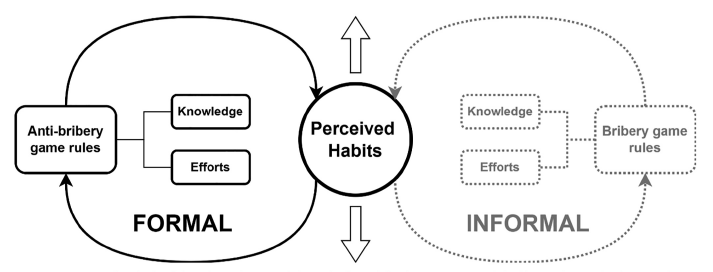
\includegraphics{theorethical-model.png}

\subsection{Papers}\label{papers}

\href{https://www.emerald.com/insight/content/doi/10.1108/ARLA-04-2022-0099/full/html}{Institutionalization
of corporate bribery: a measurement proposal with evidence from a Latin
American sample}

\href{https://www.routledge.com/Organizational-Corruption-Crime-and-Covid-19-Upholding-Integrity-and-Transparency-in-Times-of-Crisis/Stachowicz-Stanusch-Amann-Hauser-Kleinhempel-Tripathi/p/book/9781032548845}{4.
Is corporate bribery institutionalized in Latin America? Evidence from a
comparative study in seven countries}

\subsection{}\label{section}

\href{642_analisis_factorial.docx}{Ejemplo de medición}

\begin{enumerate}
\def\labelenumi{\arabic{enumi}.}
\item
  Escudriñar el documento.
\item
  Tomar nota a cerca de todas las inquietudes que este documento genera.
\item
  Intentar responderlas por cuenta propia.
\item
  Compartirlas en el documento del grupo.
\item
  Responda unas preguntas:
\end{enumerate}

\begin{itemize}
\item
  ¿Alguna de las dimensiones del índice es inconsistente?
\item
  ¿Qué dimensión es más consistente?
\item
  ¿Qué dimensión presenta una mayor redundancia?
\item
  ¿Cómo se evalúa la consistencia externa?
\end{itemize}

\bookmarksetup{startatroot}

\chapter{Tópicos}\label{tuxf3picos}

\section{Reducción de dimensiones}\label{reducciuxf3n-de-dimensiones}

Necesitamos reducir las dimensiones de un conjunto de datos por varias
razones:

\begin{itemize}
\item
  Visualización: poder observar los datos en 2 o 3 dimensiones.
\item
  Resumen: poder resumir indicadores (mediciones directas) en índices
  (mediciones indirectas).
\item
  Modelaje: poder disminuir la cantidad de variables que entran en un
  modelo.
\end{itemize}

\section{ACP}\label{acp}

El análisis de componentes principales es un método de reducción de
dimensiones basado en proyecciones de espacios vectoriales.

\subsection{Definición matemática}\label{definiciuxf3n-matemuxe1tica}

Dado un conjunto de variables \(X\) el procedimiento encuentra
coeficientes \(\alpha\) que maximizan la información explicada en su
combinación lineal \(Z\), así:

\[Z = X\alpha = \sum_{i=1}^k \alpha_i X_i\]

\subsection{Significado matemático}\label{significado-matemuxe1tico}

Esto significa una rotación en el espacio, cambiando los ejes previos
por ejes nuevos.

\section{ACP}\label{acp-1}

\subsection{Características}\label{caracteruxedsticas}

\begin{itemize}
\tightlist
\item
  Es lineal: las transformaciones que contempla son lineales.
\item
  Es interpretable: es posible establecer cuál variable es más o menos
  importante.
\item
  Los ejes son interpretables a posteriori.
\end{itemize}

\subsection{Ejemplo}\label{ejemplo-4}

\begin{itemize}
\tightlist
\item
  \href{http://setosa.io/ev/principal-component-analysis/}{setosa.io}
\end{itemize}

\section{ACP}\label{acp-2}

\subsection{Evaluación}\label{evaluaciuxf3n}

El procedimiento produce:

\begin{itemize}
\item
  Un círculo de correlaciones: Deben estar las flechas apuntando todas
  en la misma dirección.
\item
  Un gráfico de sedimentación: El primer componente debe tener un valor
  alto y los demás deben ser bajos.
\end{itemize}

\section{Alpha de Cronbach}\label{alpha-de-cronbach}

\subsection{Consistencia interna}\label{consistencia-interna-1}

En los casos donde todas las variables son mediciones indirectas
distintas de un mismo aspecto no medible, se hace referencia a la
propiedad denominada consistencia interna. La consistencia interna
consiste en la propiedad de las variables en estar altamente
correlacionadas entre sí, lo que indica que están asociadas a un trazo
latente. Dado que esta consistencia interna se encuentra reflejada en a
estructura de correlación de las variables es posible medirla y
analizarla.

\section{Alpha de Cronbach}\label{alpha-de-cronbach-1}

El Alfa de Cronbach (\textbf{Cronbach1951?}) es una de las medidas más
usadas para analizar la consistencia entre variables.

Dados \(K\) variables \(Y_1, Y_2, ..., Y_K\) y su suma
\(X = Y_1 + Y_2 + ... + Y_K\), el Alfa de Chronbach está dado por la
expresión

\[\alpha = \frac{K}{K-1} \left(1-\frac{\sum_{i = 1}^K \sigma^2_{Y_i}}{\sigma^2_X}\right)\]

\section{Alfa de Cronbach}\label{alfa-de-cronbach}

\begin{quote}
El valor mínimo aceptable para el coeficiente alfa de Cronbach es 0,70;
por debajo de ese valor la consistencia interna de la escala utilizada
es baja. Por su parte, el valor máximo esperado es 0,90; por encima de
este valor se considera que hay redundancia o duplicación.
\end{quote}

\href{http://scielo.org.co/pdf/rcp/v34n4/v34n4a09.pdf}{Aproximación al
uso del coeficiente alfa de Cronbach}

\bookmarksetup{startatroot}

\chapter{Referencias}\label{referencias}

Cohen, R. J., Swerdlik, M. E., \& Phillips, S. M. (1996). Psychological
testing and assessment: An introduction to tests and measurement.
Mayfield Publishing Co.




\end{document}
